% !Mode:: "Tex:UTF-8"
\chapter{不依赖位置信息的拓扑骨干提取}
\label{chap:3}
不依赖位置信息的拓扑骨干提取是无线传感器网络拓扑压缩的重要问题。仅利用连通性信息的拓扑骨干提取是一项非常具有挑战性的研究内容。目前已有的一些方法在一定的网络假设条件下被证明是非常有效的,但往往具有各自的局限性。有些方法基于连续域的思想,在扩展至离散网络中具体的算法时往往产生一定的失真和网络开销;有些方法无法得到确定性的结果,或严格依赖于均匀、稠密部署的网络假设。本章提出了一种仅利用局部连通性信息,且能够得到确定性拓扑骨干的鲁棒的拓扑骨干提取算法。算法分别利用了不依赖位置信息的骨干节点提取方法、高效的图理论变换工具HPT(homotype preservation transformation),以及骨干叶节点判定方法等,能够有效地适用于具有各种不同形状和参数设置的网络。本章从理论上证明了算法的有效性,并通过大量的仿真实验验证了算法的性能。
\section{引言}
在无线传感器网络中,节点的分布以及全局的拓扑结构是网络中大部分功能和协议的基础。由于受到节点部署的随机性、网络区域的几何形状、区域内的障碍物等因素的影响,网络的拓扑结构通常具有复杂的特征。这些拓扑特征对于网络中很多协议的设计和运行具有重要的影响。拓扑骨干是对网络全局拓扑特征的一种重要描述,因此成为无线传感器网络中一个重要的研究问题。拓扑骨干可以被有效地利用来改善一系列位于其上层的网络协议和算法的性能,如路由协议\upcite{skeleton_mobihoc05,skeleton_wn}、定位算法\upcite{localization_infocom08,skeleton_localization}、网络分区(segmentation)\upcite{segmentation_infocom07,segmentation_concel,segmentation_infocom12}、导航(navigation)\upcite{navigation_infocom06}等。

骨干提取问题源自计算机视觉\upcite{skeleton_vision}和计算机图形学\upcite{skeleton_graphics},并在多年来得到了广泛的研究。但是与传统的计算机视觉和图形学不同,无线传感器网络的拓扑骨干无法利用连续域中的属性来描述。在离散的网络中,节点之间的距离通常是通过跳数距离来表示,而无法利用连续域中的精确的欧式距离来度量。离散网络中的拓扑骨干的提取一般需要两个过程:首先从网络中提取出一定数量的骨干节点,然后将这些骨干节点连接起来构成骨干网络。然而,在仅利用连通性信息的情况下,骨干节点的判定往往容易受到一些噪声信息的干扰,如不完整或者不准确的边界信息、跳数距离和欧式距离之间的偏差等。另外,即使能够获得一定数量的准确的骨干节点,如何将这些骨干节点连接起来形成连通的、符合网络实际几何形状的拓扑骨干,仍然是一个非常有挑战性的问题。

目前已有的不依赖位置信息的拓扑骨干提取算法在不依赖节点位置的情况下,提供了一定程度的有效机制来抽取出网络的拓扑骨干。但这些方法往往严格地依赖于一定的网络假设条件,或者是基于启发式的方法,而无法从理论上证明提取出的拓扑骨干的连通性,又或者可能出现不确定的结果,无法保证结果符合网络实际的几何形状。例如,MAP\upcite{skeleton_mobihoc05,skeleton_wn}、CASE\upcite{skeleton_infocom09}、DIST\upcite{skeleton_icdcs12}等方法,以完整或部分的边界节点信息作为输入,设计了不同的骨干节点判定方法,并利用一系列启发式的操作将这些骨干节点连接起来形成骨干网络。但这些方法均严格地依赖于已知的边界节点信息。当存在边界噪声时(即不准确的边界节点信息),方法的性能较差,甚至无法得到有效的连通拓扑骨干。Liu等人\upcite{skeleton_icdcs122}提出了一种不依赖边界节点信息的骨干提取算法。该算法利用连续域中的观察结果,即点越靠近图形的中心位置,以该点为圆心嵌入的圆盘的面积越大。将这一观察结果扩展至离散网络中,就可以得到骨干节点的判定原则,即骨干节点拥有更多的邻居节点。但由于实际的离散网络与连续域存在较大差别,该算法的性能受到节点分布情况的影响较大。当节点部署的随机性较强,或节点分布比较稀疏时,该算法输出的拓扑骨干的质量将严重下降,甚至无法得到正确的拓扑骨干。综上所述,不依赖位置信息的拓扑骨干提取问题目前仍没能得到很好的解决。

本章致力于设计仅利用局部连通性信息的鲁棒的拓扑骨干提取算法。首先,我们利用局部的MDS(multidimensional scaling)方法设计了高效的边界节点识别算法,并进一步设计了不依赖位置信息的骨干节点识别算法。为了提高对边界噪声的鲁棒性,我们提出将骨干节点扩展为骨干带网络,并设计了高效的图理论变换工具HPT,用于从骨干带网络中抽取出初始骨干网络。最后,算法利用局部的剪枝操作对初始骨干网络进行修剪,得到了高质量的拓扑骨干。本章从理论上证明了算法提取出拓扑骨干的连通性,并通过大量的仿真实验验证了算法的性能和良好的鲁棒性。

本章余下的部分组织如下:3.2节介绍本章采用的基本网络设置和假设;3.3节详细介绍了不依赖位置信息的拓扑骨干提取算法的设计;3.4节通过大量的仿真实验检验方算法的有效性和性能;最后3.5节对本章进行总结。
\section{问题描述}
本节主要给出本章中所采用的基本网络配置和假设。

首先,本章假设节点部署在平面区域,每个节点仅能与位置临近的其它节点通讯,节点的坐标是未知的,节点间不能确定相互的距离和方位。本章将网络通讯的连通关系图建模为一个简单无向图$G(V,E)$,其中点集$V$表示传感器节点,边集$E$表示节点之间直接的通讯链路。

其次,本章假设网络中的每个节点都能够收集本节点的$k$跳邻居信息,获得局部的$k$跳邻居子图。邻居信息的获取可以通过一个范围为$k$的局部洪泛消息来实现。一般情况下,参数$k$只需设置为一个较小的常数,例如$k$取值为3 时就可以满足本章所涉及到绝大部分网络实例的需求。这一假设是比较松弛和可行的,实际上已经是无线传感器网络基于连通性信息的相关研究中最放松的网络假设。在本章中,$N_G^k(v)$表示到顶点$v$的最短距离不大于$k$的邻居集合;$G(X)$表示由顶点集$X$生成的网络子图,即由$X$中顶点和它们之间的边组成的子图;顶点$v$的$k$跳邻居子图就可以表示为$G_k(v)=G(N_G^k(v))$。$G$中边$e=(u,v)$的$k$跳邻居子图$G_k(e)$定义为$G_k(e)=G((N_G^k(u)\cap{N_G^k(v)})\cup\{u,v\})-e$。默认情况下,$N_G(v)$(或$N_G(e)$)和$G(v)$(或$G(e)$)分别表示点$v$(或边$e$)的1跳邻居集合和1跳邻居子图。
\section{拓扑骨干提取算法}
本节介绍不依赖位置信息的拓扑骨干提取方法的具体设计。首先概述方法的基本思想和大致过程,然后对方法中几个重要的步骤分别进行详细的介绍,最后给出具体的算法,并对算法中一些关键的参数及其对算法性能的影响进行讨论。
\subsection{方法概述}
骨干最早是来自于连续域中的概念,是对对象几何形状的一种重要描述。随着拓扑骨干问题被引入到无线传感器网络中,大部分的研究工作仍然是基于连续域中的某些观察结果,并将其扩展至离散网络中的拓扑骨干提取算法。但是,由于离散网络与连续域之间采用了不同的距离度量方式,使得在具体的算法设计过程中引入了较大的失真。而且,算法实际的执行效果受到网络参数的显著影响。因此,在仅利用连通性信息的情况下,设计鲁棒的拓扑骨干提取算法是非常具有挑战性的。目前已有的一些方法往往基于某种特定的网络假设,或对网络部署的密度和均匀性有较高的要求。本章致力于提出一种鲁棒的拓扑骨干提取方法,在仅利用局部连通性信息的情况下,从具有各种复杂形状和不同参数设置的网络中提取出确定性、高质量的拓扑骨干。

下面介绍本章提出的拓扑骨干提取算法的主要思想。首先,利用边界识别算法提取出网络边界节点,并利用边界节点信息提取出一定数量的骨干节点。然后,对骨干节点进行扩展得到一个具有良好连通性的骨干带网络,并在此基础上设计了一种高效的图理论工具HPT,用来从骨干带网络中抽取出具有良好形状和连通性的初始骨干。最后,通过剪枝操作对初始骨干进行修正,得到最终的拓扑骨干。为了叙述的方便,我们将整个算法分为四个主要的组件,分别是边界识别、骨干节点提取、原始骨干提取、剪枝修正,并通过图\ref{fig:301}所示的例子对算法的执行过程进行介绍。对于图\ref{fig:301a}所示的网络连通图,算法最终将从中提取出图\ref{fig:301h}中粗线所示的拓扑骨干。
\begin{figure}[t]
  \centering
  \subfloat[网络连通图]{
    \label{fig:301a}
    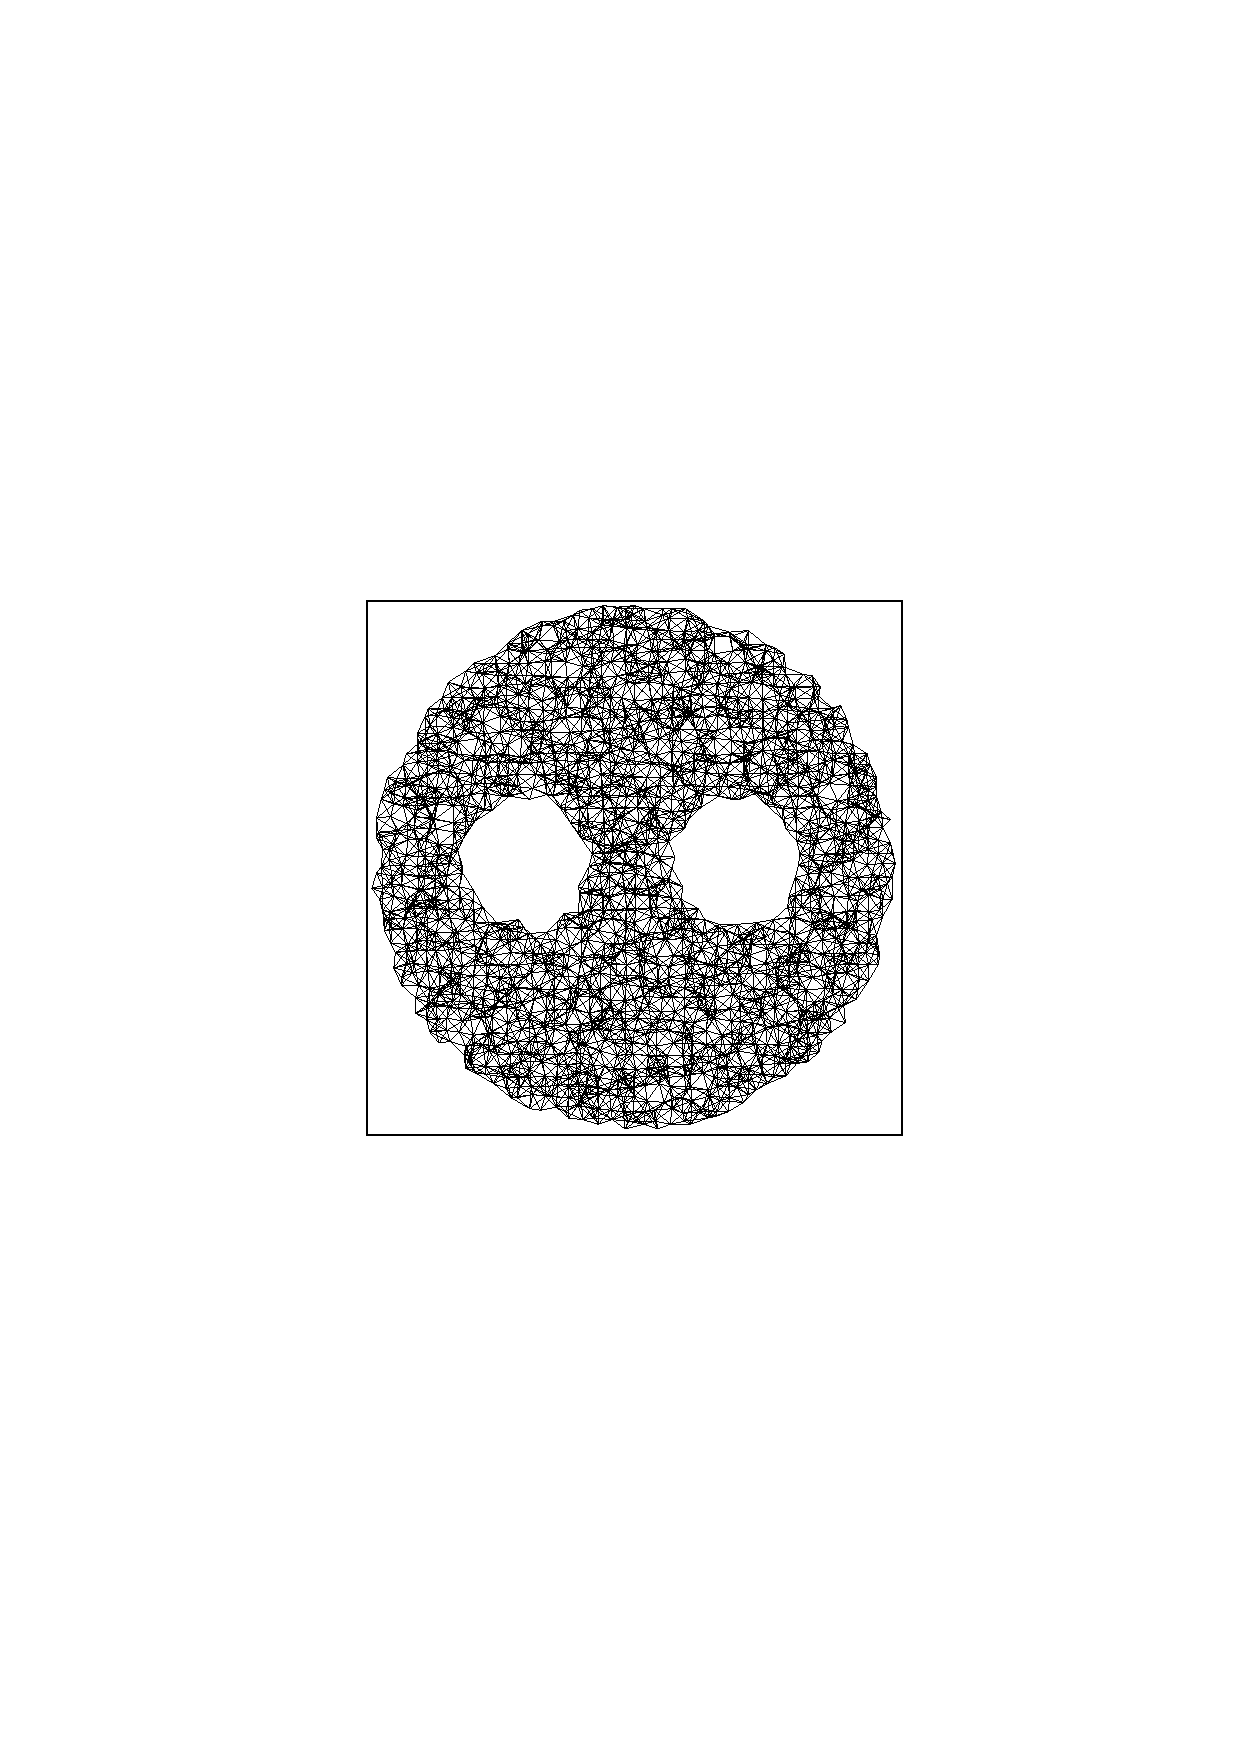
\includegraphics[width=.3\textwidth]{fig301-a}}\hspace{0.25em}%
  \subfloat[边界节点识别]{
    \label{fig:301b}
    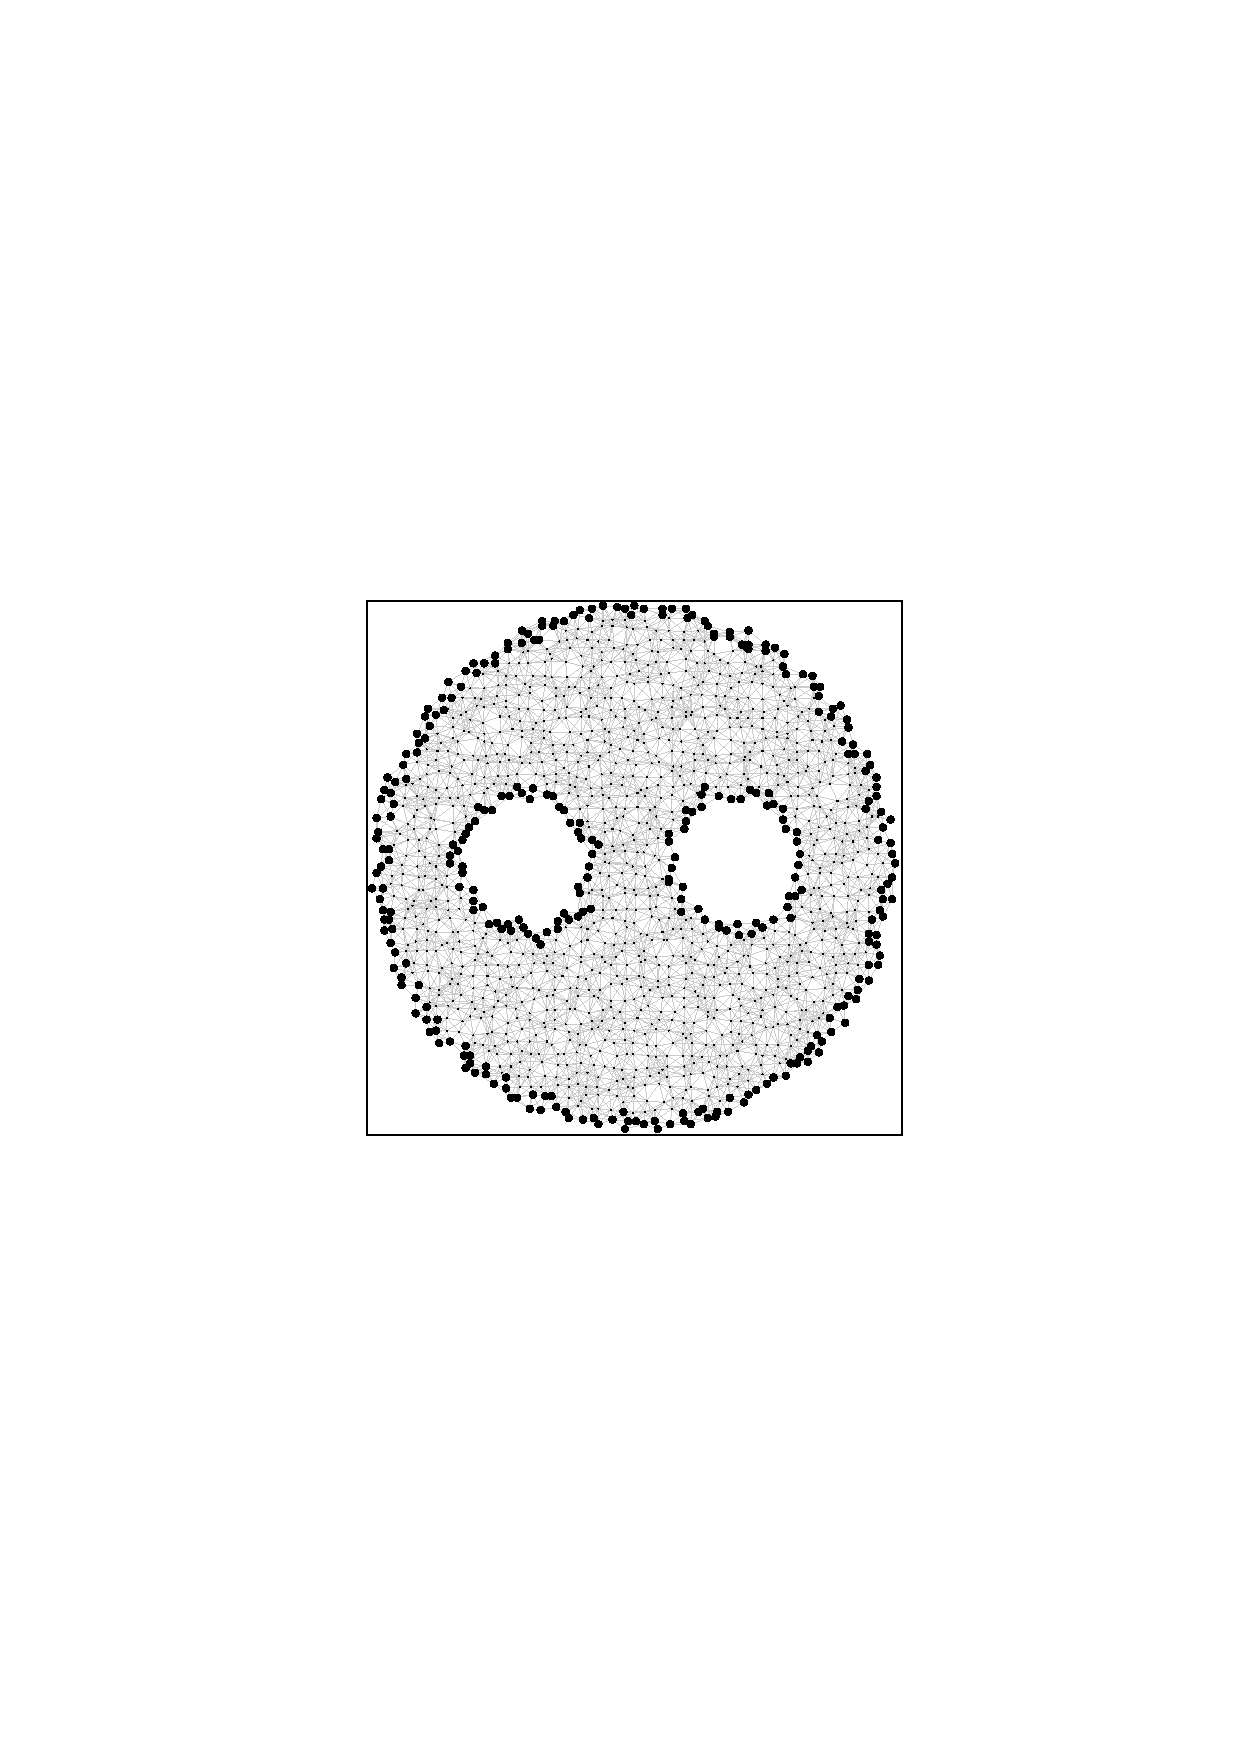
\includegraphics[width=.3\textwidth]{fig301-b}}\hspace{0.25em}%
  \subfloat[边界连通分支]{
    \label{fig:301c}
    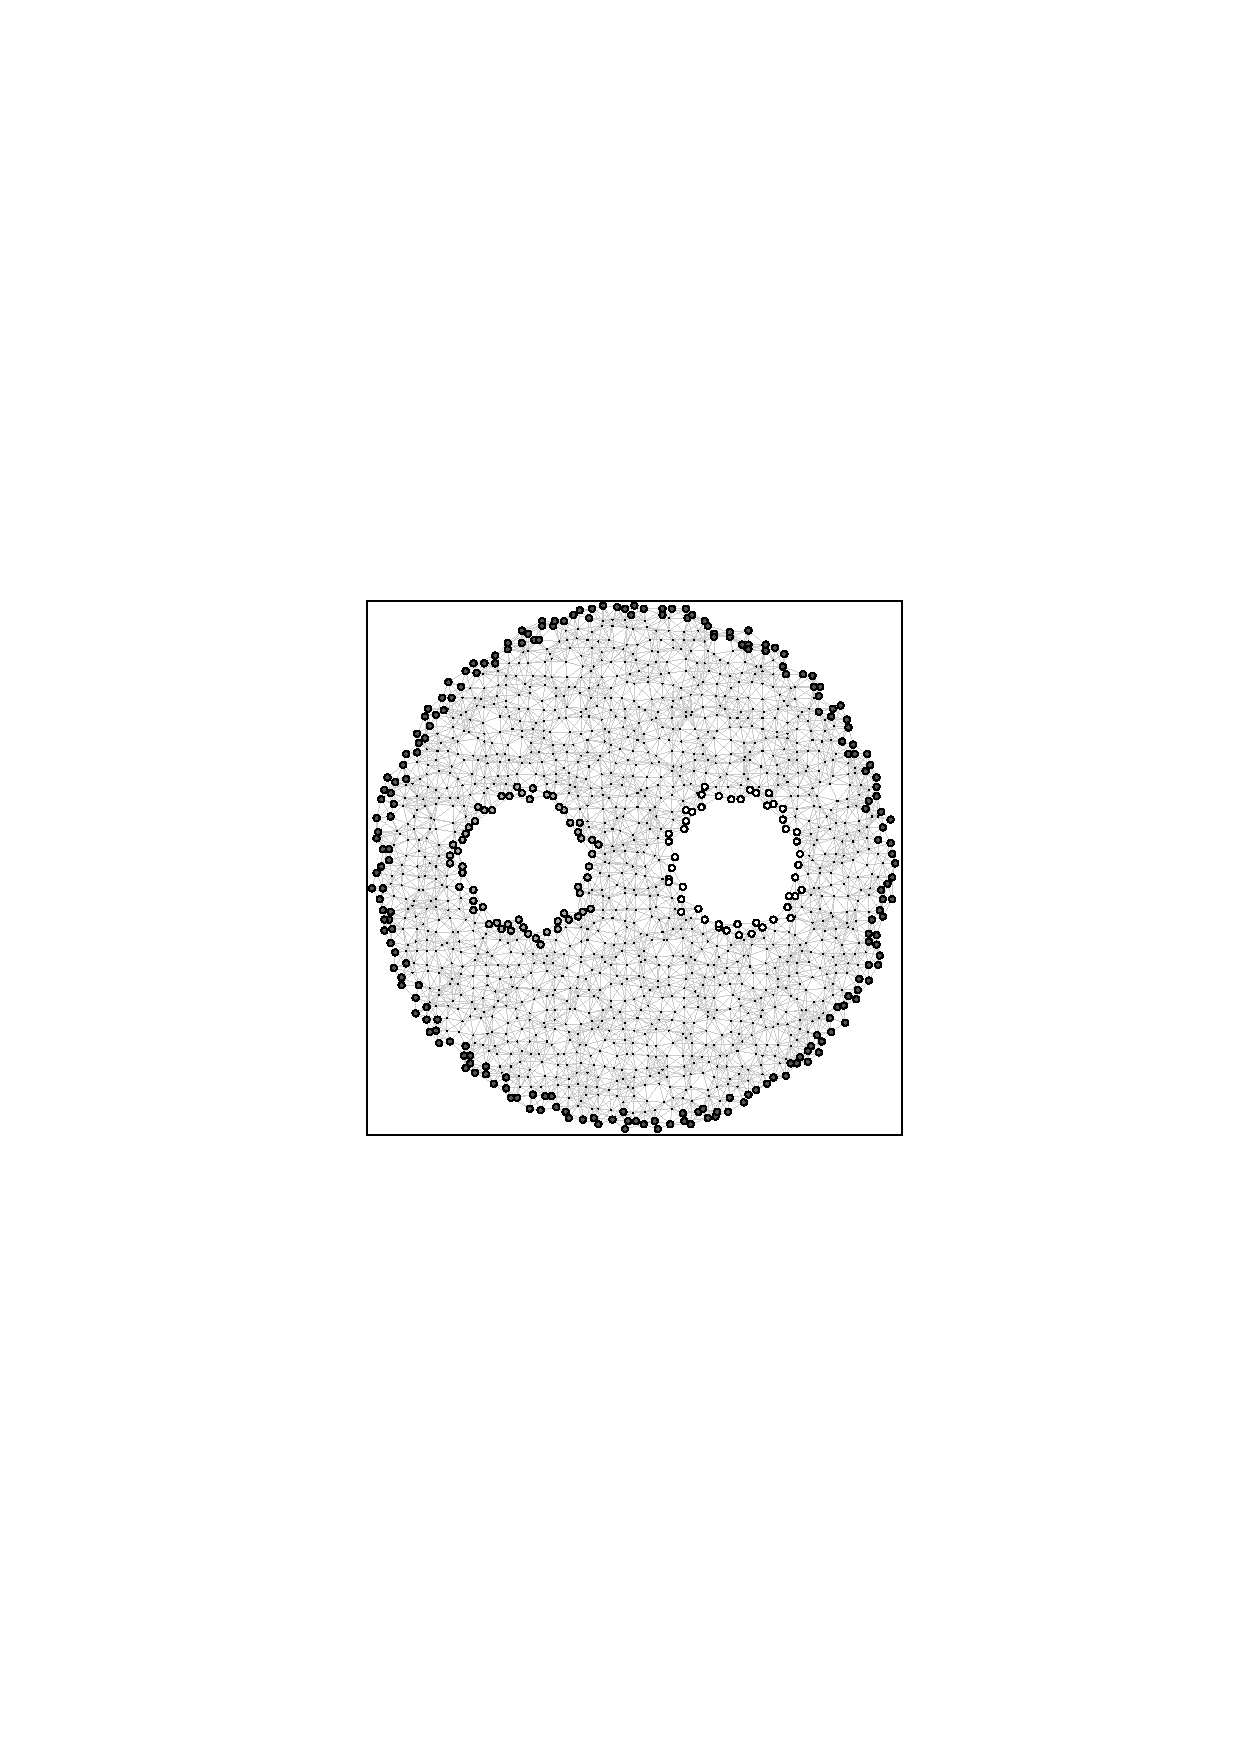
\includegraphics[width=.3\textwidth]{fig301-c}}\hspace{0.25em}%
  \subfloat[骨干节点识别]{
    \label{fig:301d}
    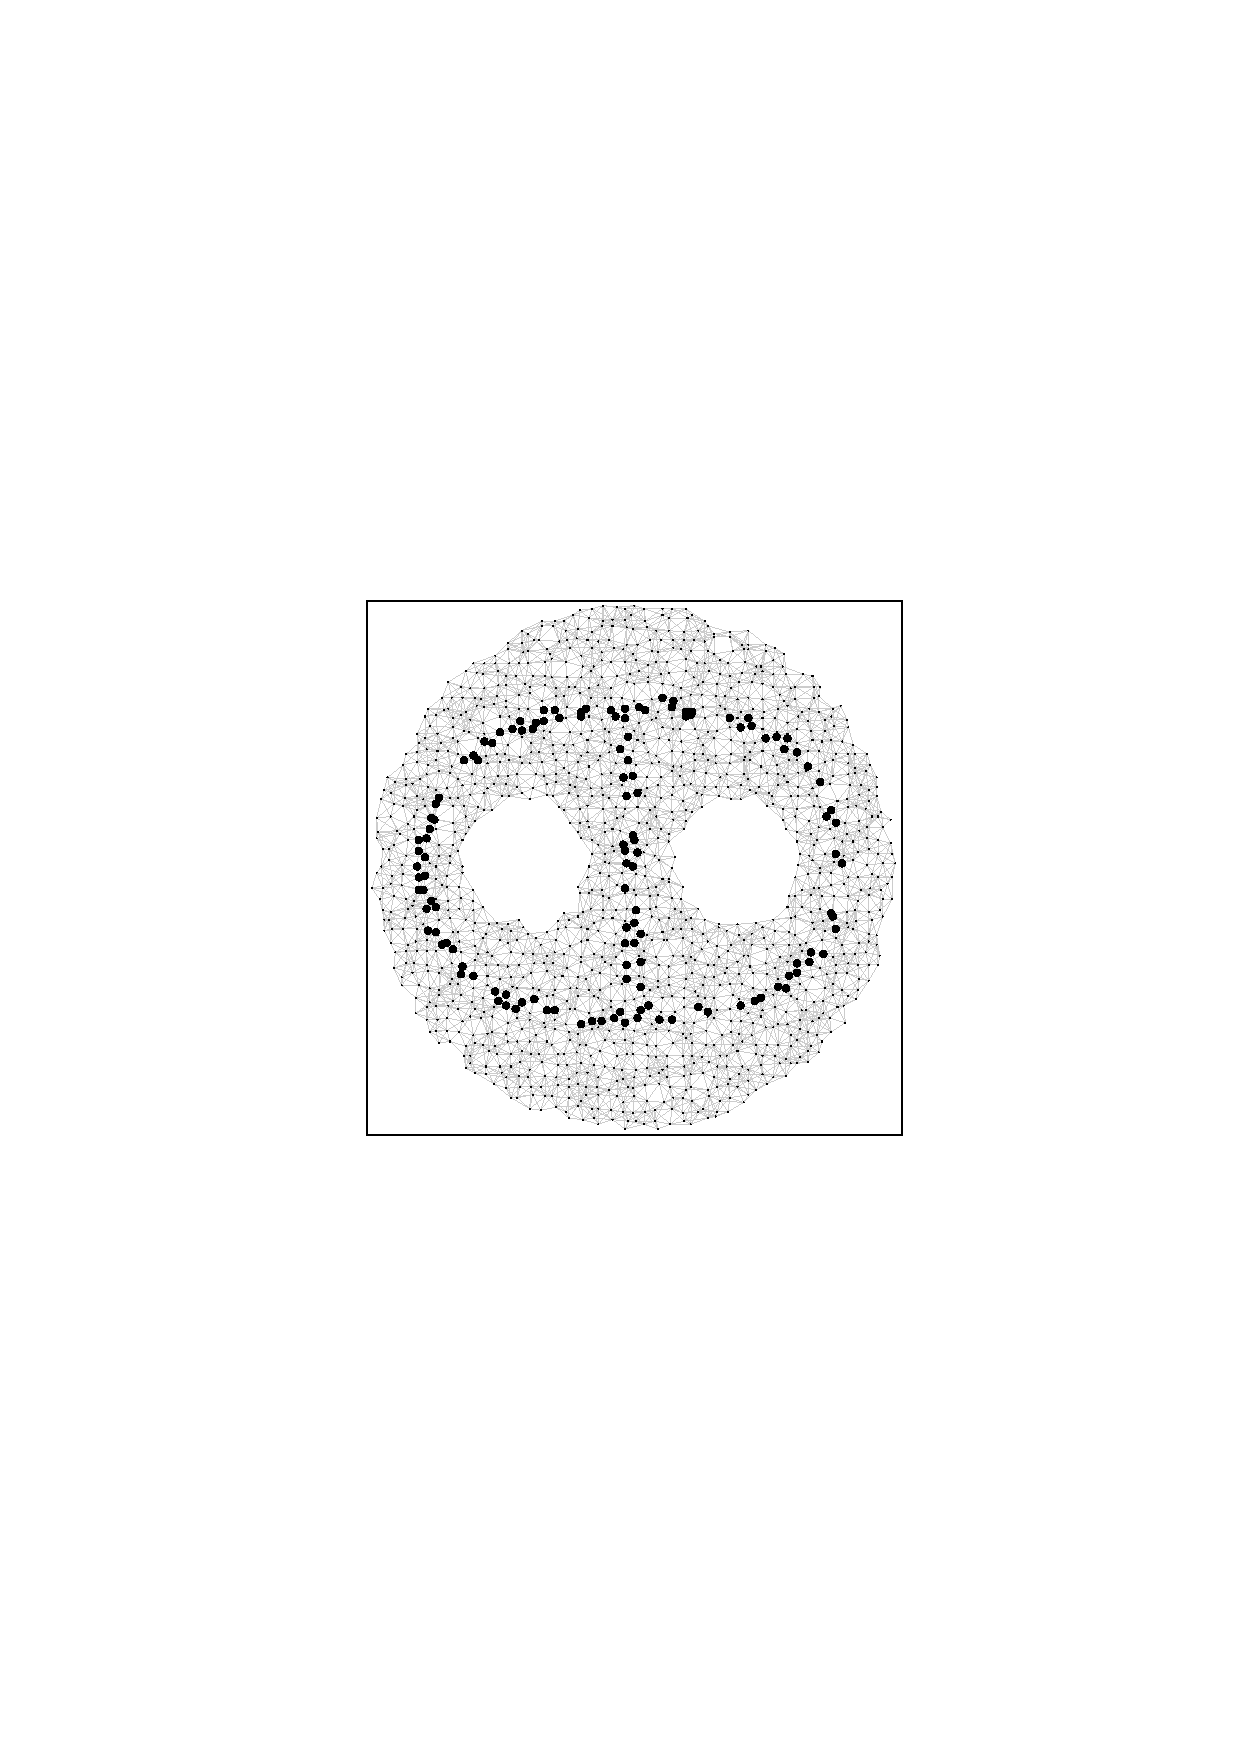
\includegraphics[width=.3\textwidth]{fig301-d}}\hspace{0.25em}%
  \subfloat[骨干节点扩展]{
    \label{fig:301e}
    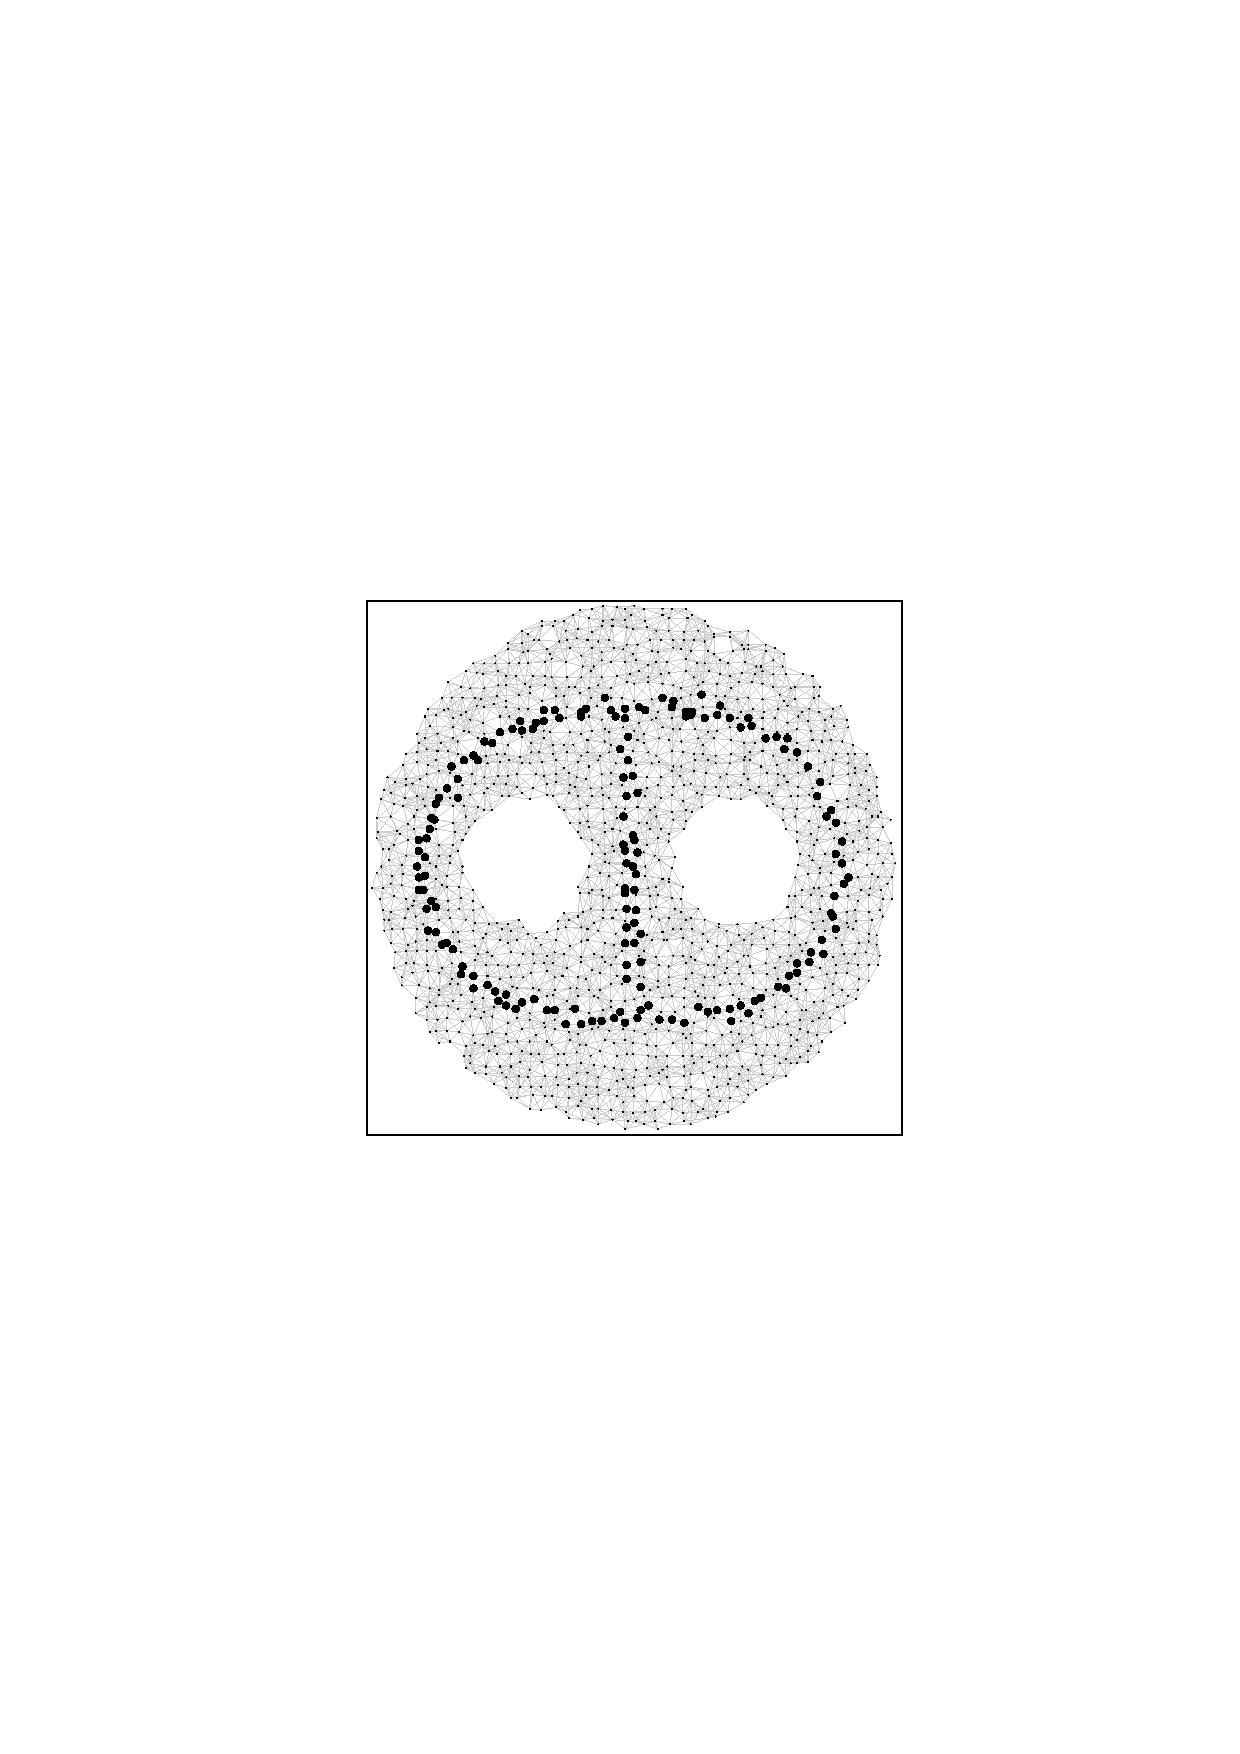
\includegraphics[width=.3\textwidth]{fig301-e}}\hspace{0.25em}%
  \subfloat[构建骨干带网络]{
    \label{fig:301f}
    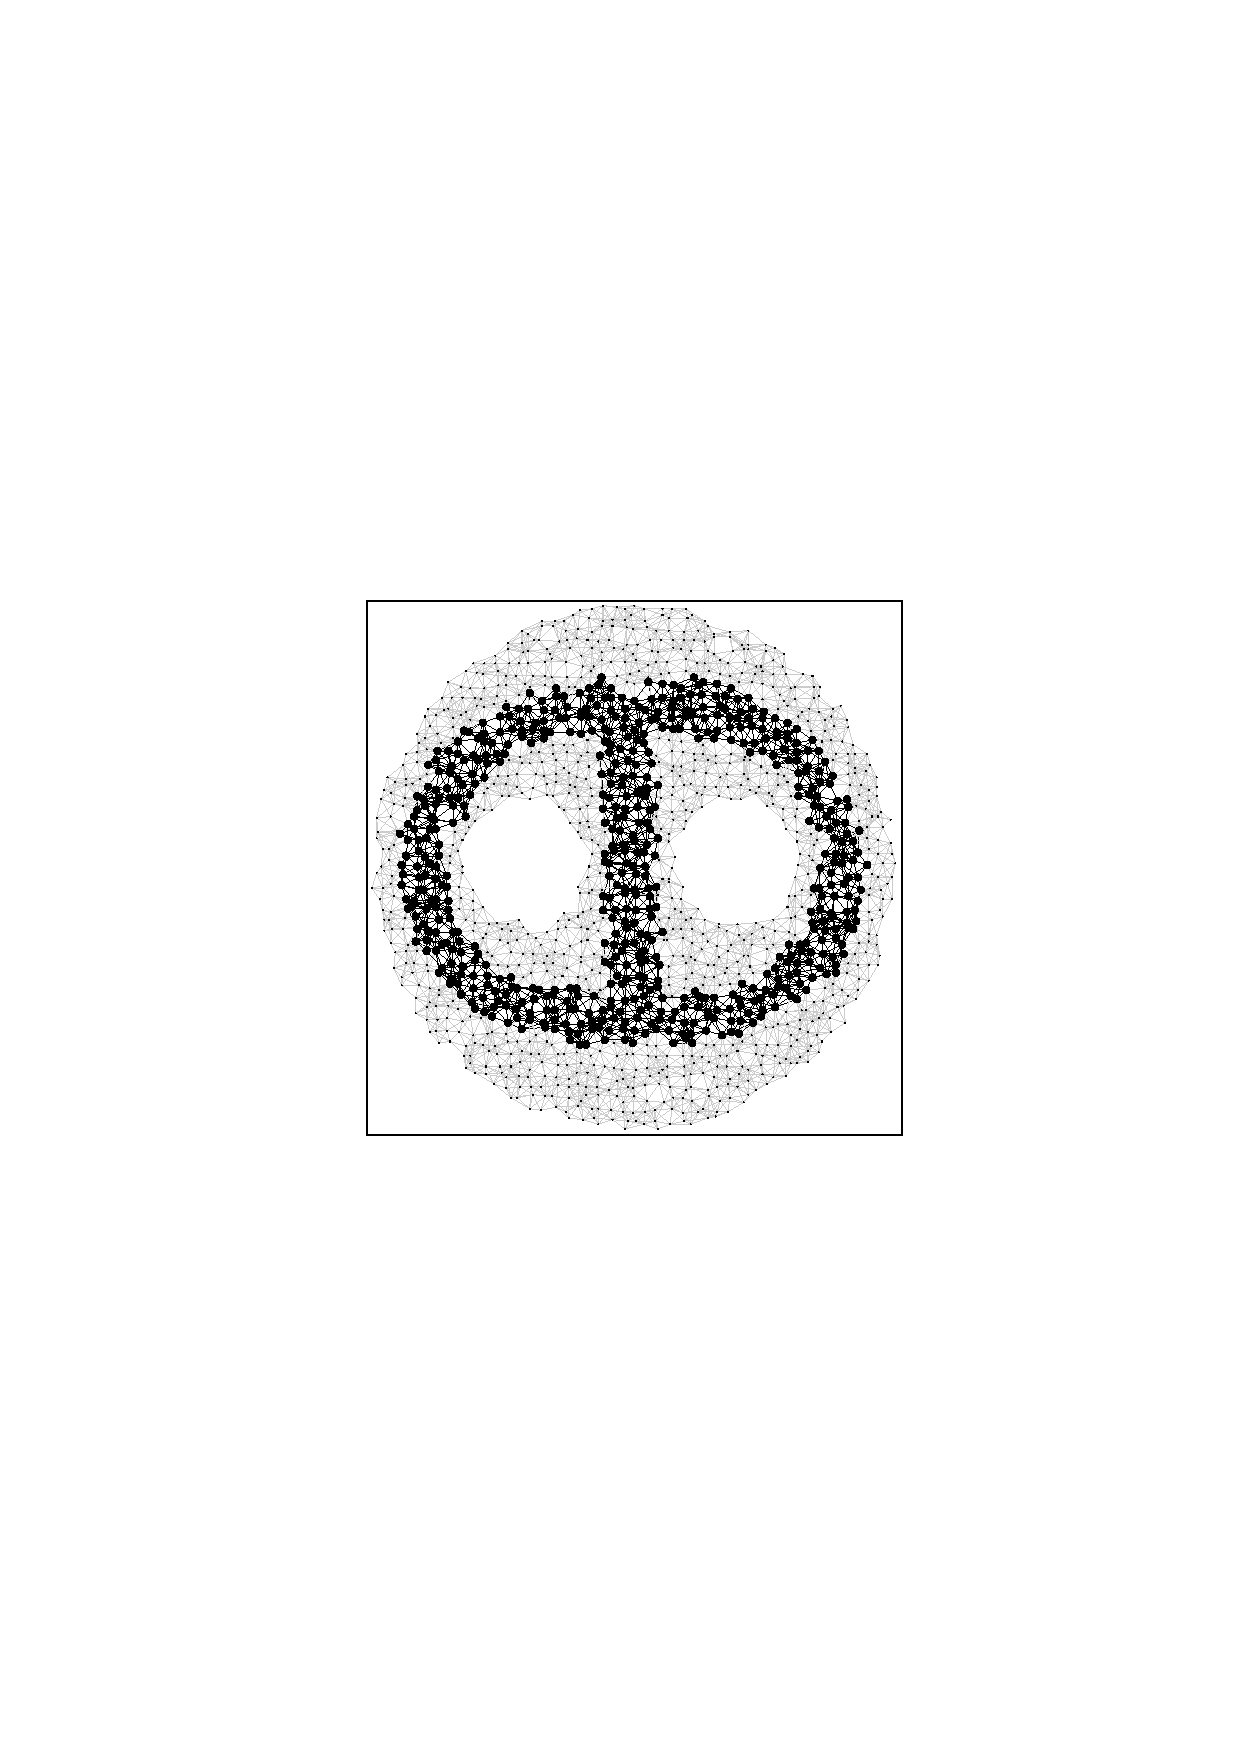
\includegraphics[width=.3\textwidth]{fig301-f}}\hspace{0.25em}%
  \subfloat[初始骨干]{
    \label{fig:301g}
    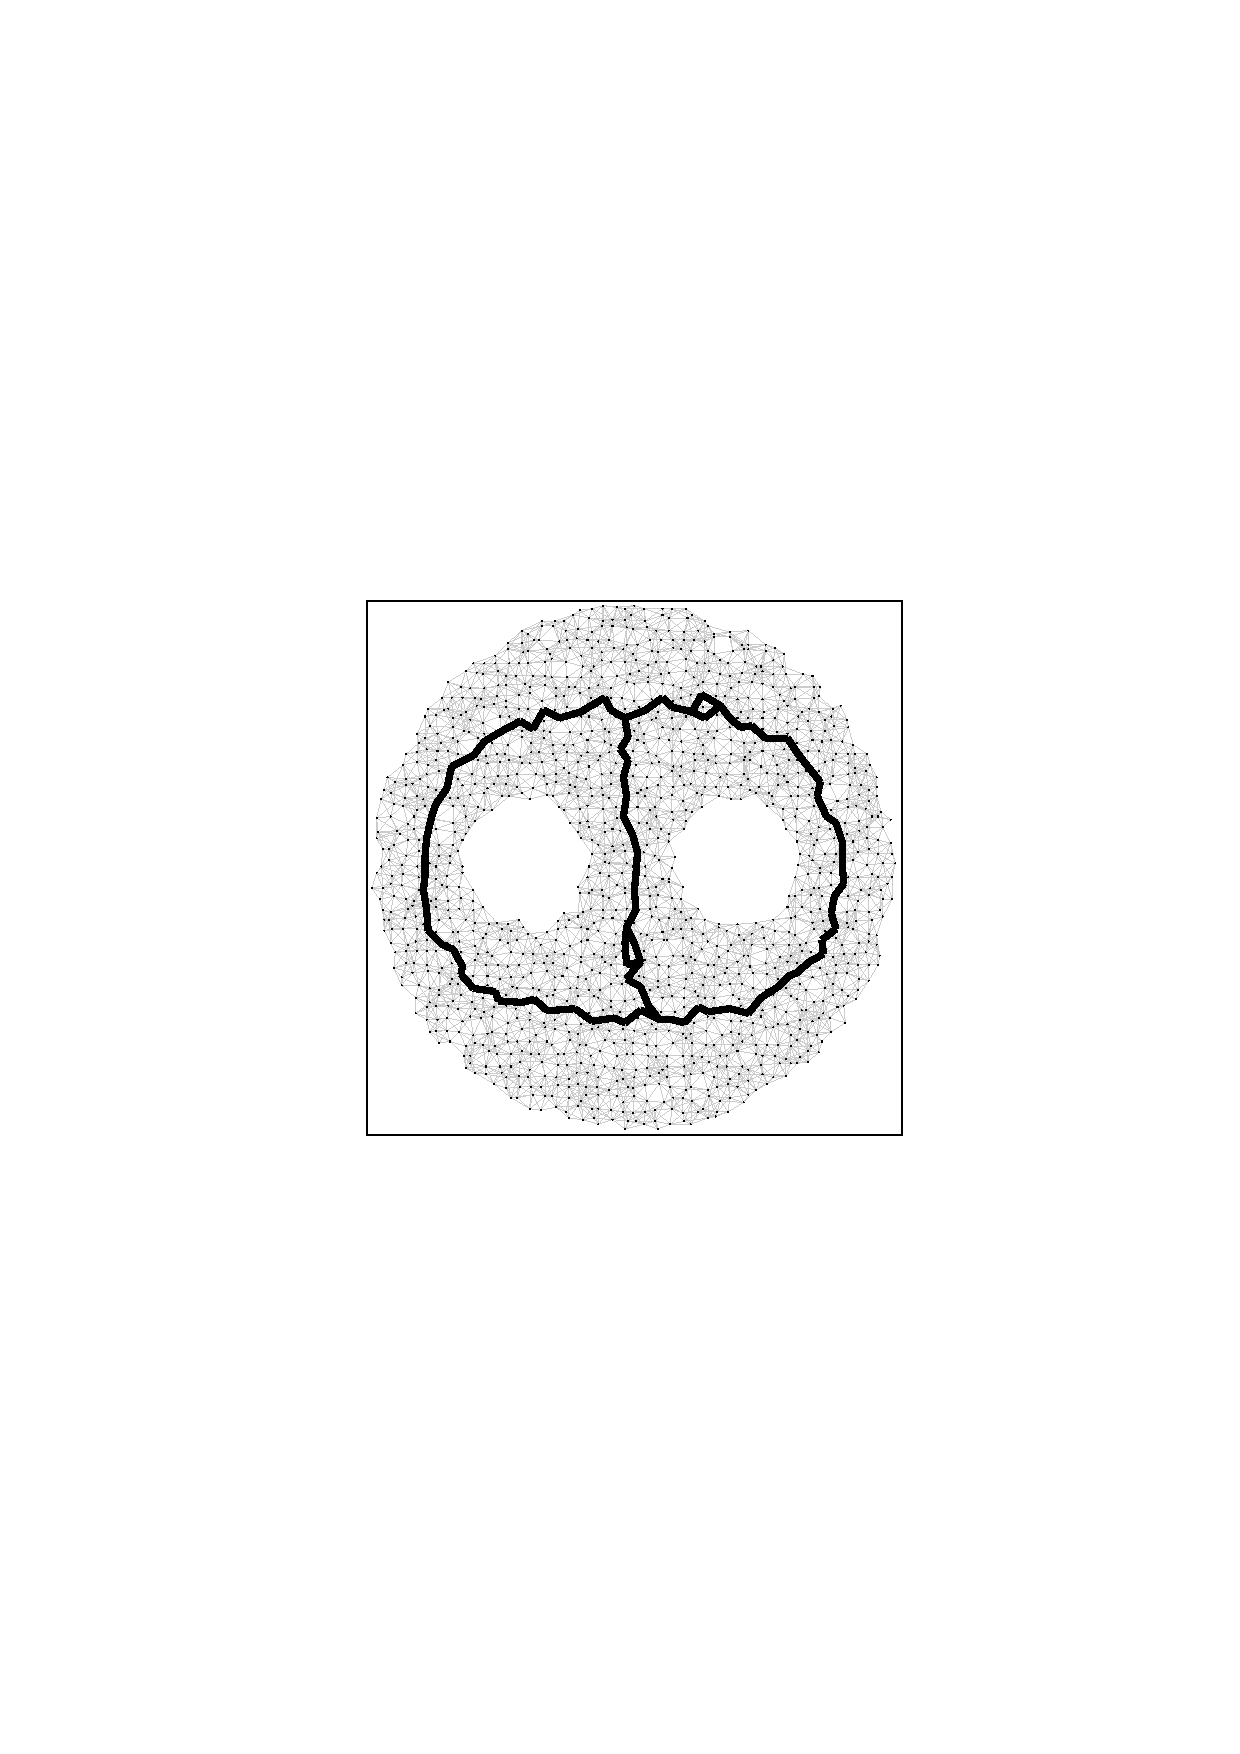
\includegraphics[width=.45\textwidth]{fig301-g}}\hspace{0.25em}%
  \subfloat[最终的拓扑骨干]{
    \label{fig:301h}
    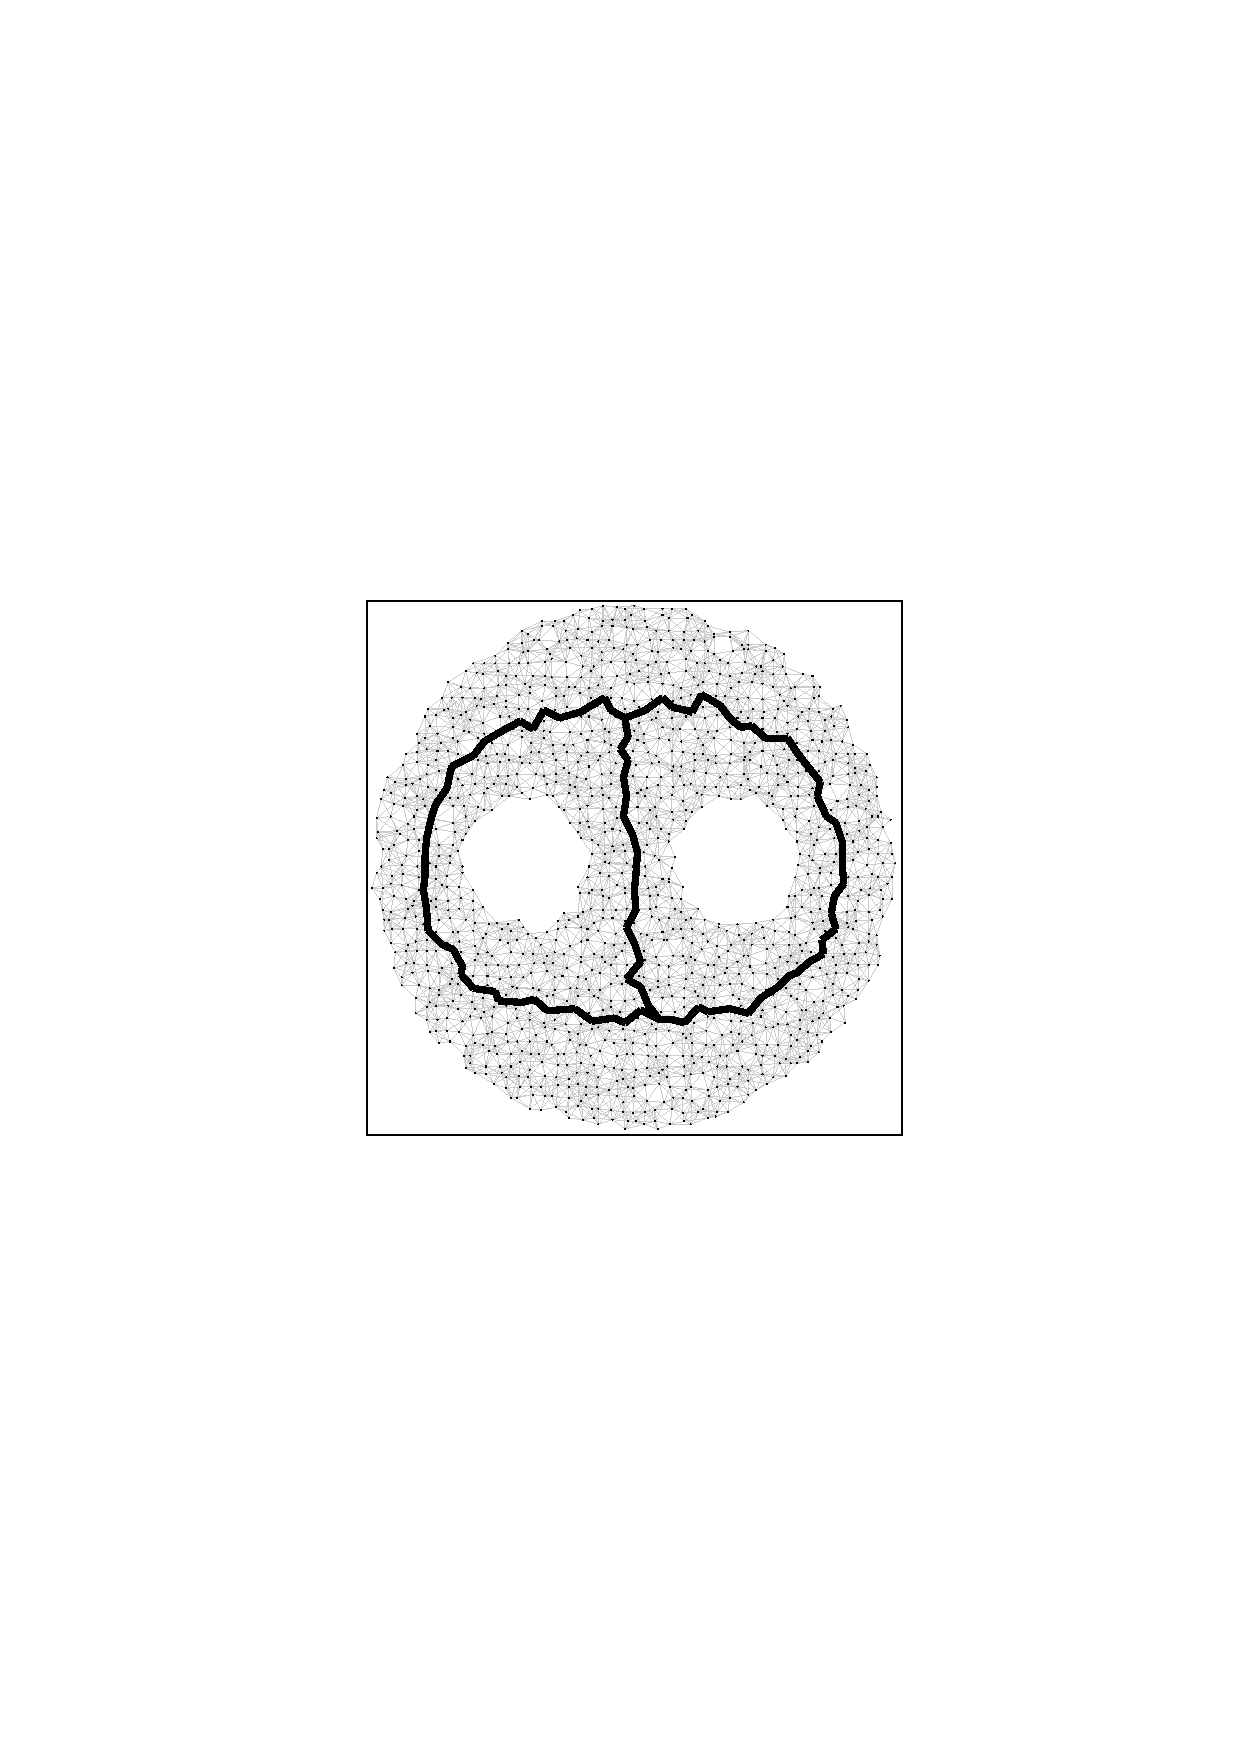
\includegraphics[width=.45\textwidth]{fig301-h}}
  \caption{拓扑骨干提取算法的执行过程}
  \label{fig:301}
\end{figure}

在边界识别组件中,我们利用了一种仅依赖局部连通性信息的基于MDS的边界识别算法,提取出网络的边界节点,如图\ref{fig:301b}所示。MDS算法将节点的局部邻居子图进行维度规约,嵌入在二维平面中,并根据嵌入的结果判断本节点是否位于网络边界上。然后对识别出的边界节点之间的连接关系进行分析,找出由边界节点组成的所有的连通分支,如图\ref{fig:301c}所示,其中不同灰度的圆圈表示不同的边界分支上的点。在骨干节点提取组件中,我们利用边界节点连通分支信息来判定骨干节点。骨干节点判定的基本思想与文献\upcite{skeleton_infocom09}类似,即对于骨干上的每个节点,至少存在两个位于不同边界分支上的边界节点到该点的最小距离相同。但是,仅利用该原则提取出的骨干节点往往比较稀疏,骨干节点之间的连通性较差,因此可能导致在此基础上提取出的拓扑骨干与网络的实际几何形状出现偏差。为了解决这一问题,我们引入了另外一种骨干节点判定准则,即骨干节点到边界的距离局部最大化原则。该判定准则的基本思想与文献\upcite{skeleton_icdcs122}类似,即某些骨干节点位于网络的中央位置,因此其到网络边界的距离是局部最大的。综合利用以上两条准则,我们就可以得到一定数量的骨干节点,如图\ref{fig:301d}所示。接下来,我们将骨干节点连接起来,形成唯一的连通分支,如图\ref{fig:301e}所示。这一操作的目的是为了进一步地改善骨干节点之间的连通性。在原始骨干提取组件中,我们首先将骨干节点进一步扩展至其一跳邻居,得到一个具有良好连通性的骨干带网络,如图\ref{fig:301f}所示。然后设计了一种分布式的图理论工具,即HPT变换工具。HTP变换的基本思想是在不引入长度大于一定门限值的环的基础上,执行点删除和边删除操作,将骨干带网络按照从外而内的顺序层层剥离,最终从中抽取出一个原始的骨干网络,如图\ref{fig:301g}所示。最后,我们利用剪枝修正组件对初始骨干中可能包含的局部的小环结构进行处理。剪枝修正组件首先以分布式的方式从初始骨干中找出长度小于预设的门限值的局部环结构,将这些环打断并进一步地修剪掉较短的分支。剪枝修正过程完成后,算法将得到最终的拓扑骨干,如图\ref{fig:301h}所示。

接下来对拓扑骨干提取算法的各个组件分别进行具体的介绍,并进行必要的理论分析和证明。
\subsection{边界识别}
本组件利用基于MDS的边界识别算法提取出网络中的边界节点。MDS技术最早源自行为科学和社会科学中对对象结构的研究,是一种对数据进行不相似度分析和可视化的技术。MDS算法以目标之间的不相似度矩阵为输入,将其嵌入至低维空间并输出规约结果。MDS的目标是创建目标在低维空间的一种实现,并使得目标之间的距离(在某种度量方式下)尽量接近原始的不相似度。目前,MDS技术已经在无线传感器网络的定位技术\upcite{mds_localization1,mds_localization2}以及边界识别技术\upcite{mds_boundary}中得到了一定的应用。不依赖位置信息的边界检测技术的主要难点就在于位置信息的缺失使得边界节点的判定缺乏依据。而MDS技术在仅有局部连通性信息的情况下,以节点间的跳数距离作为近似,对节点的局部连通图进行维度规约并嵌入在平面中。在嵌入得到的虚拟连通图中,每个节点被赋予虚拟坐标值。然后,我们就可以利用这些虚拟坐标信息来判定节点是否为边界节点。
\begin{figure}[t]
  \centering
  \subfloat[网络连通图]{
    \label{fig:302a}
    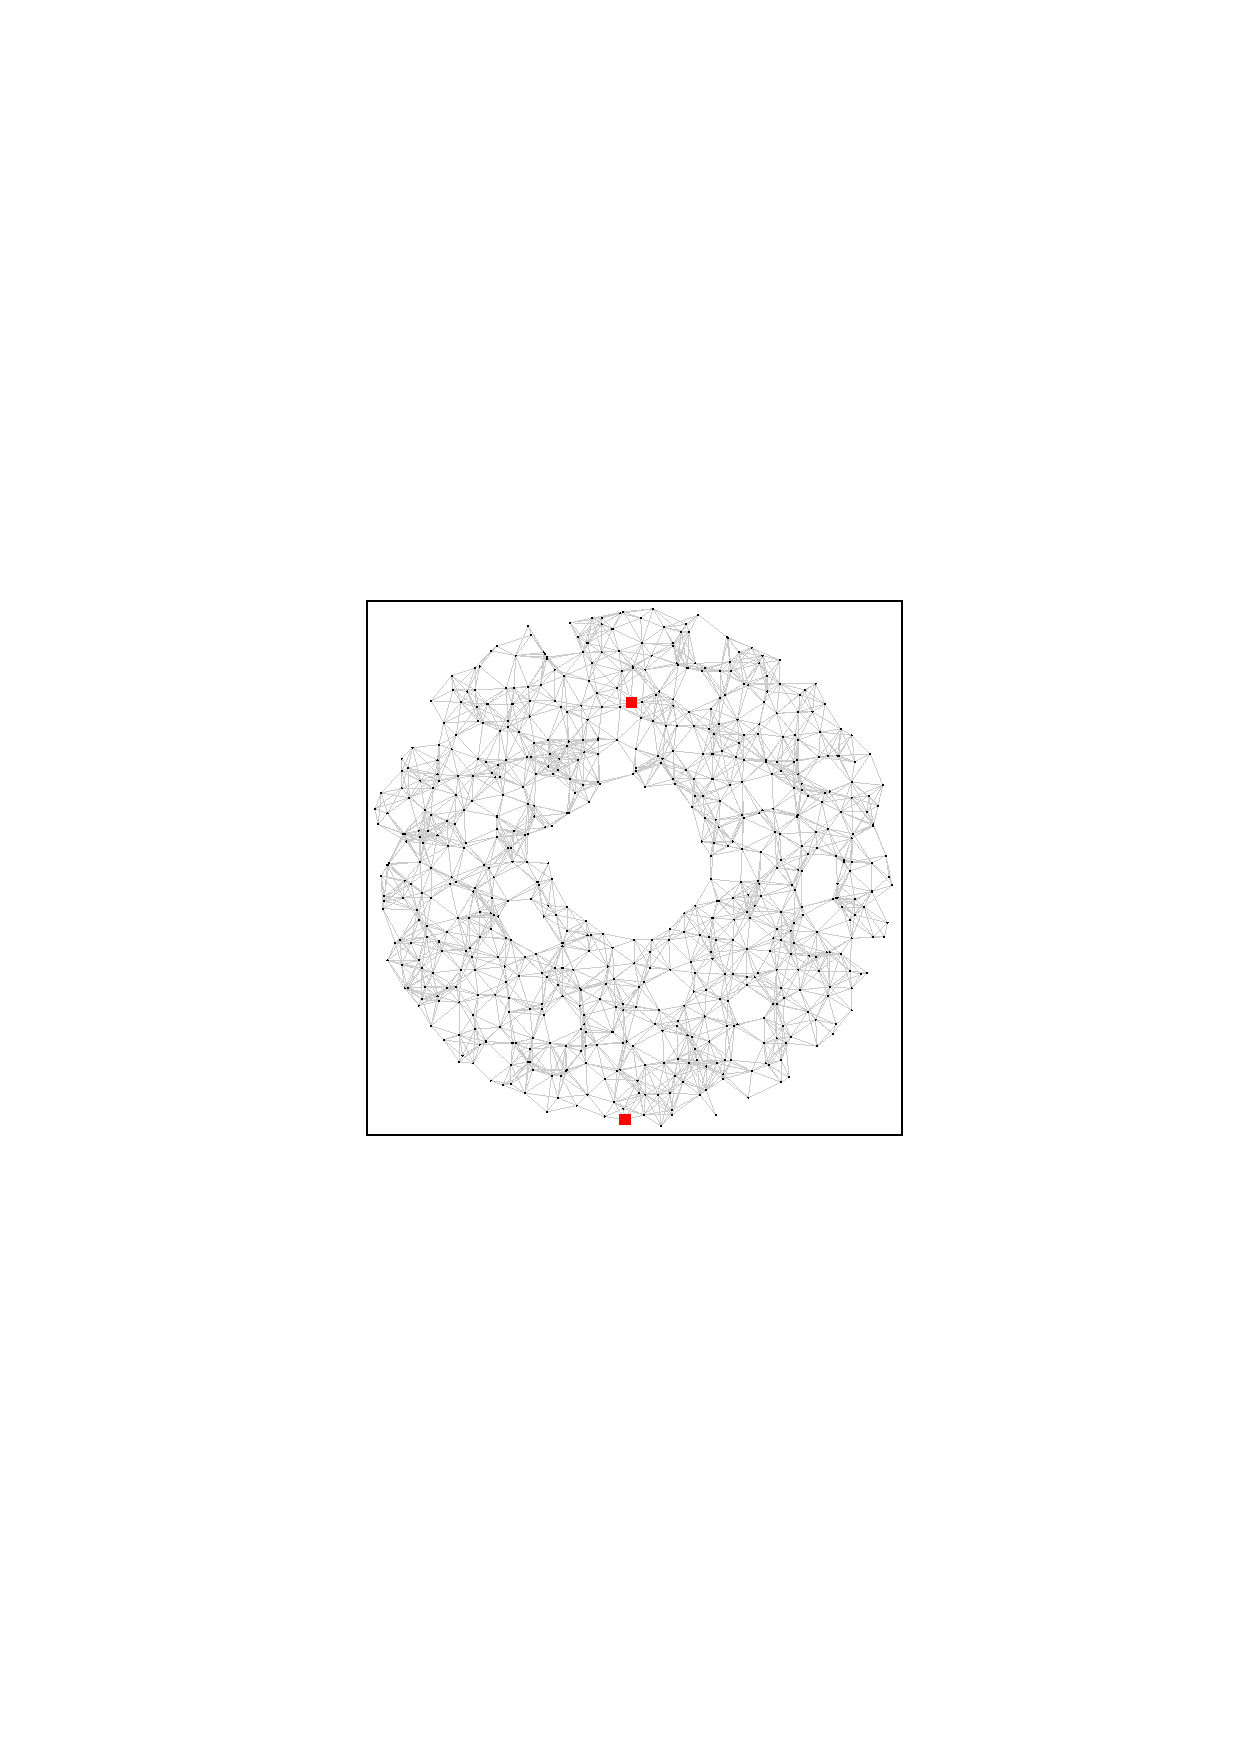
\includegraphics[width=.3\textwidth]{fig302-a}}\hspace{0.25em}%
  \subfloat[内部节点的局部连通图]{
    \label{fig:302b}
    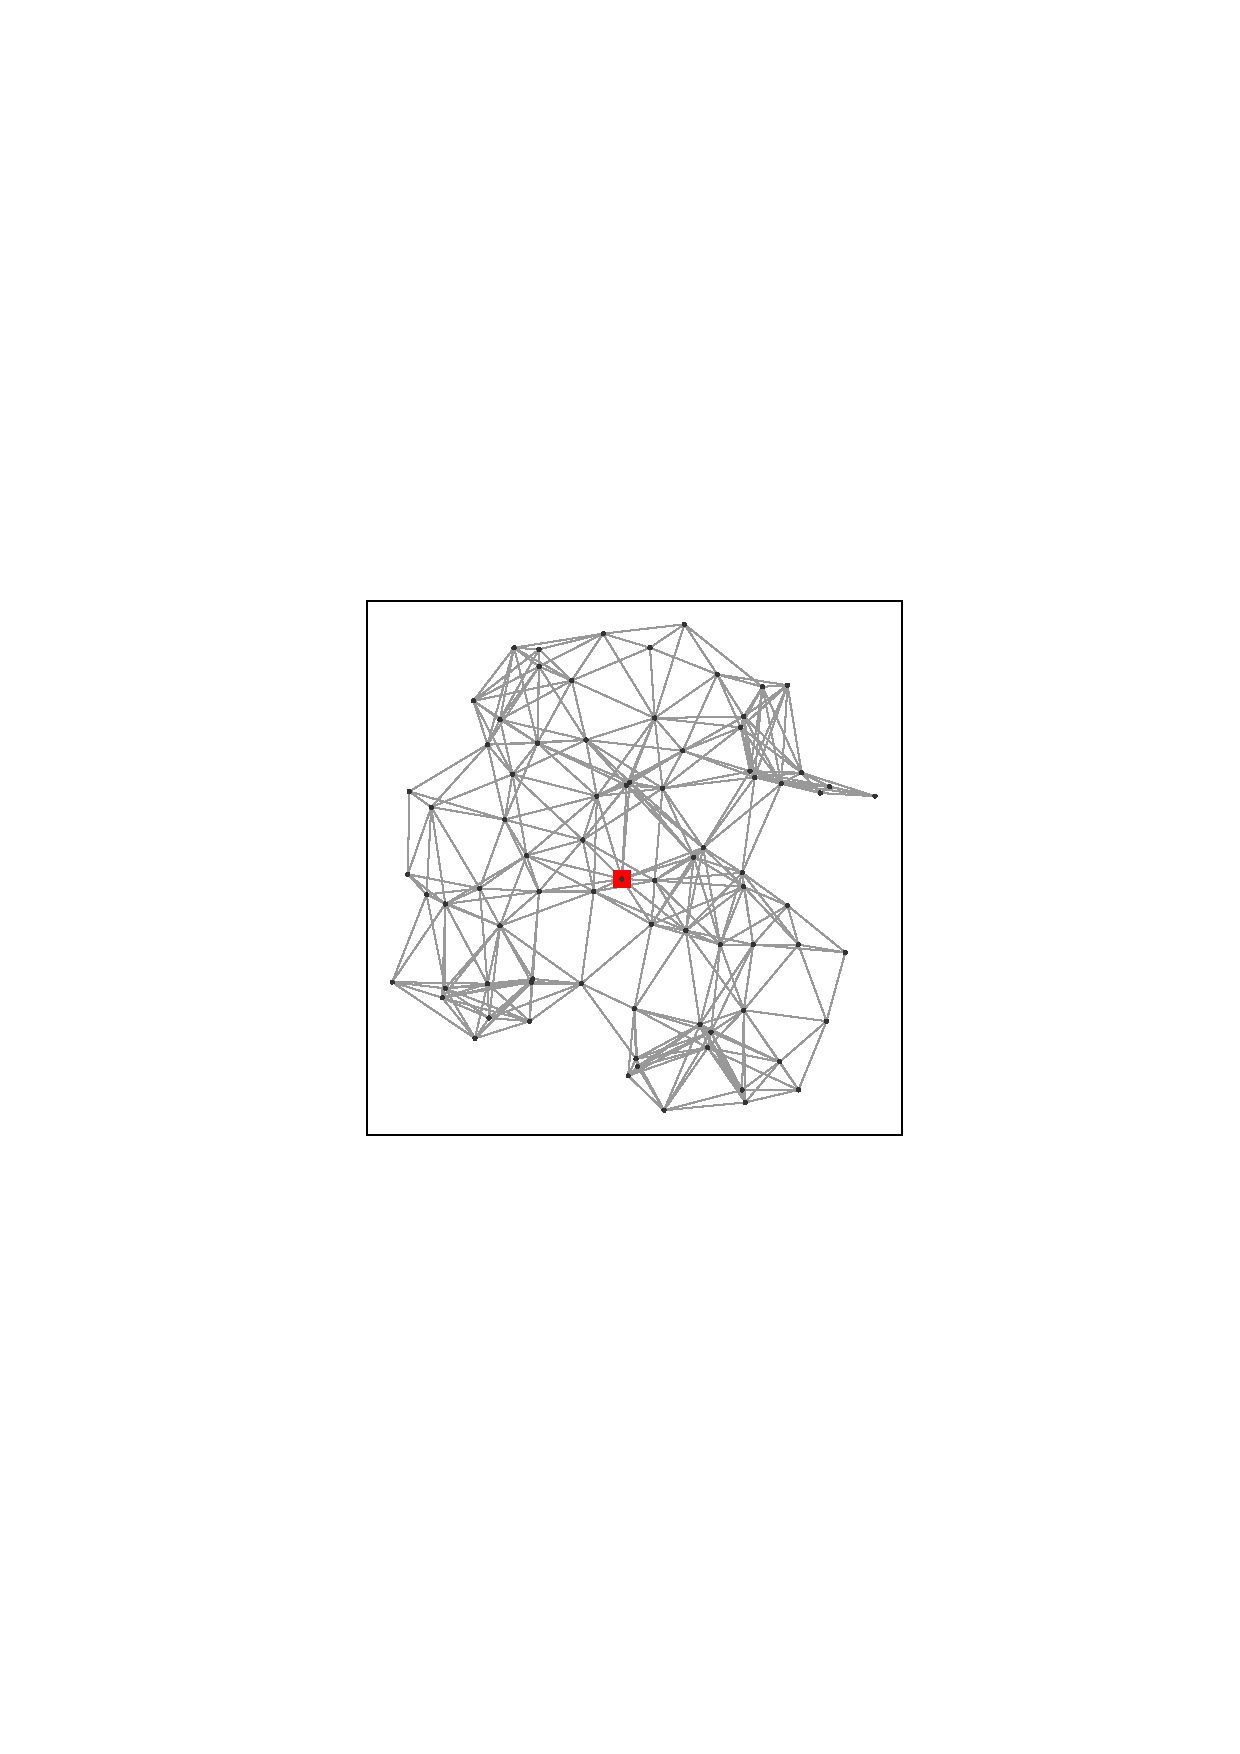
\includegraphics[width=.3\textwidth]{fig302-b}}\hspace{0.25em}%
  \subfloat[内部节点的嵌入结果]{
    \label{fig:302c}
    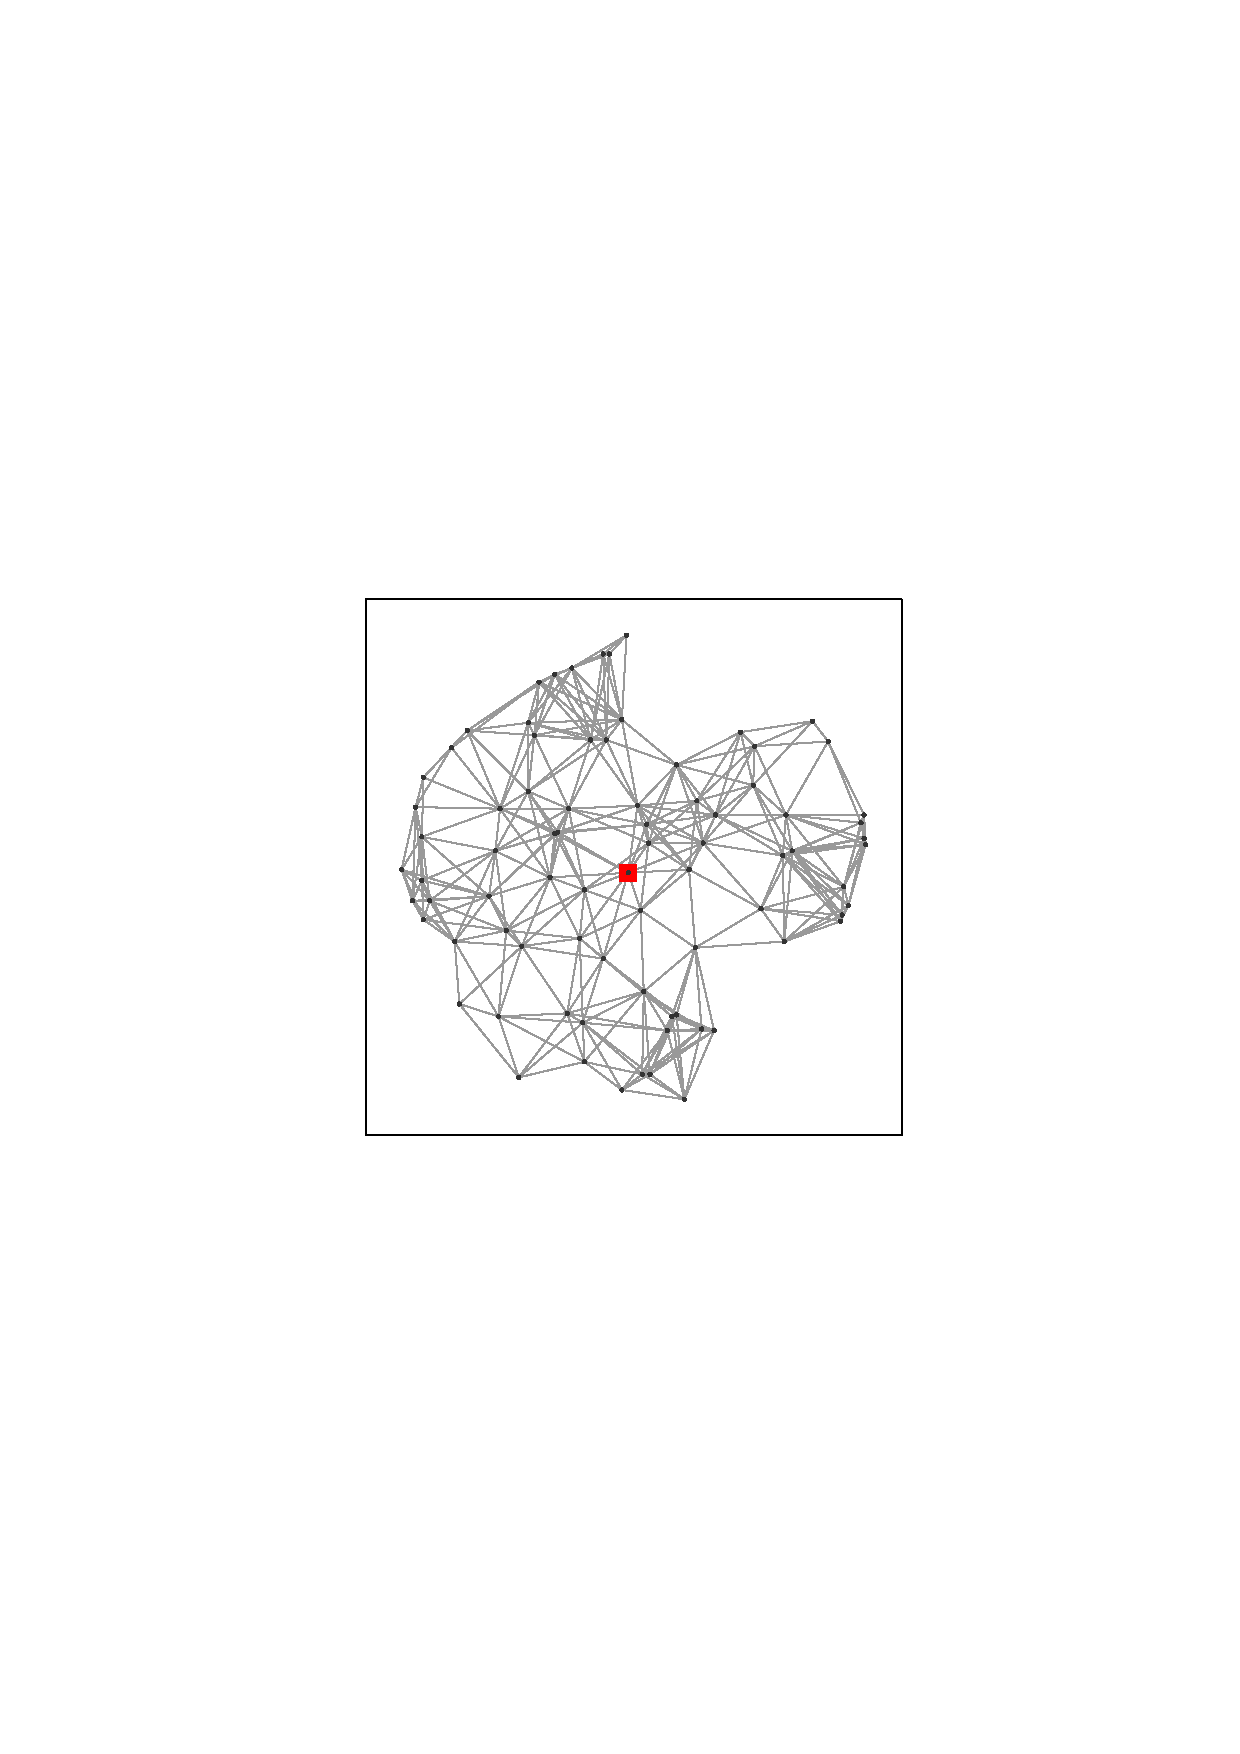
\includegraphics[width=.3\textwidth]{fig302-c}}\hspace{0.25em}%
  \subfloat[边界节点的局部连通图]{
    \label{fig:302d}
    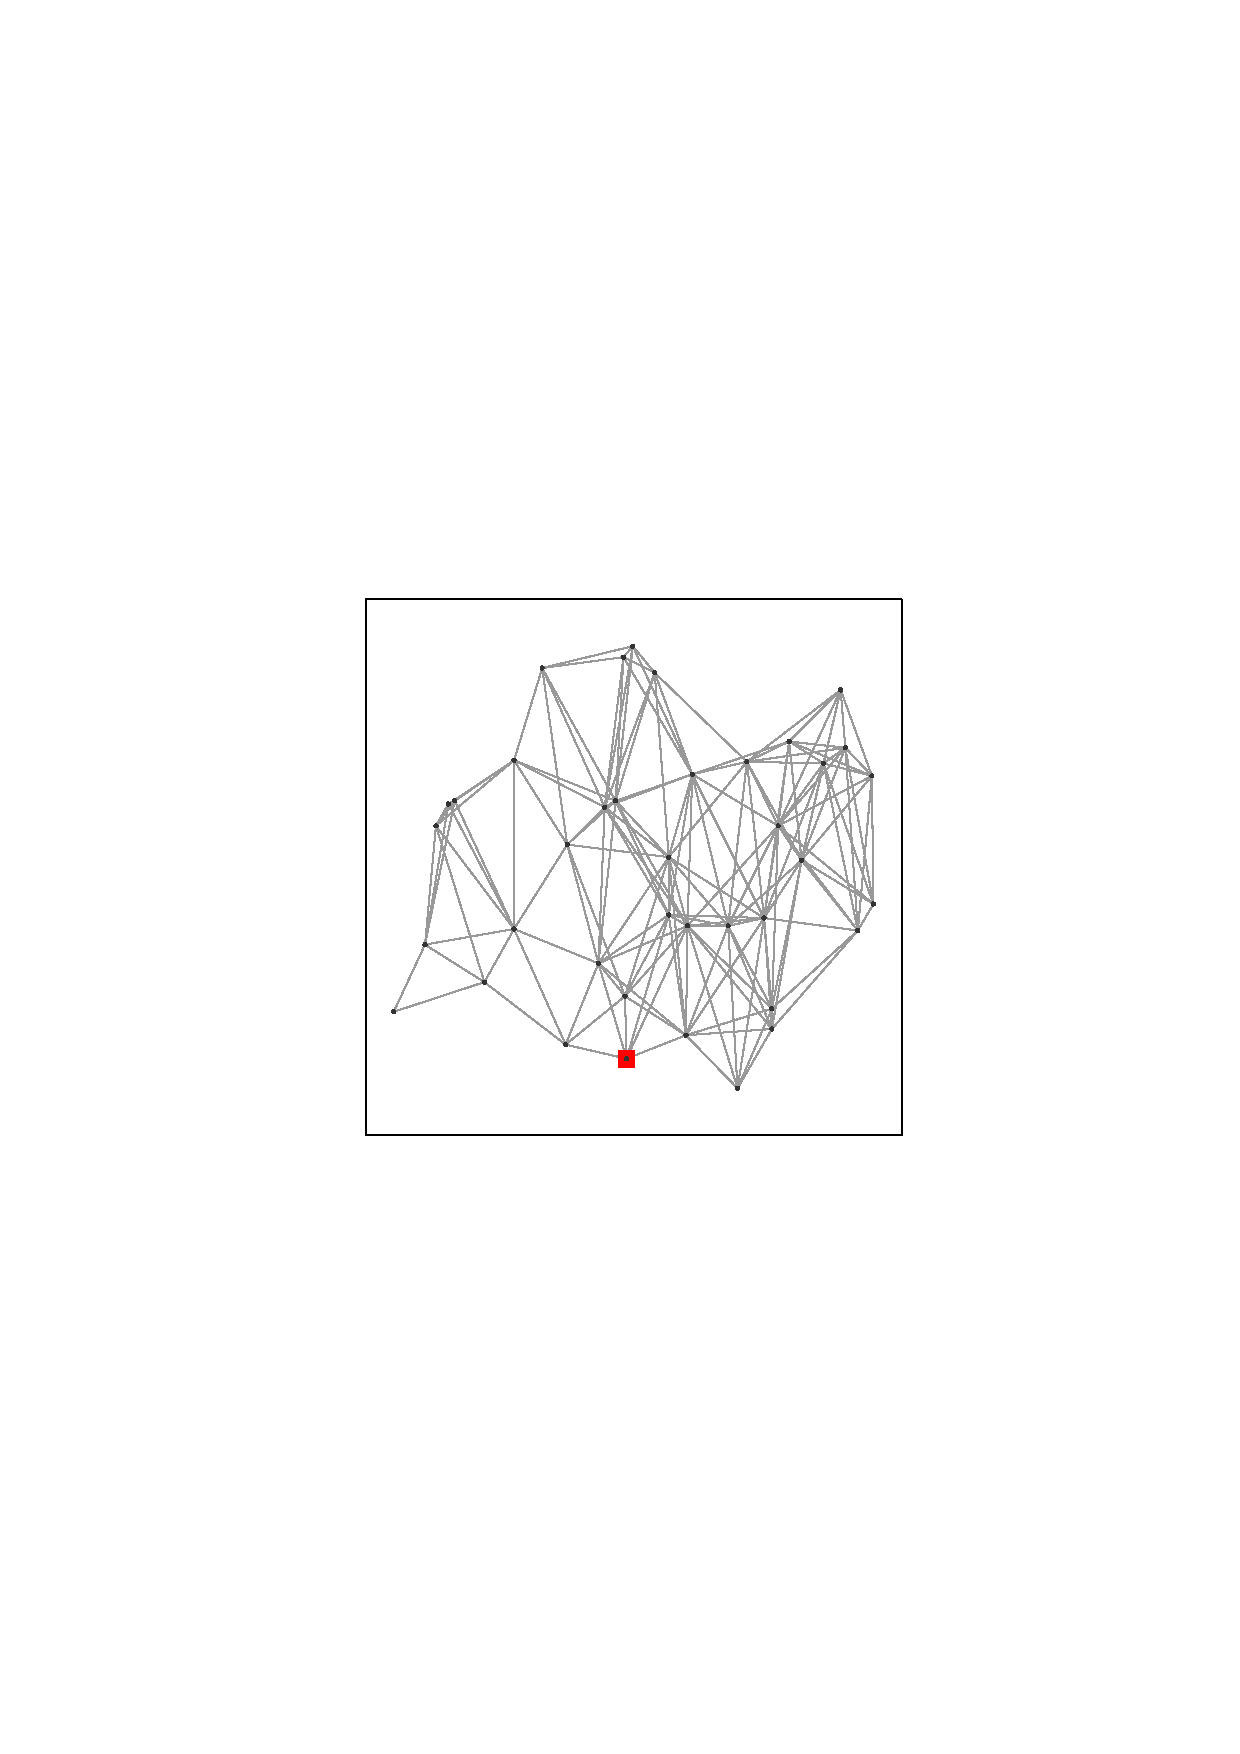
\includegraphics[width=.3\textwidth]{fig302-d}}\hspace{0.25em}%
  \subfloat[边界节点的嵌入结果]{
    \label{fig:302e}
    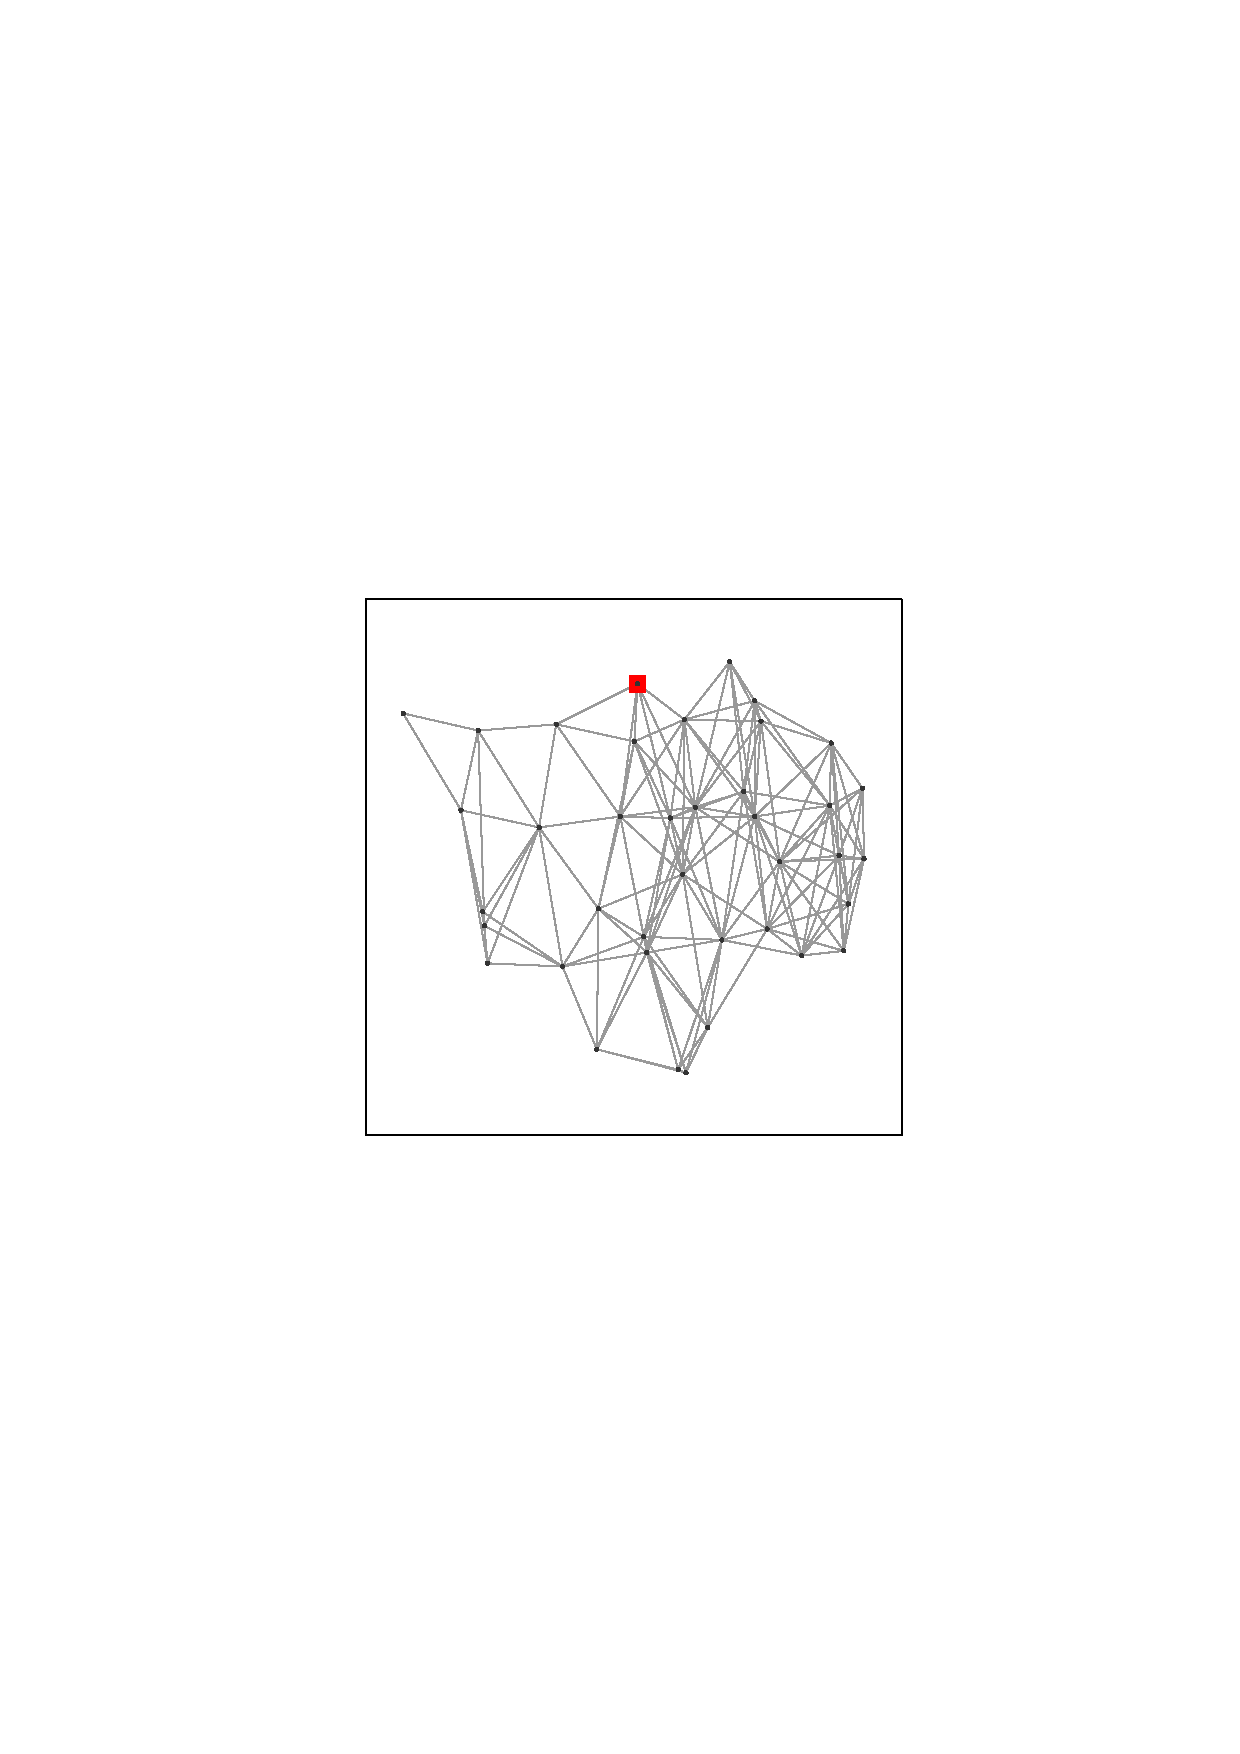
\includegraphics[width=.3\textwidth]{fig302-e}}\hspace{0.25em}%
  \subfloat[边界节点识别结果]{
    \label{fig:302f}
    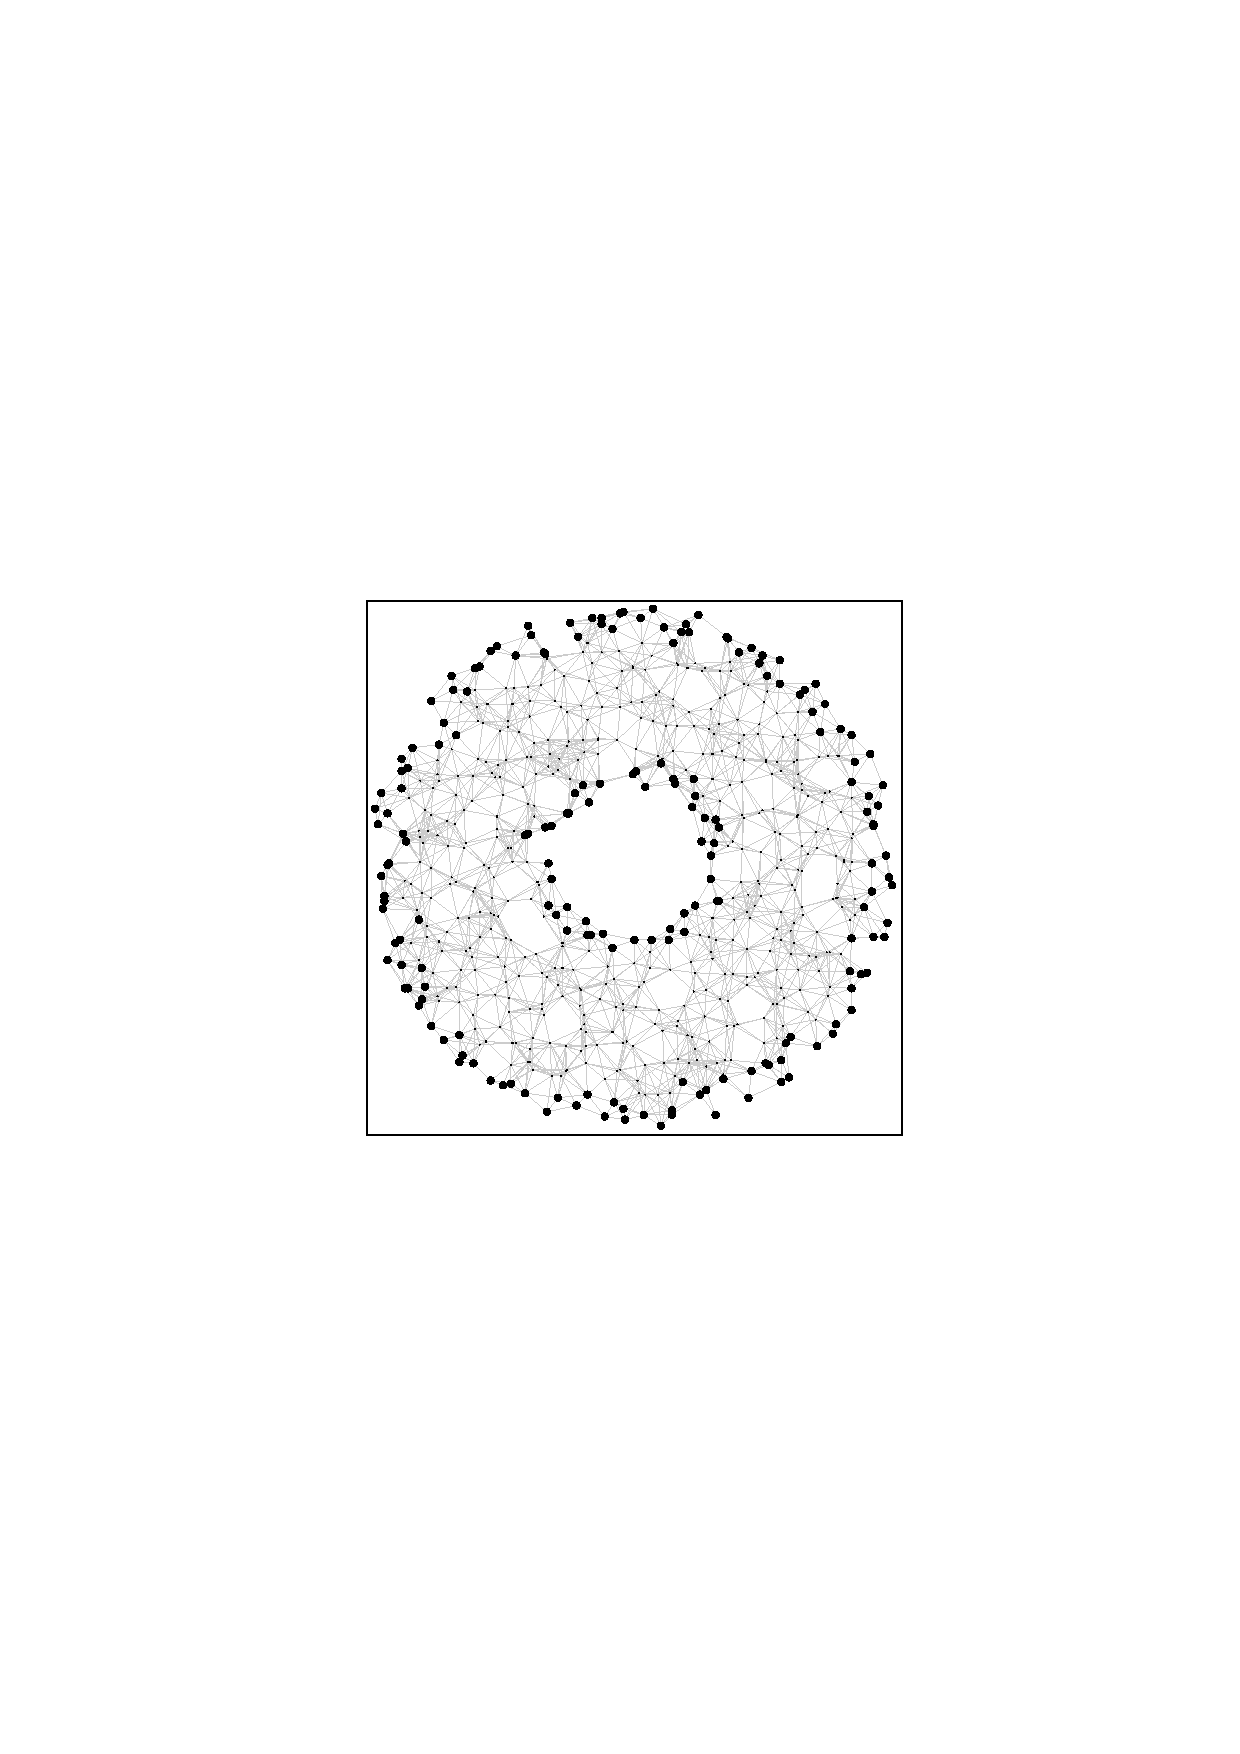
\includegraphics[width=.3\textwidth]{fig302-f}}
  \caption{基于MDS的边界识别过程}
  \label{fig:302}
\end{figure}

下面用图\ref{fig:302}中的实例来直观地说明MDS边界识别算法的原理和过程。对于图\ref{fig:302a}中所示的网络连通图,我们任意选定两个分别位于网络边界和网络内部的节点。然后,两个节点分别收集自身的3跳邻居信息,得到局部连通图(即局部邻居子图)。例如,图\ref{fig:302b}和图\ref{fig:302d}分别给出了两个节点的3跳邻居子图。这里需要强调的是,为了更直观地进行比较,图中利用了节点的实际坐标信息,但是实际上算法在执行过程中并不需要利用任何实际的坐标信息。接下来,节点计算邻居子图中所有节点对之间的最短跳数距离,得到一个跳数距离矩阵。然后以该跳数距离矩阵为输入调用MDS算法,将局部连通图嵌入到平面上,为每个节点分配虚拟坐标,并使节点虚拟坐标之间的欧式距离尽量接近它们在连通图中的跳数距离。图\ref{fig:302c}和图\ref{fig:302e}分别表示图\ref{fig:302b}和图\ref{fig:302d}中局部连通图的MDS嵌入结果。从图中可以直观地看出,MDS嵌入后节点之间的位置关系与它们在真实网络中的分布情况非常接近,嵌入得到的虚拟网络图基本上是实际网络图的反转和镜像。因此,我们可以利用嵌入后的节点坐标信息来近似地判断它们在原始网络中的位置,并进行边界节点的判定。基于位置的边界检测方法比较简单。图\ref{fig:303}给出了利用位置信息进行边界检测的简单示例,其中粗线表示实际的网络边界。当节点的局部邻居与本节点之间的边形成的夹角的最大值超过某个设定的门限值时,就判定该节点为边界节点。基于以上原理,我们利用MDS技术对图\ref{fig:302a}中所示的网络连通图进行处理,并利用基于位置的边界检测方法得到了如图\ref{fig:302f}所示的边界识别结果。
\begin{figure}[h]
  \centering
  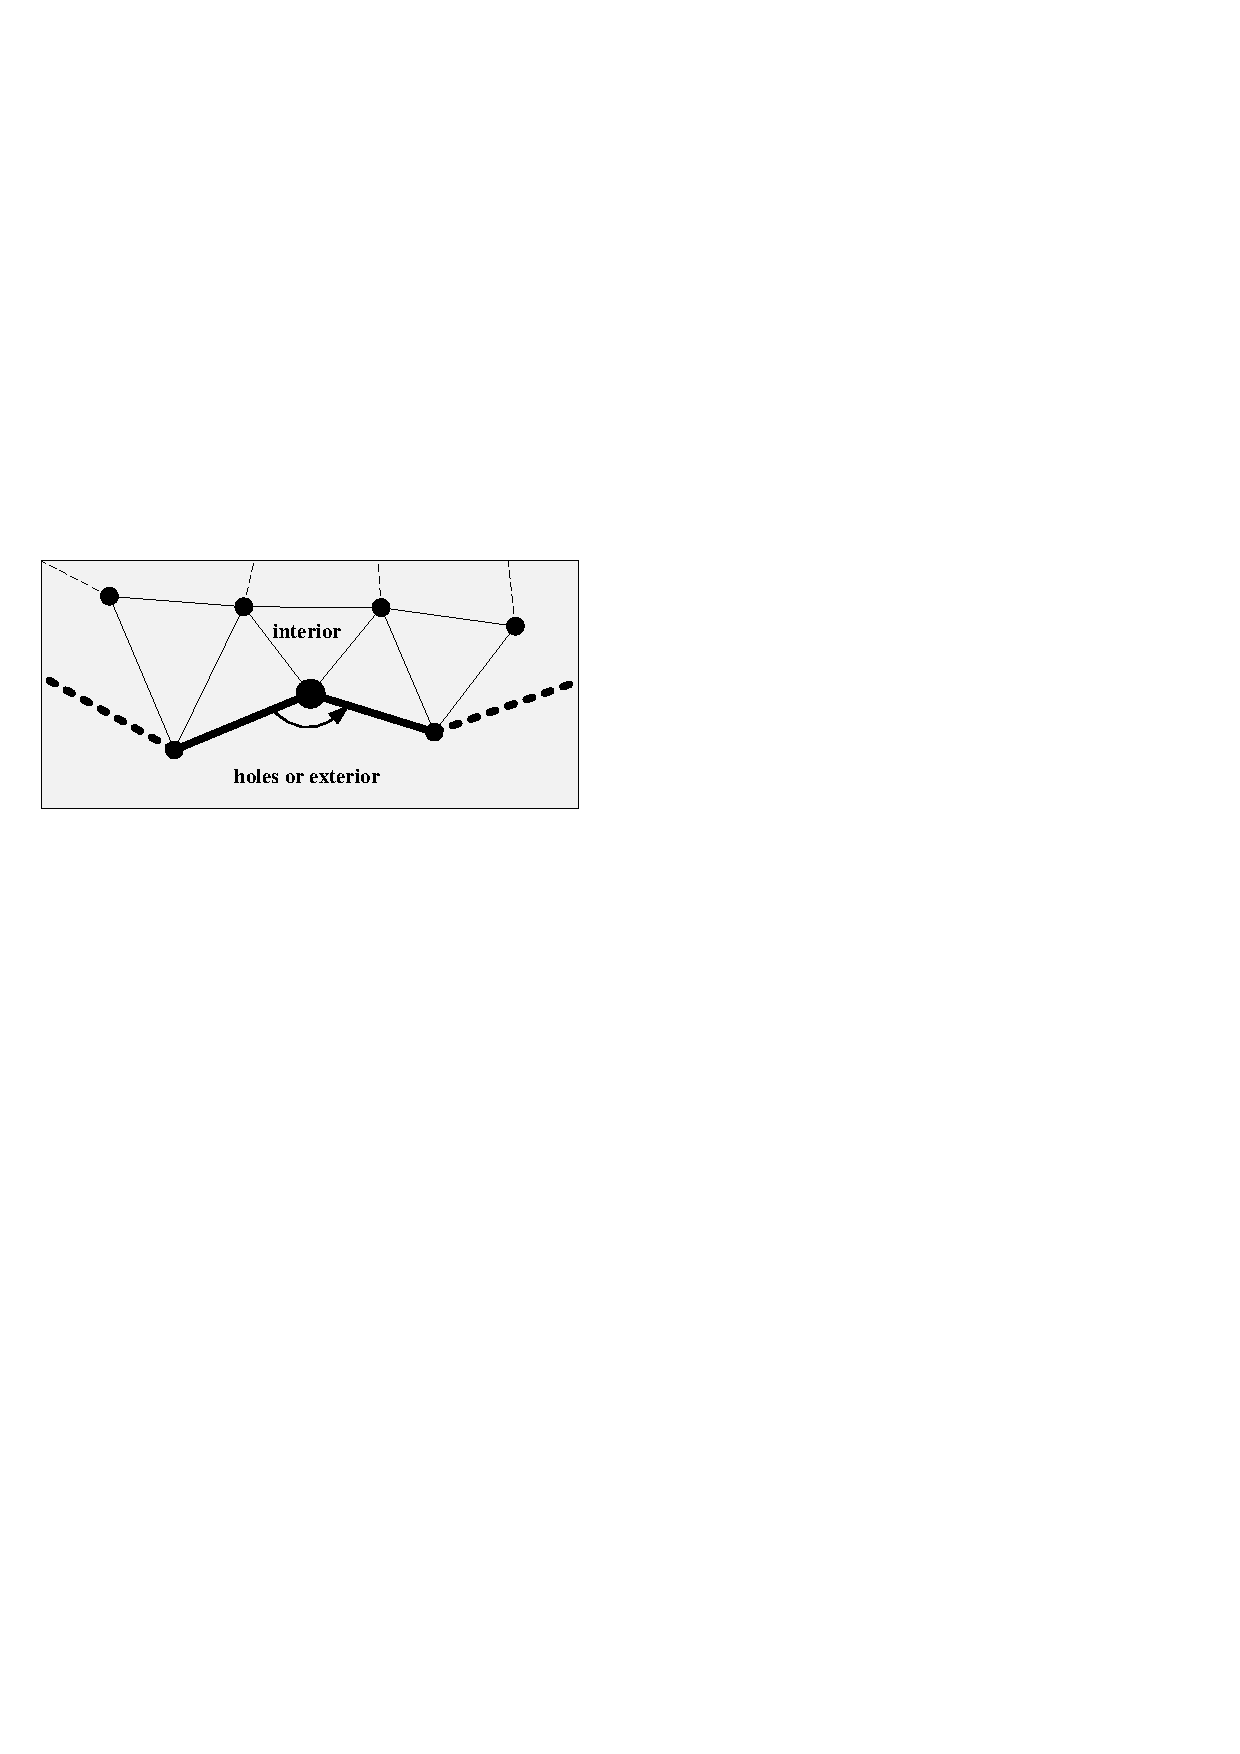
\includegraphics[width=0.4\textwidth]{fig303}
  \caption{基于位置的边界节点检测原理示意图}
  \label{fig:303}
\end{figure}

按照以上的边界识别方法,我们就可以从图\ref{fig:301a}所示的网络连通图$G$中检测出图\ref{fig:301b}所示的一定数量的边界节点,表示为集合$B(G)$。
\subsection{骨干节点提取}
前一个组件从网络中识别出边界节点,本组件将利用这些边界节点信息从网络中提取出一定数量的骨干节点。

首先找出由边界节点构成的所有连通分支,这些连通分支构成了图$G$的边界分支集合,记为$\mathcal{C}$。图\ref{fig:301c}所示为图\ref{fig:301b}中所示的边界节点组成的三个边界分支。对于网络中的任意两个节点$u,v$和任意一个边界分支$C_i\in{\mathcal{C}}$,设$d(u,v)$表示点$u,v$之间的距离,即最短路径长度,设$D(v,C_i)$表示节点$v$到边界分支$C_i$的距离,其中$D(v,C_i)=min(d(v,w),w\in{C_i})$,即点$v$到分支$C_i$上所有节点的距离的最小值。对于网络中的任意一个节点,如果该节点到两个或两个以上最近的边界分支的距离相等,则将该节点标记为骨干节点。该判断准则的原理非常简单:从直观上来看,对于存在多条边界分支的网络,每个骨干节点都应该位于至少两条边界的中间位置。下面描述该过程的实现细节。首先对每个边界节点进行如下的命名,$<C_i,ID_j>$表示边界分支$C_i$中ID为$ID_j$的节点。每个边界节点向网络中发送一个包含自身名字的简单的洪泛消息,该洪泛消息中包含一个代表消息转发次数的计数器。每个内部节点记录下来自每个边界分支的洪泛消息中包含的计数器的最小值,作为该节点到该边界分支的最短距离。洪泛消息完成后,每个节点就可以获得自身到所有的边界分支的距离。

但是,仅采用以上的原则来判定骨干节点存在如下的缺陷:第一,如果网络中仅存在一条独立的边界分支,例如在没有内部边界的网络,且边界节点被很好地识别成唯一的连通分支,则以上判定准则失效;第二,以上判断准则并不能很好地应用于所有的网络中,例如在稀疏部署的网络中仅有少量的节点被识别成骨干节点\upcite{skeleton_tpds10}。为了克服这一缺陷,我们又引入了另外一种骨干节点的判定准则,即骨干节点到边界的距离局部最大化原则。一般情况下,骨干节点位于网络的中央位置,因此骨干节点比其它节点距离边界更远。因此,对于任意节点$v$的$\delta$跳以内的邻居集合$N_G^{\delta}(v)$,如果满足条件$D(v,B(G))>=D(N_G^{\delta}(v),B(G))$,则节点$v$被标记为骨干节点。这里需要指出的是,并非所有的骨干节点到网络边界的最短距离都是局部最大的,例如相邻的两个骨干节点到边界的最小距离可能是不相等的。但是大多数情况下,相邻的骨干节点到边界的距离应该是趋于相等的,因此利用该原则仍然能够从网络中提取出一定数量的骨干节点。在之前的过程中,我们已经得到了每个节点到网络中所有边界分支的距离,因此可以很容易得到每个节点到网络边界的最小距离。
\begin{figure}[h]
  \centering
  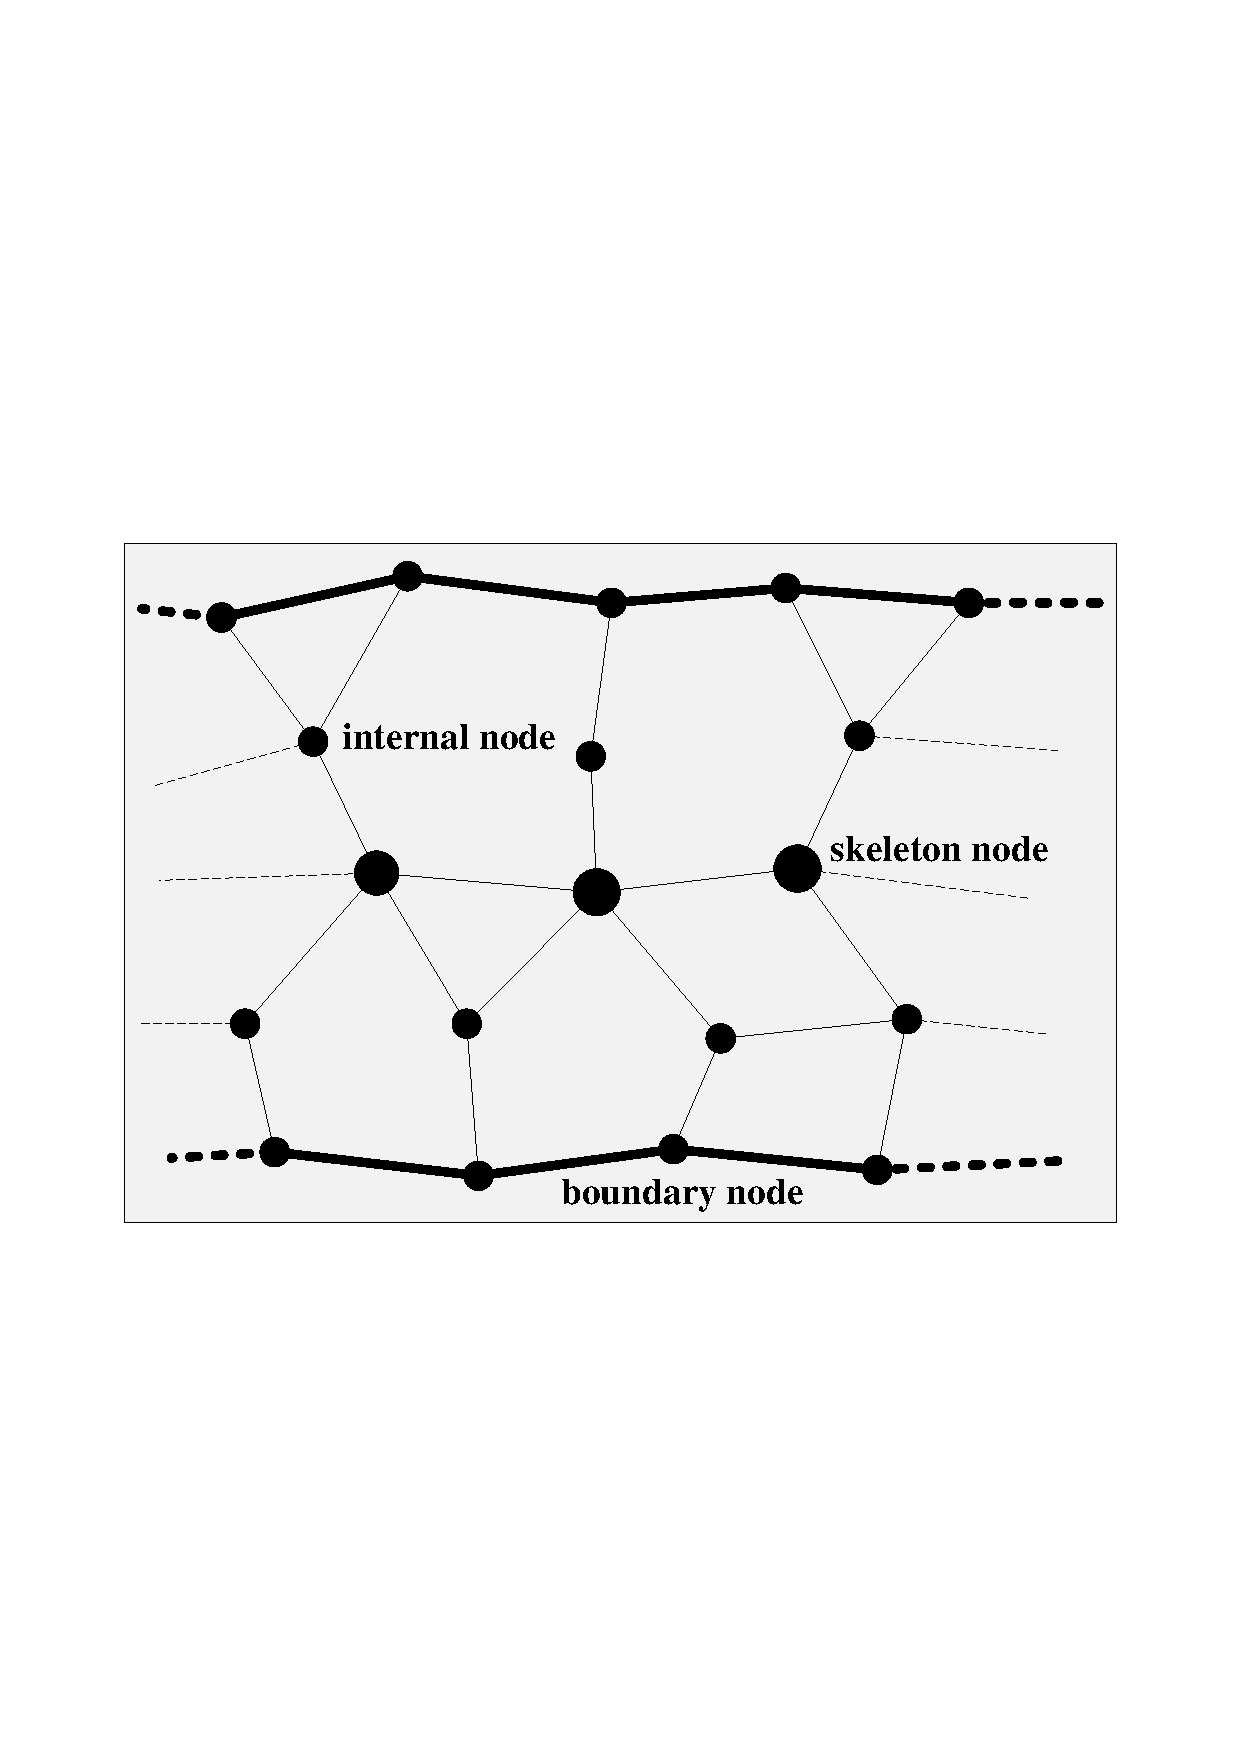
\includegraphics[width=0.4\textwidth]{fig304}
  \caption{骨干节点的判定原则示意图}
  \label{fig:304}
\end{figure}

图\ref{fig:304}给出了骨干节点在网络中的分布情况的简单示例,其中粗实线表示网络边界,比较大的点表示骨干节点。可见,每个骨干节点到两条边界的最短距离都是2跳,而每个骨干节点到边界的最短距离也都是局部最大化的。按照如上的两条原则,我们给出了骨干节点的形式化的定义,如定义\ref{def:301}所述。
\begin{definition}\label{def:301}
给定网络连通图$G$以及网络中任意的一个节点$v$,如果节点$v$满足如下两个条件中的任意一个,则$v$为骨干节点:(1)$G$中存在两条或两条以上的边界分支$C_i,...,C_j$,满足节点$v$到这些边界分支的距离最小且相等,即$D(v,C_i)=...=D(v,C_j)=\min{D(v,B(G))}$;(2)对于节点$v$和它的$\delta$跳以内的邻居集合$N_G^k(v)$,满足$v$到$G$的边界节点集合$B(G)$的距离是局部最大的,即$D(v,B(G))\ge{D(N_G^k(v),B(G))}$。
\end{definition}

按照骨干节点的定义方式,我们就可以从网络中提取出图\ref{fig:301d}所示的一定数量的骨干节点,表示为集合$S(G)$。
\subsection{原始骨干提取}
前一个组件提取出一定数量的骨干节点之后,本组件利用这些骨干节点信息从网络中提取出初始的骨干网络。

一般情况下,前一个组件中提取出的骨干节点往往无法形成唯一的连通分支,而是被分割成多个连通分支。首先,我们找出网络中由骨干节点组成的所有的连通分支集合,表示为$\mathcal{S}$。然后,本组件通过两个简单的步骤对骨干节点进行扩展,以改善它们之间的连通性。第一步将骨干节点扩展为唯一的连通分支。该过程的实现方式如下:对于每一条骨干节点连通分支,分别将它们与距离自身最近的骨干节点连通分支连接起来。具体来讲,对于任意一个骨干节点连通分支$S_i$,首先找出距离最近的骨干节点连通分支$S_j$,以及二者之间距离最近的节点对$u,v$,其中$u\in{S_i},v\in{S_j}$。然后找出节点对$u,v$之间的一条最短路径$P_{u,v}$,将该路径中所有节点加入骨干节点集合$S(G)$中。该过程迭代地执行,直到所有的骨干节点形成唯一的连通分支,如图\ref{fig:301e}所示。第二步,将骨干节点进一步地扩展成骨干带网络。该过程是通过将所有的骨干节点扩展至$\tau$跳邻居来实现。具体来讲,每个骨干节点找出自己的$\tau$跳以内的邻居节点,并将其加入骨干节点集合$S(G)$中。此时,所有的骨干节点以及它们之间的边构成了一个具有良好连通性且形状与网络的全局形状一致的骨干带网络,表示为$\Gamma_{S(G)}$。一般情况下,$\tau$仅需设置为一个极小的常数,如图\ref{fig:301f}所示为$\tau=1$时得到的骨干带网络。

接下来,我们设计一种图变换工具HPT,对骨干带网络进行处理,从中抽取出一个初始骨干。在介绍HPT变换工具之前,首先给出一些基本的概念。设$G$是以$V(G)$为顶点集、以$E(G)$为边集的简单图。图$G$中的环$C$为一个节点度均为2的连通子图。环$C$可以表示为$G$中边的索引向量$b(C)=(b_1,b_2,...,b_i,...)$,其中$i\in{[1,|E(G)|]}$,且$b_i=1$当且仅当$e_i\in{E(C)}$,$b_i=0$当且仅当$e_i\notin{E(C)}$。环$C$的长度$|C|$定义为其包含的边的数量$|E(C)|$。所有环的索引向量张成$\{0,1\}$二元域上的向量空间,称为图$G$的环空间,记为$\mathcal{C}_G$。环空间中两个环$C_1$和$C_2$的加运算定义为它们的索引向量的模2加,即$C_1\oplus{C_2}=(E(C_1)\cup{E(C_2)})\setminus{E(C_1)\cap{E(C_2)})}$。图$G$的环基$\mathcal{Q}$是环空间$\mathcal{C}_G$的一组向量基。环基$\mathcal{Q}$ 的长度$l(\mathcal{Q})$定义为其中所有环的长度之和,即$l(\mathcal{Q})=\sum_{C\in{\mathcal{Q}}}|C|$。有了环基的概念,我们就可以用来定义单连通图。如果图$G$具有仅由三角形构成的环基,则$G$为单连通图。例如,边、三角形、树结构都是单连通图,而四边形不是单连通图。利用单连通图的概念,定义\ref{def:302}给出了HPT变换的具体定义。
\begin{definition}\label{def:302}
给定图$G(V,E)$,图$G$上的HPT变换是一系列图操作的集合,包括如下定义的点删除和边删除操作:
\begin{itemize}
\item 点删除:设$v$是$G$中一个顶点,$v\in{V}$,$v$可以从$G$中删除以获得新图$G^{'}=G(V\setminus\{v\})$,如果满足以下两个条件:(1)$v$的1跳邻居子图$G(v)$是连通的;(2)存在单连通图$G^{''}\subseteq{G^{'}}$,使得$G_1(v)\subseteq{G^{''}}$。
\item 边删除:设$e$是$G$中一条边,$e\in{E}$,$e$可以从$G$中删除以获得新图$G^{'}=G-e$,如果满足以下两个条件:(1)$e$的1跳邻居子图$G(e)$是连通的;(2)存在单连通图$G^{''}\subseteq{G^{'}}$,使得$G(e)\subseteq{G^{''}}$。
\end{itemize}
\end{definition}

下面利用HPT变换工具对骨干带网络$\Gamma_{S(G)}$进行处理。首先仅考虑初始网络中存在内边界的情况,即如图\ref{fig:301f}所示骨干带网络是封闭的情况。第一步执行点删除过程,在骨干带网络中极大地应用HPT变换的点删除操作得到简化的网络图。每一个节点根据局部的连通性信息确定其是否可以被删除。一般情况下,靠近边界上的点将首先被删除,而内部的节点在关联的边界节点被删除后也将陆续被删除。该过程以迭代的方式进行,算法在每一轮中随机地选择当前图中的一个点,根据HPT 变换判断其是否可以被删除。当没有点可以继续被删除时该过程终止。点删除过程结束后,算法执行边删除操作,以进一步地处理图中可能存在的三角形的环结构。与点删除操作类似,边删除操作仍然是以迭代的方式执行。算法在每一轮中随机地选择当前图中的一条边,根据HPT变换判断其是否可以被删除。当没有边可以继续被删除时该过程终止。此时,我们就可以得到图\ref{fig:301g}中所示的初始骨干,表示为$G_S$。
\begin{figure}[t]
  \centering
  \subfloat[]{
    \label{fig:305a}
    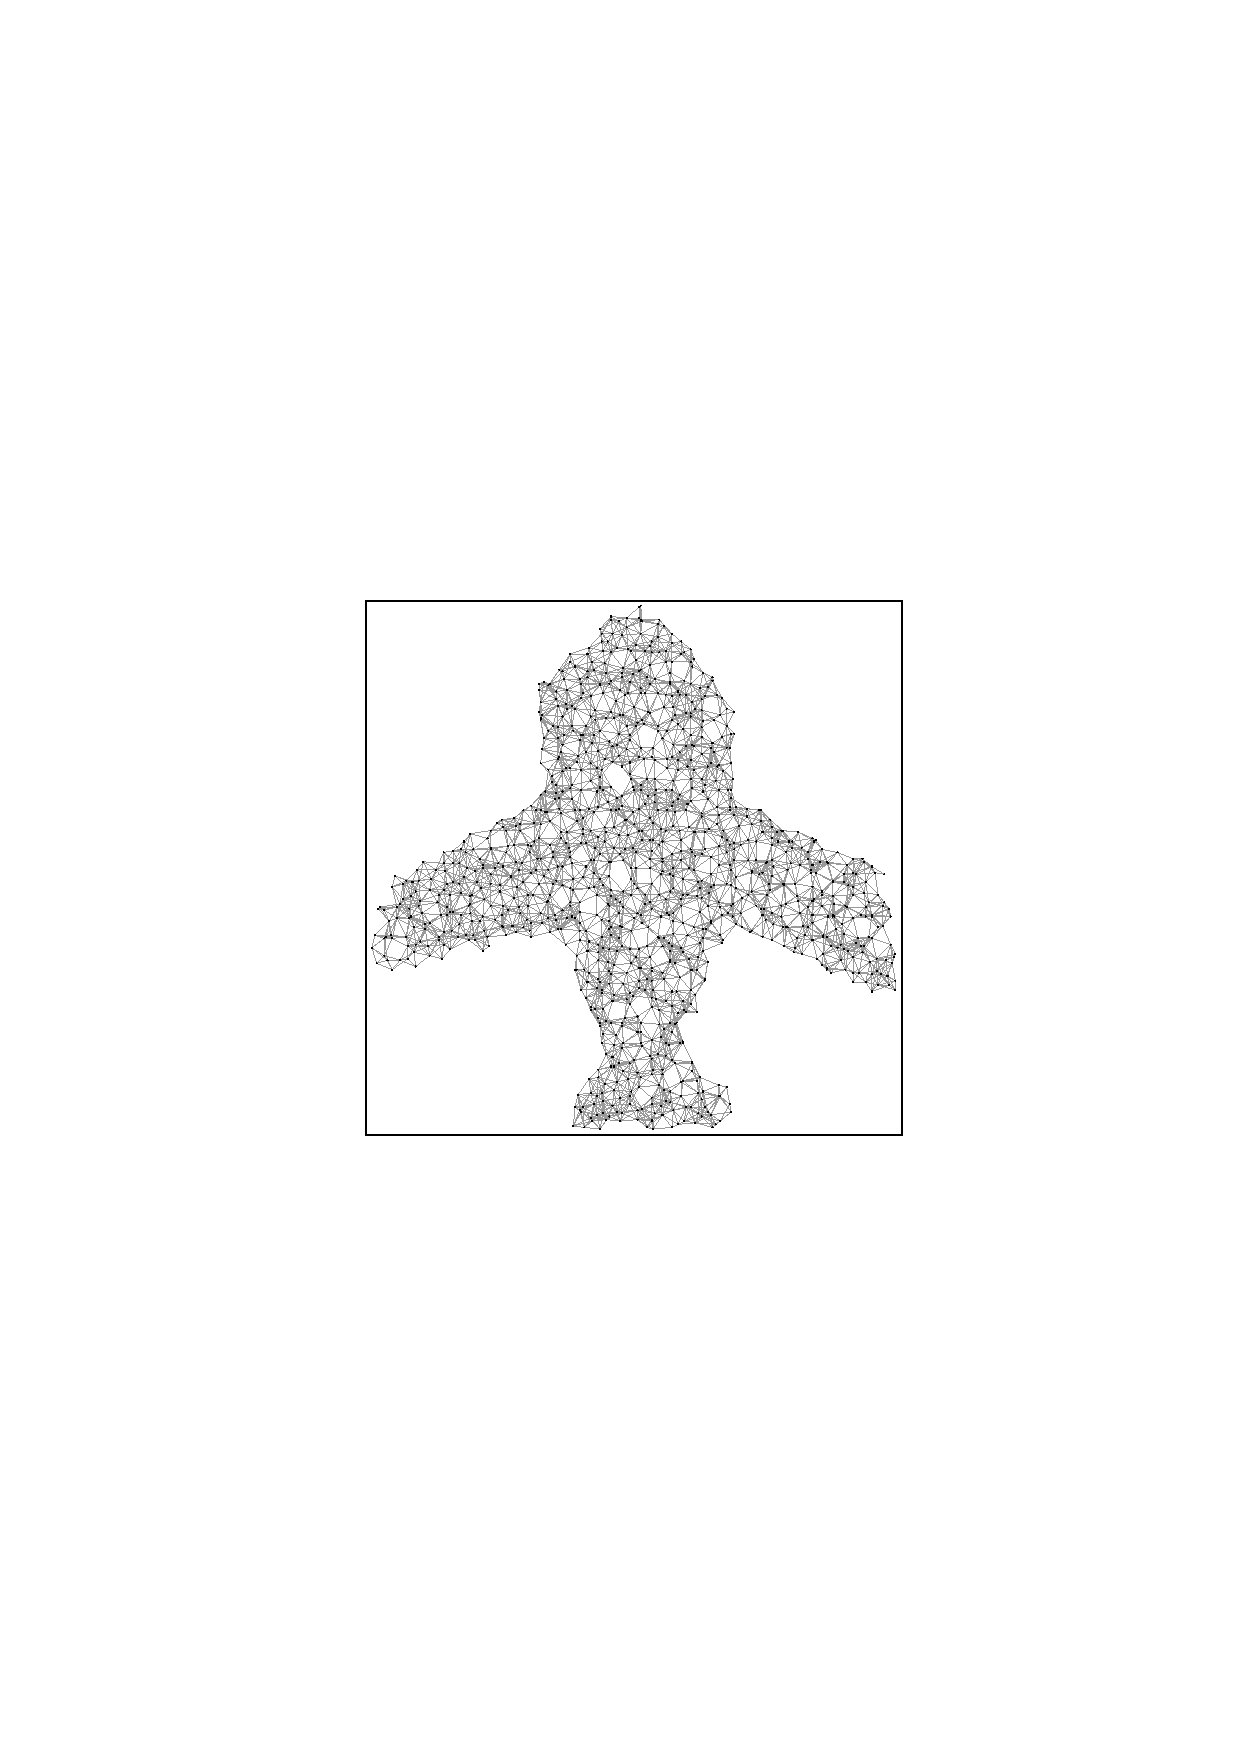
\includegraphics[width=.32\textwidth]{fig305-a}}\hspace{0.25em}%
  \subfloat[]{
    \label{fig:305b}
    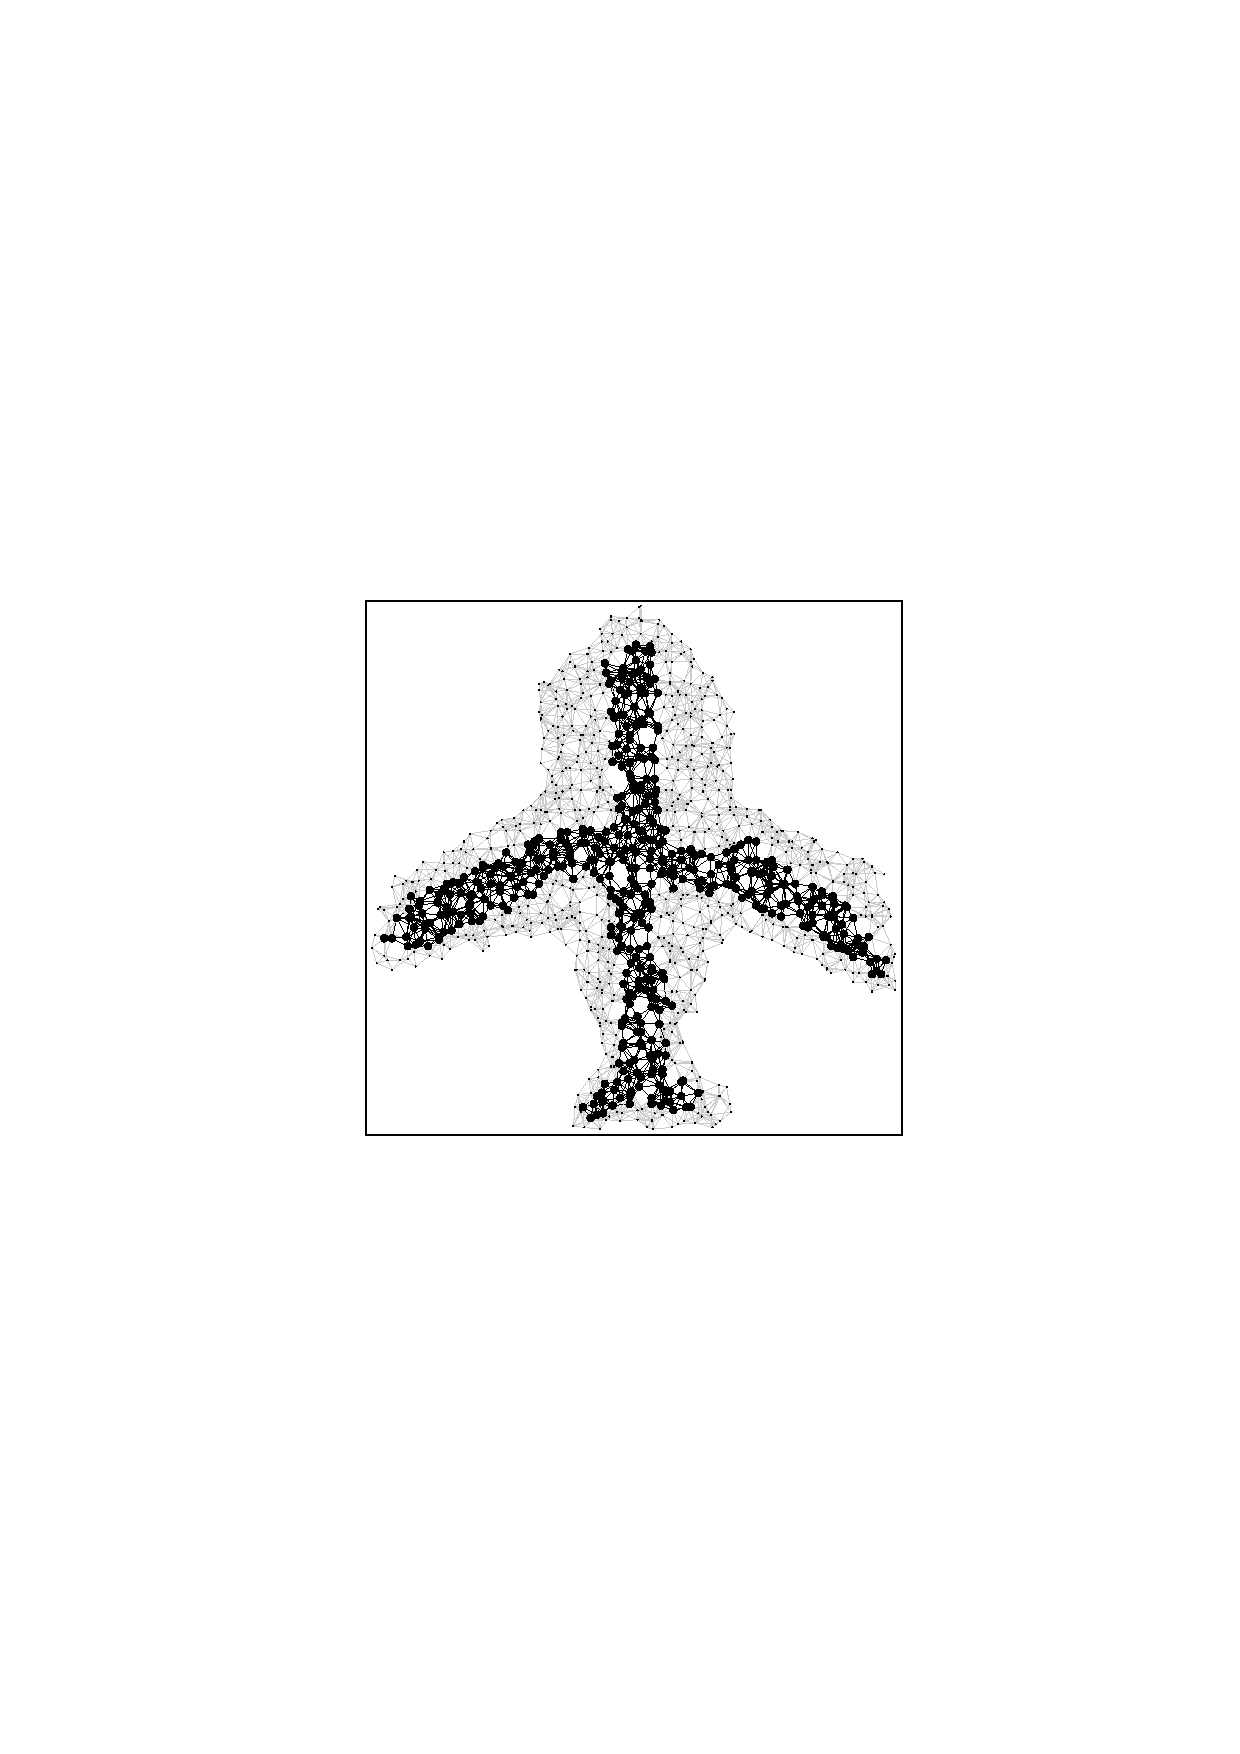
\includegraphics[width=.32\textwidth]{fig305-b}}\hspace{0.25em}%
  \subfloat[]{
    \label{fig:305c}
    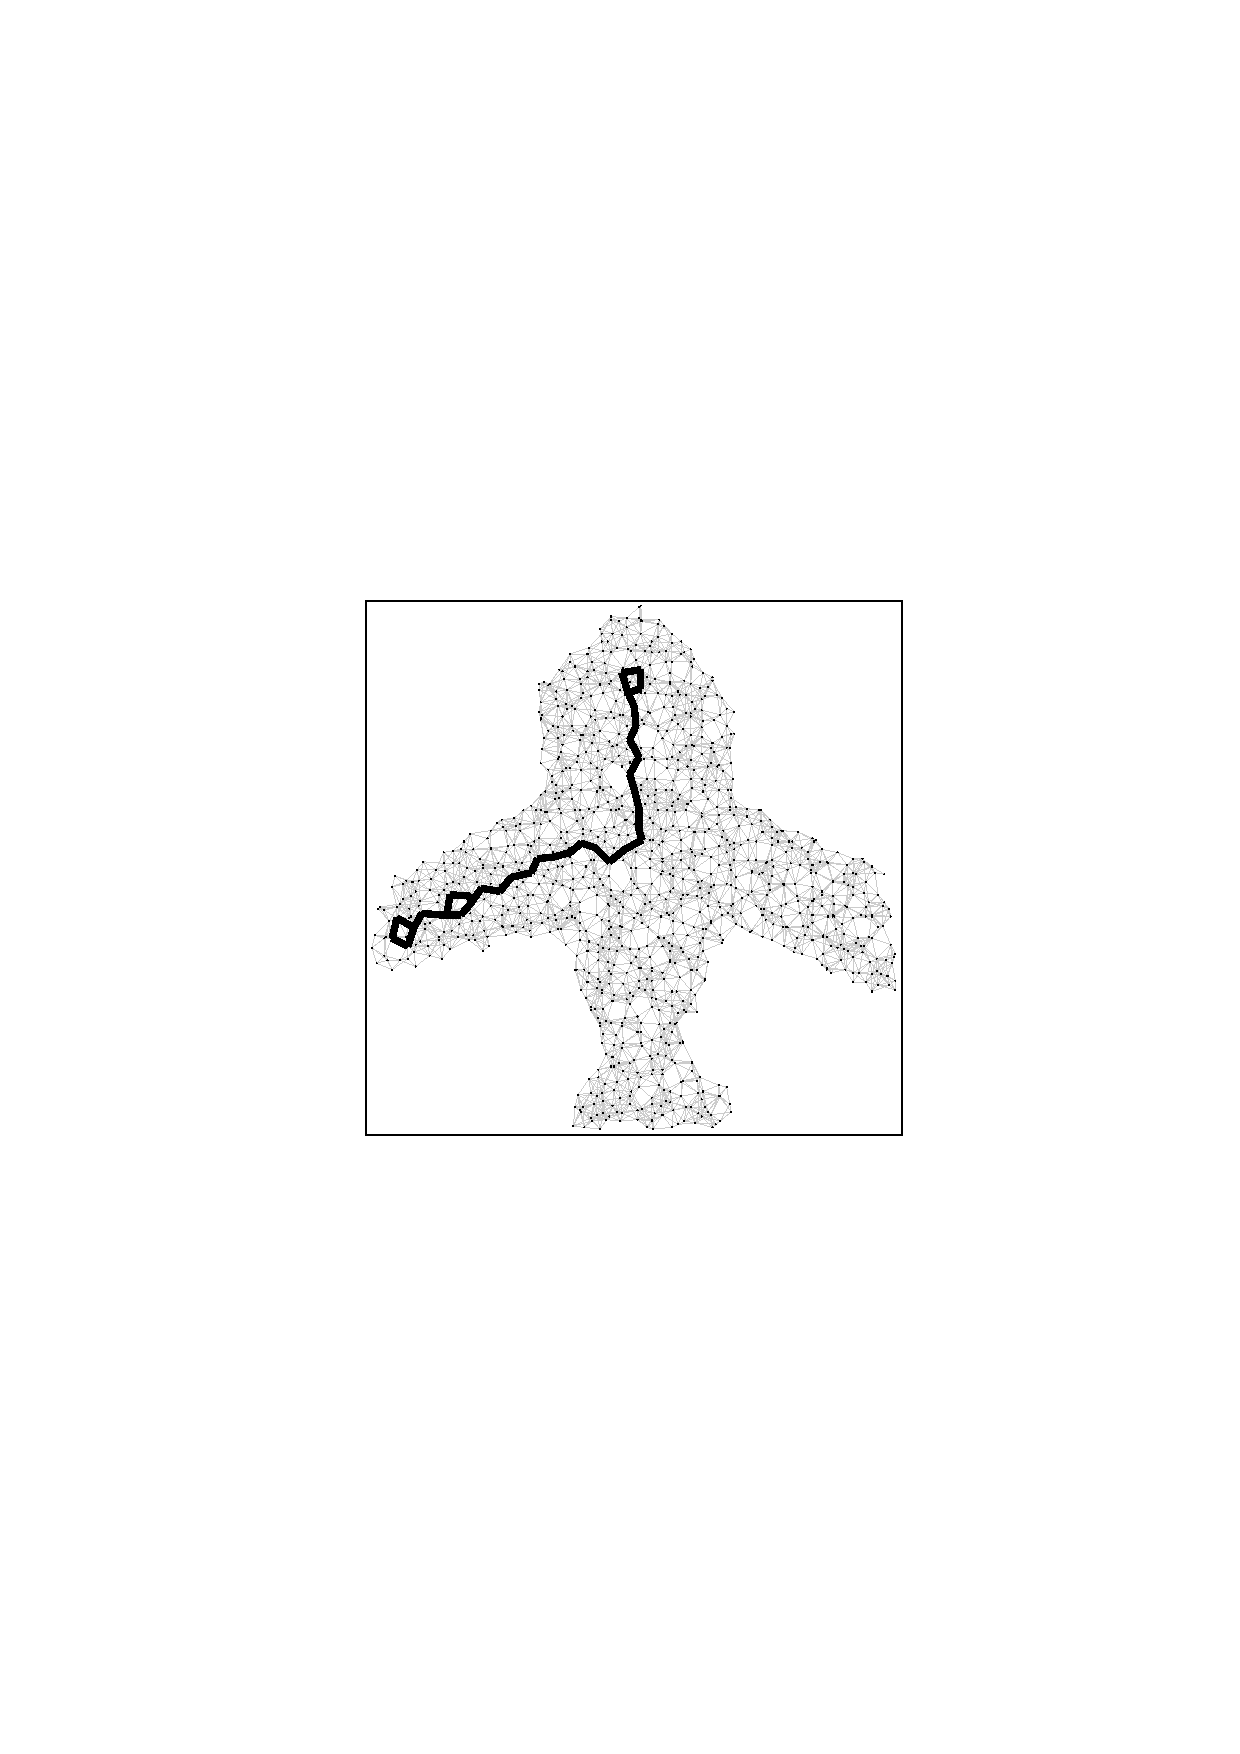
\includegraphics[width=.32\textwidth]{fig305-c}}\hspace{0.25em}%
  \subfloat[]{
    \label{fig:305d}
    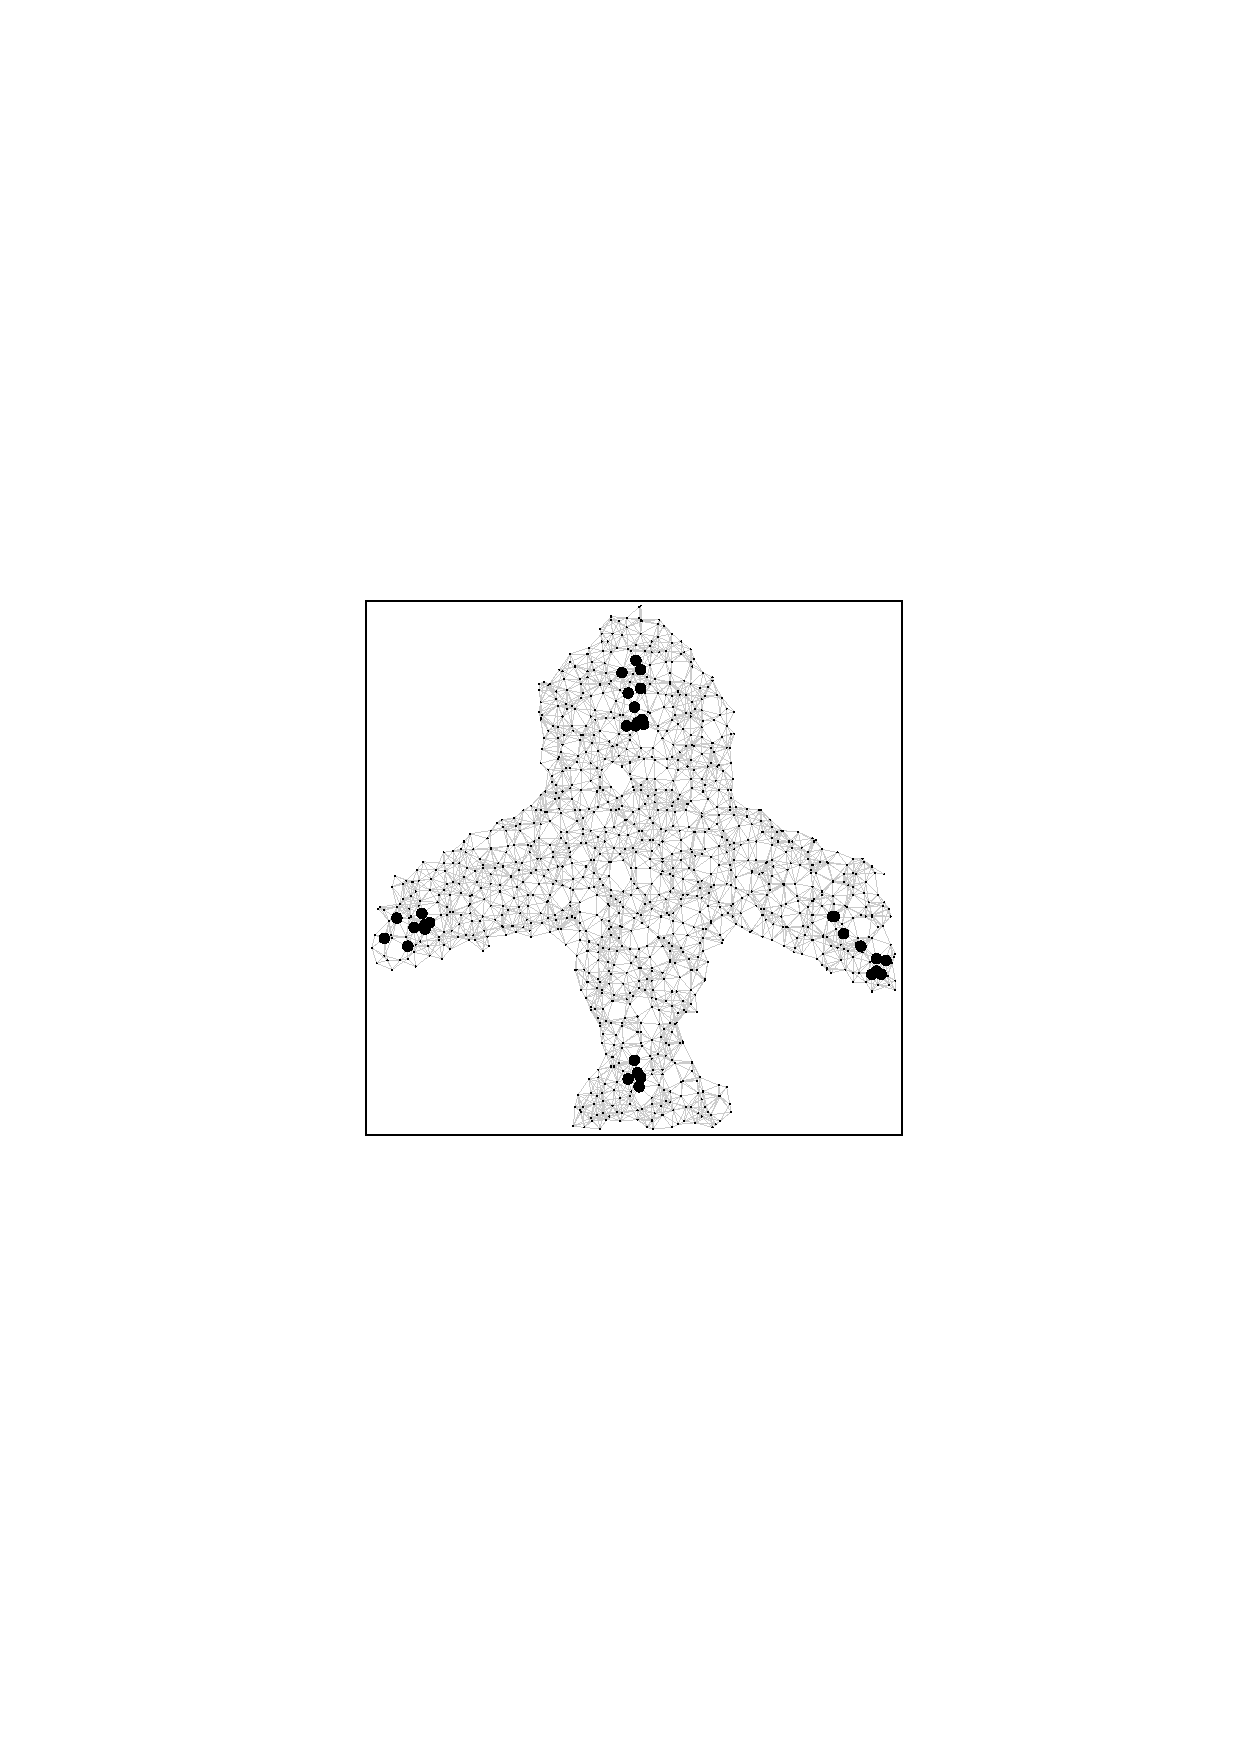
\includegraphics[width=.32\textwidth]{fig305-d}}\hspace{0.25em}%
  \subfloat[]{
    \label{fig:305e}
    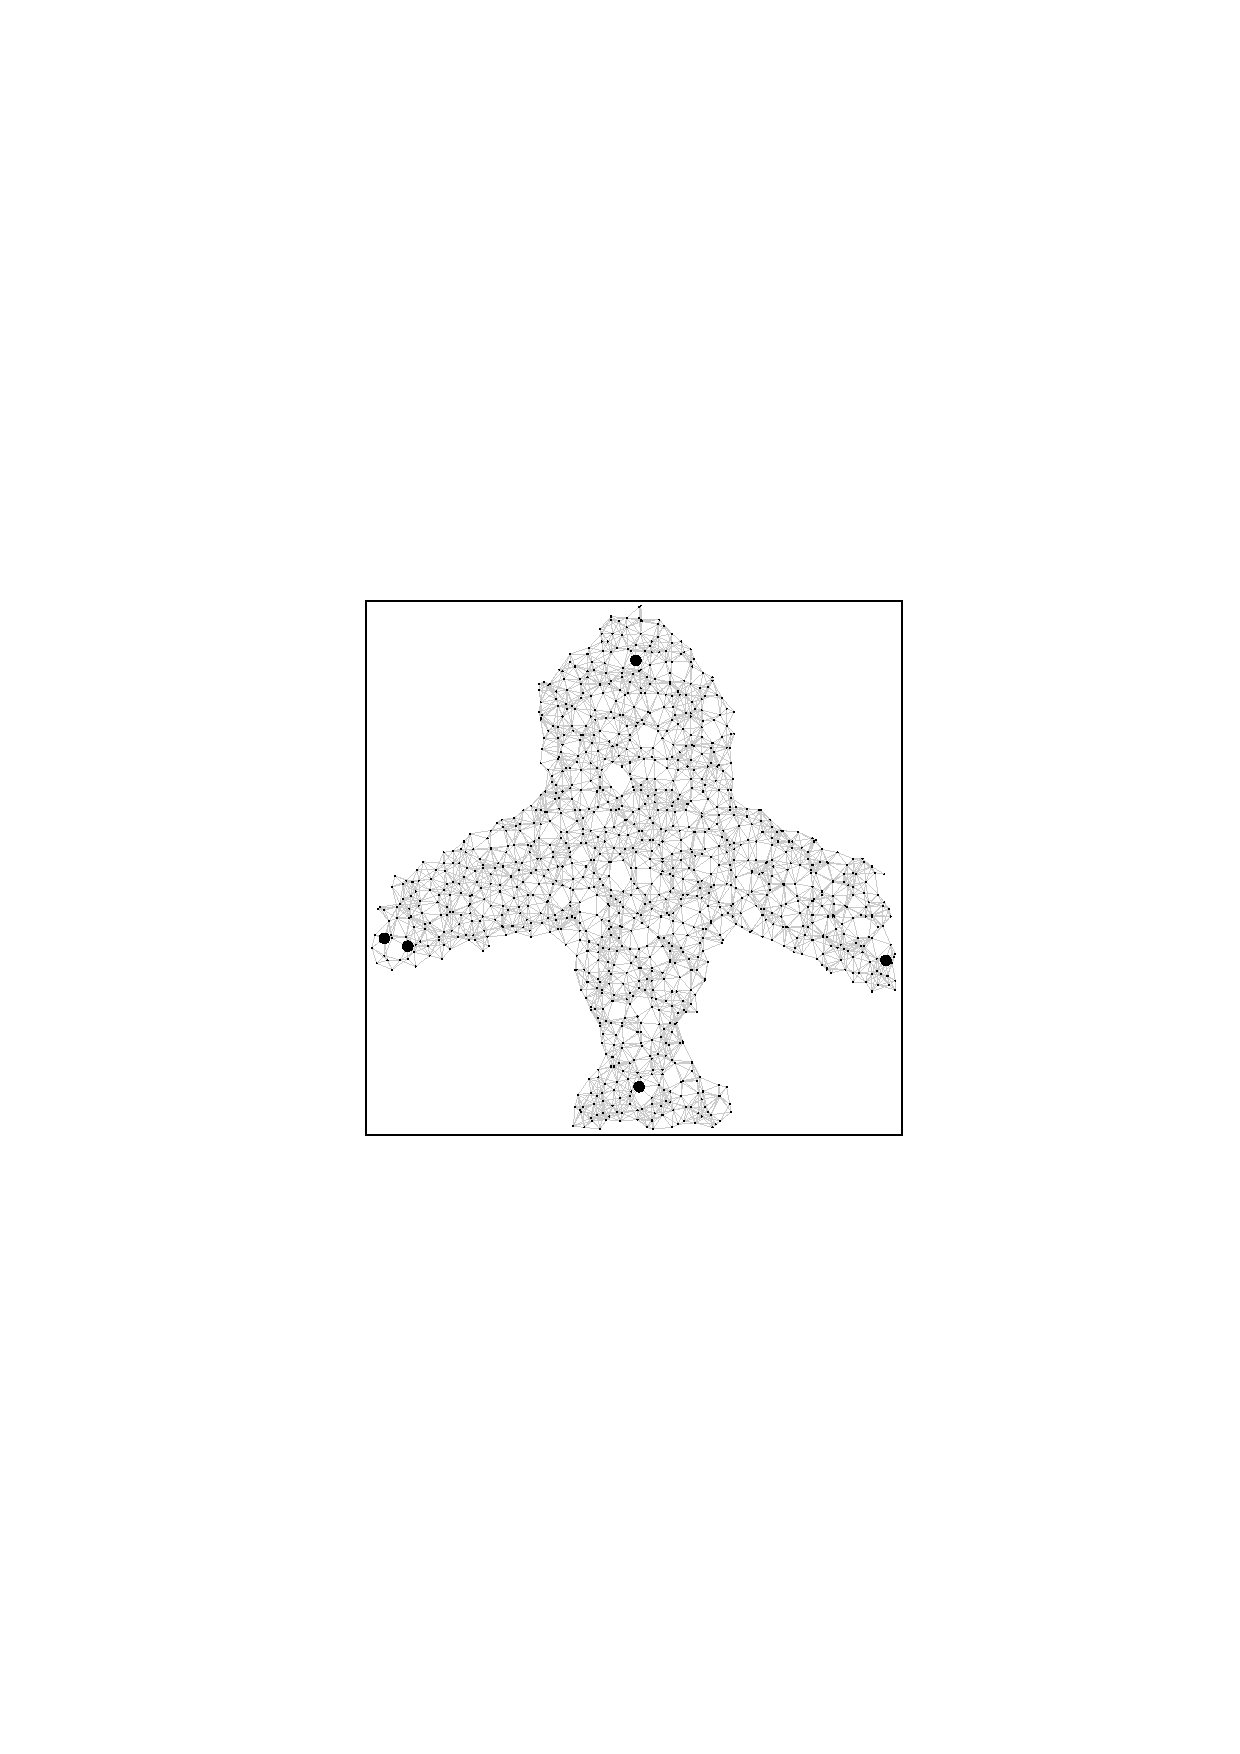
\includegraphics[width=.32\textwidth]{fig305-e}}\hspace{0.25em}%
  \subfloat[]{
    \label{fig:305f}
    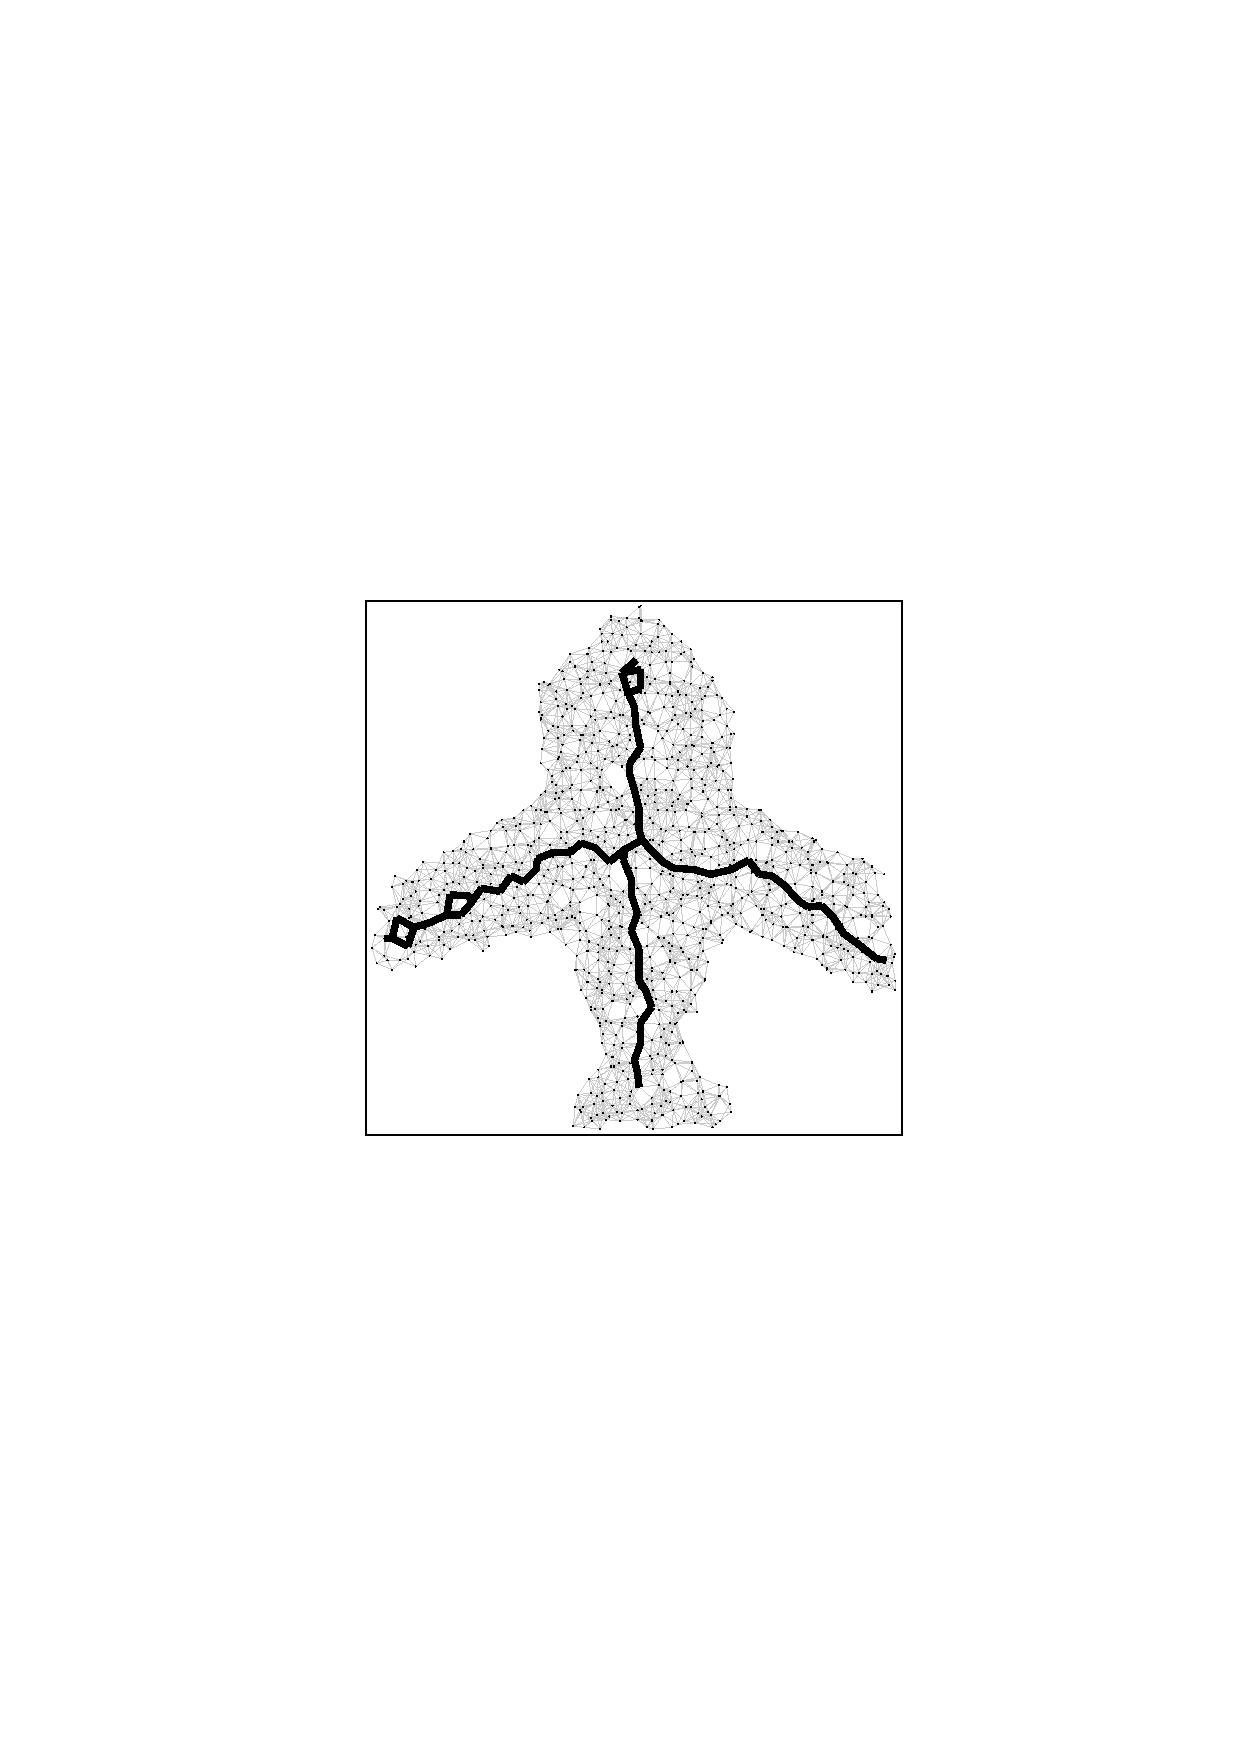
\includegraphics[width=.32\textwidth]{fig305-f}}
\caption{不存在内边界的网络中提取出的骨干带网络及初始骨干}
\label{fig:305}
\end{figure}

下面考虑初始网络中不存在内边界的情况,如图\ref{fig:305a}所示的网络。从该网络中提取出的骨干带网络是开放式的,如图\ref{fig:305b}所示。此时,如果直接利用以上的HPT变换对骨干带网络进行处理,则各分支顶端的节点将可能按照由外而内的顺序逐渐被删除,最终得到图\ref{fig:305c}所示的不完整的原始骨干。该实例中因为部分分支的顶端形成了环结构才没有被全部删除,否则将可能最终仅得到位于网络中心的唯一节点。为了克服这一问题,我们引入了骨干叶节点的概念。简单来说,骨干叶节点就是位于骨干带网络的分支顶端的节点。在仅利用局部连通性信息的情况下,我们利用如下的方式来定义和识别骨干叶节点。对于图\ref{fig:306a}中的节点$u$,其2跳邻居之间的最短路径大部分不通过其1跳邻居;而对于图\ref{fig:306b}中的节点$v$,其2跳邻居之间的最短路径大部分将通过其1跳邻居。基于以上观察结果,我们对骨干叶节点进行定义,如定义\ref{def:303}所述。
\begin{definition}\label{def:303}
对于骨干带网络$\Gamma_{S(G)}$中的任意一点$v$以及常数$\rho$,分别找出其所有的$\rho+1$跳邻居对之间的一条最短路径。若这些路径中均不包含$v$的$\rho$跳邻居,则$v$为骨干叶节点。
\end{definition}
\begin{figure}[h]
  \centering
  \subfloat[]{
    \label{fig:306a}
    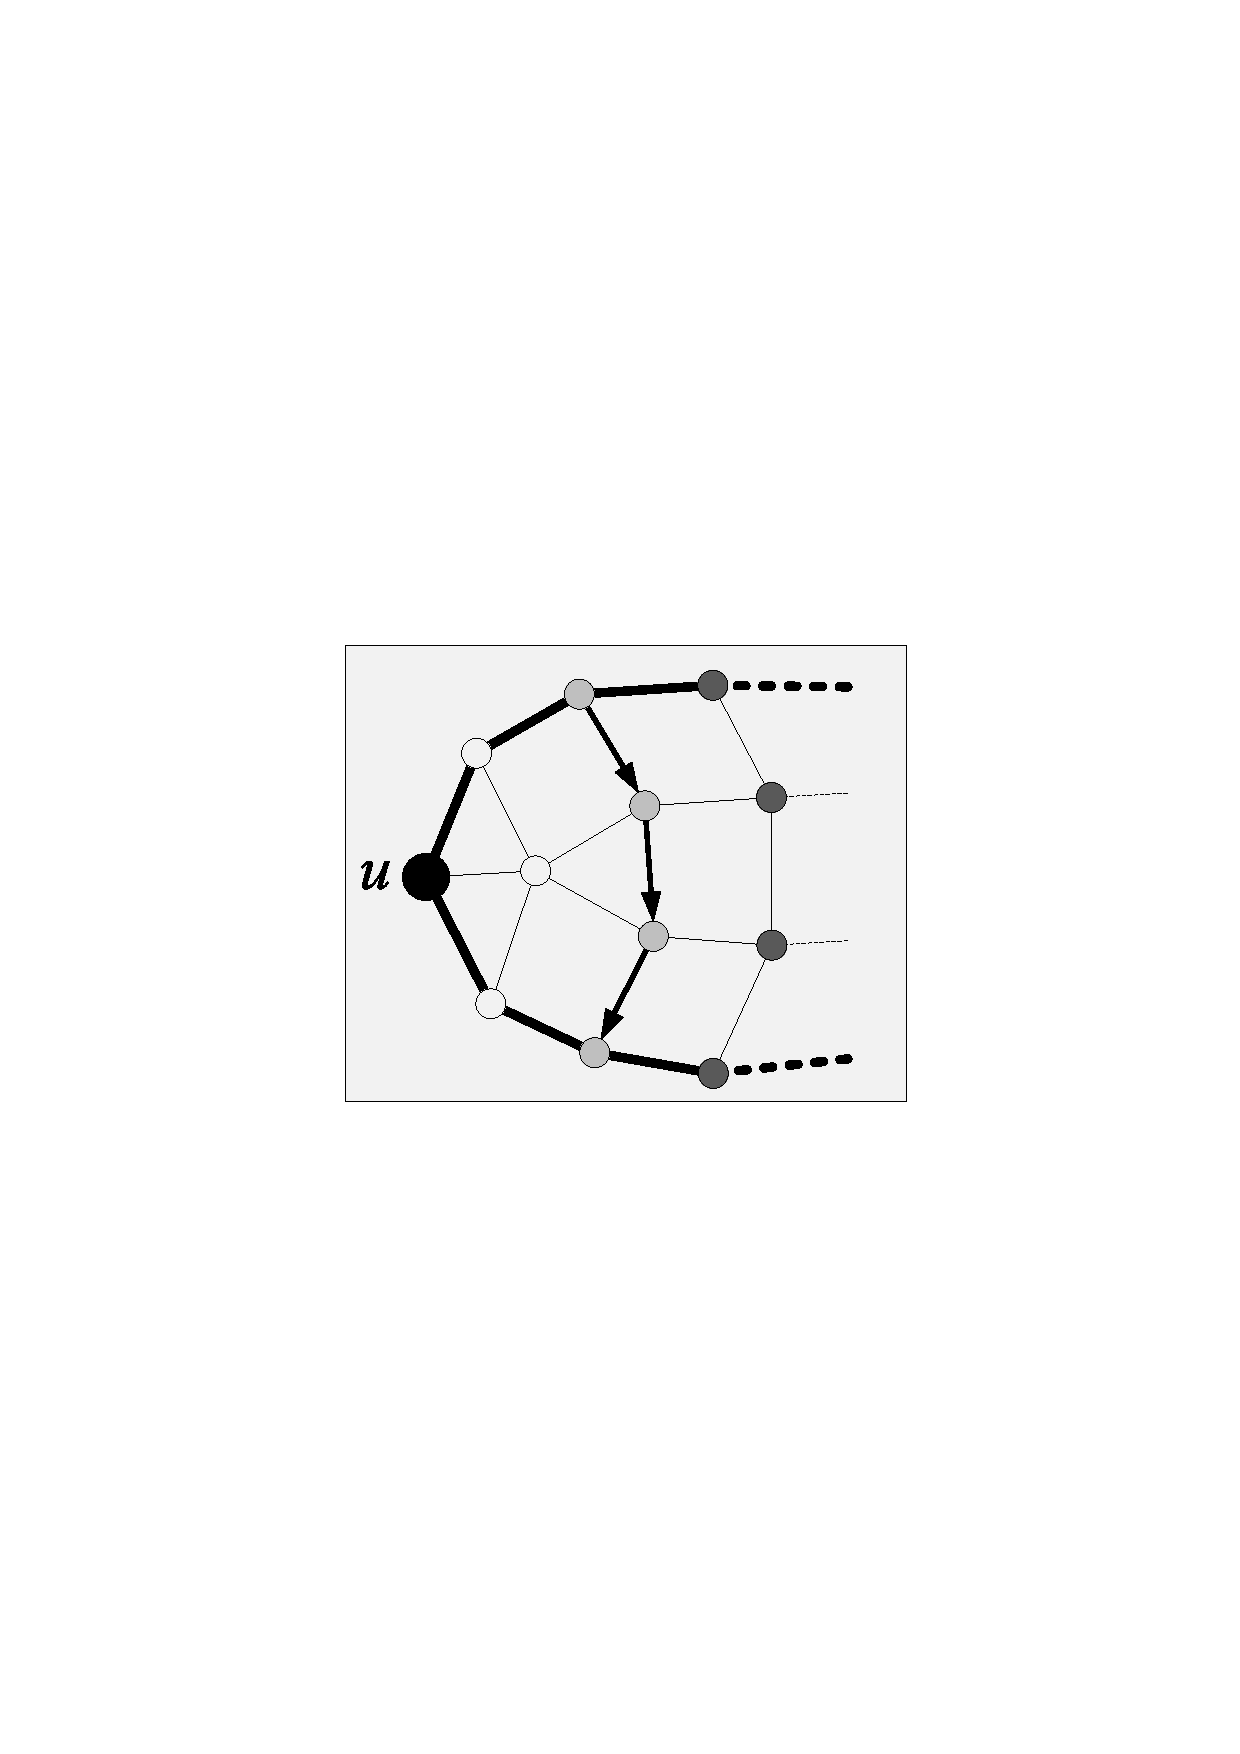
\includegraphics[width=.32\textwidth]{fig306-a}}\hspace{0.5em}%
  \subfloat[]{
    \label{fig:306b}
    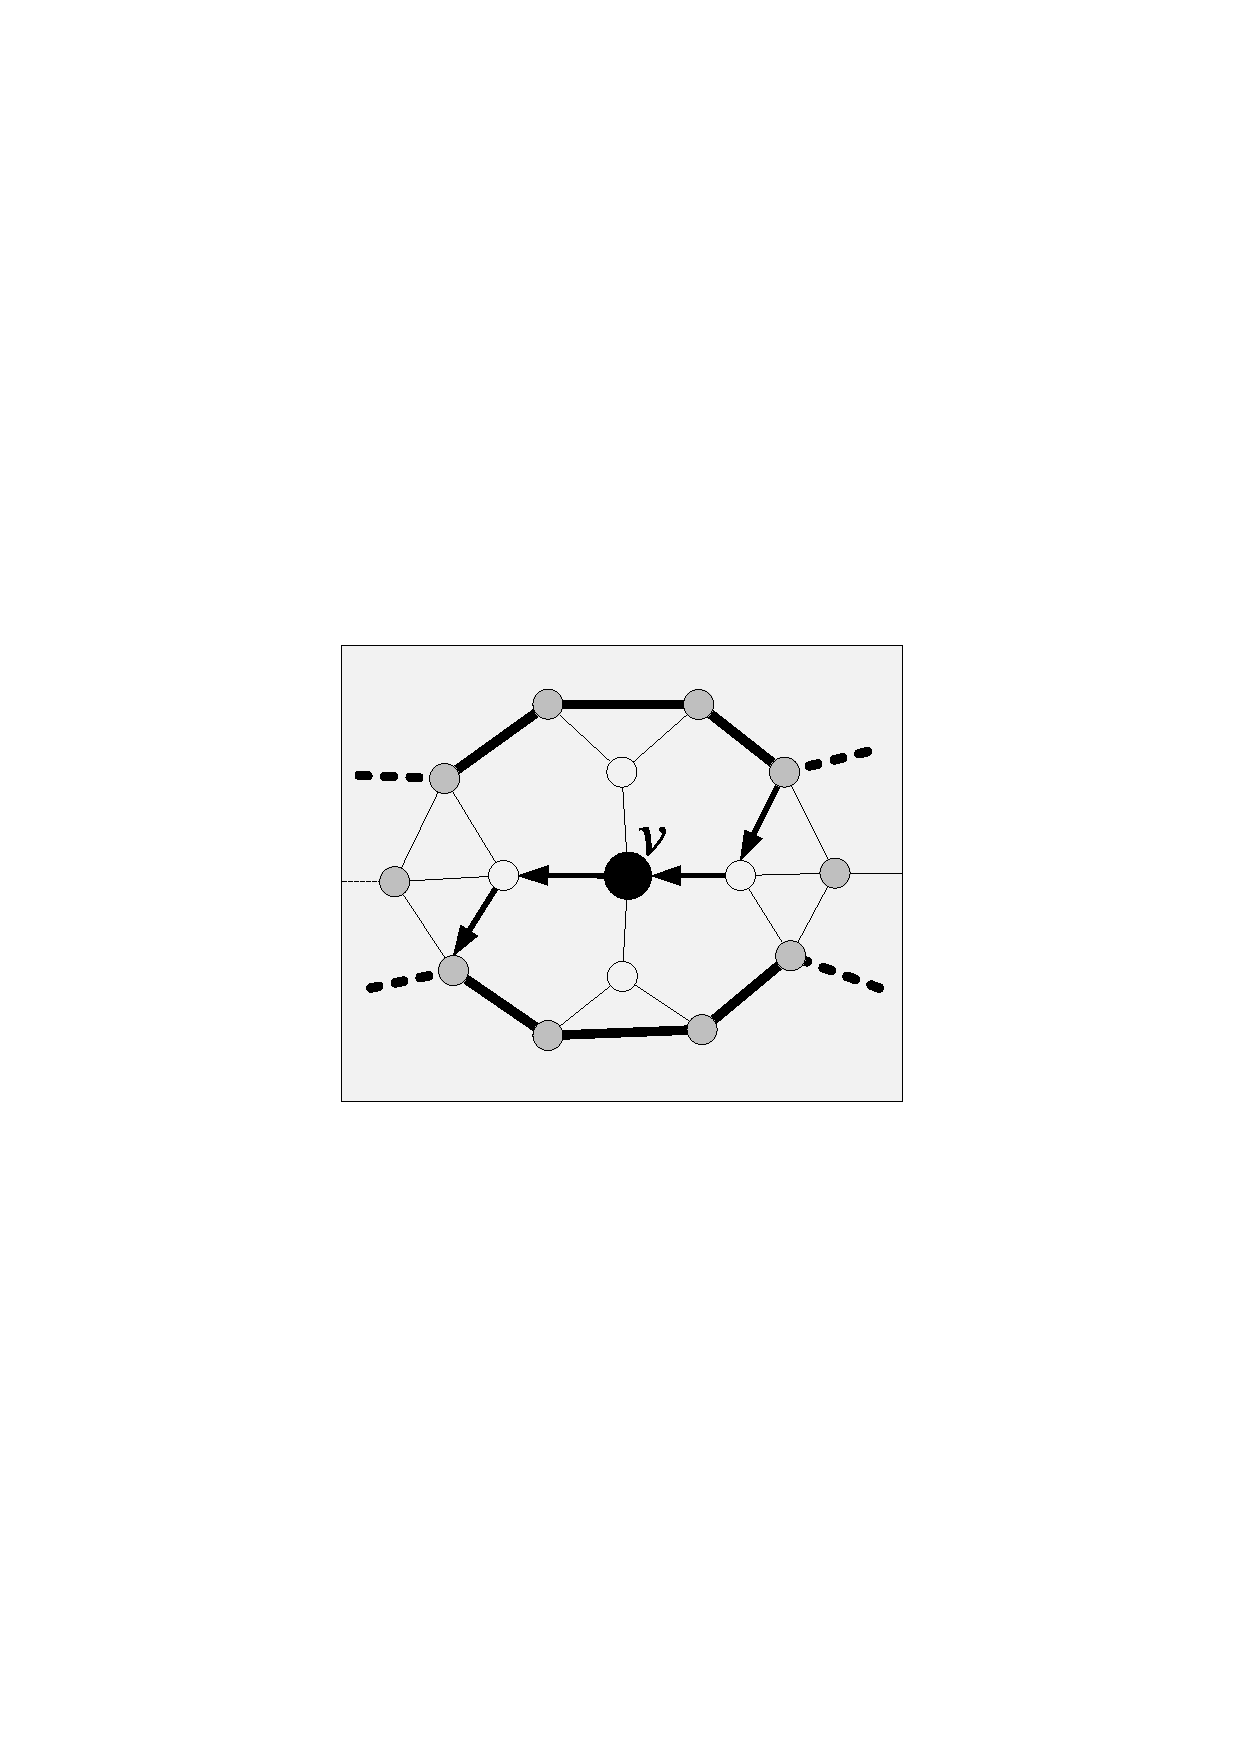
\includegraphics[width=.32\textwidth]{fig306-b}}
\caption{骨干叶节点的定义原则示意图}
\label{fig:306}
\end{figure}

一般情况下,$\rho$仅需设置为较小的值,例如在本章的实验中,取$\rho=1$即可满足大部分的网络实例。按照如上的原则,我们可以得到骨干带网络中的所有骨干叶节点,如图\ref{fig:305d}所示。然后找出这些节点组成的所有连通分支,并在每个连通分支中选择一个邻居数量最少的节点作为最终的骨干叶节点,从而得到如图\ref{fig:305e}所示的骨干叶节点集合,记为$L(\Gamma_{S(G)})$。接下来,我们将所有的骨干叶节点设置为不可删除的,并执行前面所述的HPT变换操作,并得到完整的初始骨干$G_S$,如图\ref{fig:305f}所示。

拓扑骨干提取问题中一个关键的要求就是要得到连通的拓扑骨干,且其形状必须符合实际的整体网络形状。本章提出的算法将骨干节点扩展成具有良好连通性和形状的骨干带网络,然后在骨干带网络中执行HPT变换以得到初始的拓扑骨干。算法能够在一定程度上保证所得到的初始骨干的连通性,如定理\ref{theorem301}所述。
\begin{theorem}
  \label{theorem301}
如果骨干带网络$\Gamma_{S(G)}$是连通的,则利用HPT变换得到的初始骨干$G_S$也是连通的。
\end{theorem}
\begin{proof}
假设骨干带网络$\Gamma_{S(G)}$是连通的,下面分别证明HPT变换的点删除操作和边删除操作均不会破坏骨干带网络的连通性。首先分析点删除操作。按照HPT变换的定义,对于$\Gamma_{S(G)}$中任意的一个点$v$,其可以被删除的第一个条件就是$v$在$\Gamma_{S(G)}$中的1跳邻居子图$\Gamma_{S(G)}(v)$是连通的。由于$\Gamma_{S(G)}(v)$是删除了点$v$之后,由其1跳邻居节点形成的子图,如果$\Gamma_{S(G)}(v)$仍然是连通的,则删除了$v$之后的整个剩余骨干带网络$\Gamma_{S(G)}-v$也一定是连通的。对于边删除操作,由于边$e$可删除的第一个条件也是$e$在$\Gamma_{S(G)}$中的1跳邻居子图$\Gamma_{S(G)}(e)$是连通的,同理可证边删除操作也不会破环骨干带网络的连通性。可见,HPT变换的点删除和边删除均不会破坏骨干带网络的连通性。因此,如果骨干带网络是连通的,则利用HPT变换得到的初始骨干$G_S$也一定是连通的。
\end{proof}
\subsection{剪枝修正}
前一个组件中建立了初始骨干后,接下来对初始骨干执行剪枝修正过程。这是因为在初始骨干中,往往存在一些不需要的较小的局部环结构或者较短的骨干分支,如图\ref{fig:301g}所示。这些较小的局部环结构往往是由于骨干带网络本身存在的一些环,这些环在HPT变换过程中被保留下来;较短的骨干分支一般是由于骨干带网络中一些局部的较小分支中的骨干叶节点被保留下来而形成的。本组件将修剪这些小环和短分支以获得最终的拓扑骨干,仍记为$G_S$,如图\ref{fig:301h}所示。

下面分别介绍小环和短分支的修剪过程。对于小环结构,我们设定一个门限值$\lambda$,长度大于该门限值的环被保留,否则被删除。具体的实现过程如下:原始骨干网络中的每个节点向网络中发送一个范围为$\lambda$的局部的洪泛消息,即该消息仅在$\lambda$跳范围内传播。之后每个骨干节点将得到自身的$\lambda$跳邻居骨干节点信息。然后,节点判断自身的$\lambda$跳骨干子图中是否存在环。若存在环$C$满足$|C|\le\lambda$,则从环$C$中选择一个度数为2的节点,将其从骨干网络中删除。网络中的小环结构按照如上方式被打断,形成了一些较短分支。接下来进行短分支的修剪过程。我们限定一个门限值$\omega$,长度大于该门限值的分支被保留,否则被删除。一般情况下满足$\omega\le\lambda$,因此我们直接利用前面的局部洪泛消息过程中得到的信息,每个节点判断自身是否位于一个长度小于$\omega$的分支上,如果是则将该节点从骨干网络中删除。至此,我们就完成了剪枝修正过程。剪枝修正过程仅删除了局部的小环和较短的分支结构,因此并不会破坏剩余的骨干网络的连通性,如定理\ref{theorem302}所述。该定理的证明非常简单,这里不再赘述。
\begin{theorem}
  \label{theorem302}
对连通的原始骨干网络进行剪枝修正,得到的最终拓扑骨干网络$G_S$仍然是连通的。
\end{theorem}
\subsection{算法及复杂度分析}

\begin{algorithm}[t]
\caption{拓扑骨干提取算法}
\label{alg:301}
\begin{algorithmic}[1]
\REQUIRE ~~\
网络连通图$G(V,E)$
\ENSURE ~~\
拓扑骨干网络$G_S$
\FOR {任意一个节点$v\in{V}$}
    \STATE 获得$v$的$k$跳邻居子图$G_k(v)$,应用MDS算法;
    \IF {MDS算法结果中$v$对应的虚拟节点为边界节点}
        \STATE 将$v$加入边界节点集合$B(G)$;
    \ENDIF
\ENDFOR
\STATE 从$B(G)$中找出边界节点构成的所有连通组件集合$\mathcal{C}$;
\FOR {任意一个节点$v\in{V}$}
    \IF {$v$有两个以上最近的边界分支 or $v$有局部最大的邻居集合}
        \STATE 将$v$加入骨干节点集合$S(G)$;
    \ENDIF
\ENDFOR
\STATE 找出骨干节点构成的连通组件集合$\mathcal{S}$;
\STATE 将骨干节点扩展成唯一的连通分支;
\STATE 将骨干节点扩展至1跳邻居得到骨干带网络$\Gamma_{S(G)}$;
\STATE 找出骨干带网络中的骨干叶节点集合$L(\Gamma_{S(G)})$;
\STATE 保留骨干叶节点,对$\Gamma_{S(G)}$执行HPT变换操作,得到初始骨干图$S_G$;
\FOR {任意一个节点$s\in{S_G}$}
    \STATE 获得$s$的$\lambda$跳邻居子图$S_G^{\lambda}(w)$;
    \IF {$S_G^{\lambda}(w)$中包含环}
        \STATE 选择环中一个节点度为2的节点并从$S(G)$中删除;
    \ENDIF
\ENDFOR
\FOR {任意一个节点$s\in{S_G}$}
    \STATE 获得$s$的$\omega$跳邻居子图$S_G^{\omega}(w)$;
    \IF {$S_G^{\lambda}(w)$中包含一个长度小于$\omega$的分支}
        \STATE 将该分支中的所有节点从$S(G)$中删除;
    \ENDIF
\ENDFOR
\STATE 输出最终的骨干节点集合$S(G)$以及骨干网络$S_G$;
\end{algorithmic}
\end{algorithm}
完整的拓扑骨干提取算法如算法\ref{alg:301}所示。下面分析算法的时间和消息复杂度,如定理\ref{theorem303}所示。
\begin{theorem}
  \label{theorem303}
拓扑骨干提取算法整体的时间复杂度和消息复杂度均为$\mathcal{O}(\sqrt{n})$。
\end{theorem}
\begin{proof}首先分析算法的时间复杂度。在第一个组件中,边界识别过程中执行MDS算法的时间复杂度为邻居子图中节点数量$m$的多项式时间$\mathcal{O}(m^3)$\upcite{mds_complexity}。$m$值的上限为$\Delta^{k+1}-1)/(\Delta-1)$,其中$\Delta$表示节点度的最大值,$k$表示邻居子图的范围,因此该时间复杂度为$\mathcal{O}(\Delta^{3k})$。因为$k$一般取较小的常数,当最大节点度$\Delta$存在常数上限时,该组件的时间复杂度降低为常数复杂度$\mathcal{O}(1)$。在第二个组件中,每个节点通过局部的洪泛消息判断是否存在两个以上的最近边界节点。在分布式执行的情况下,该过程的时间复杂度为常数复杂度$\mathcal{O}(1)$。但是在最差情况下,假设节点距离边界非常远,如在一个均匀分布的正方形网络区域中,节点到边界的距离的上限为$\sqrt{n}$,其中$n$为网络的节点数量,则此时的时间复杂度为$\mathcal{O}(\sqrt{n})$。但实际上这种情况出现的概率极低。在第三个组件中,算法仅涉及到一些局部的邻居信息收集以及简单的连通性判断操作,因此该部分的时间复杂度为常数复杂度$\mathcal{O}(1)$。在第四个组件中,算法同样仅涉及到一些局部的信息收集和简单的分支长度判断操作,因此在最大节点度存在常数上限时,该部分的时间复杂度仍为常数复杂度$\mathcal{O}(1)$。

然后分析算法的消息复杂度。在第一个组件中,每个节点需要收集局部的邻居信息。因为邻居范围$k$一般取较小的常数,所以当网络的最大节点度$\Delta$存在常数上限时,该部分的消息复杂度为常数复杂度$\mathcal{O}(1)$。在第二个组件中,每个边界节点向网络中发送局部的洪泛消息。假设边界节点的数量为$\sqrt{n}$,则这部分的消息复杂度为$\mathcal{O}(\sqrt{n})$。在第三和第四个组件中,算法均是仅涉及到一些局部的邻居信息收集操作,因此在最大节点度存在常数上限时,该部分的消息复杂度为常数复杂度$\mathcal{O}(1)$。
\end{proof}
\section{实验评估}
本节通过大量的仿真实验对提出的拓扑骨干提取算法的性能进行评估,并对一些可能影响到算法性能的参数进行分析。
\begin{figure}[h]
  \centering
  \subfloat[1572,10.09]{
    \label{fig:307a}
    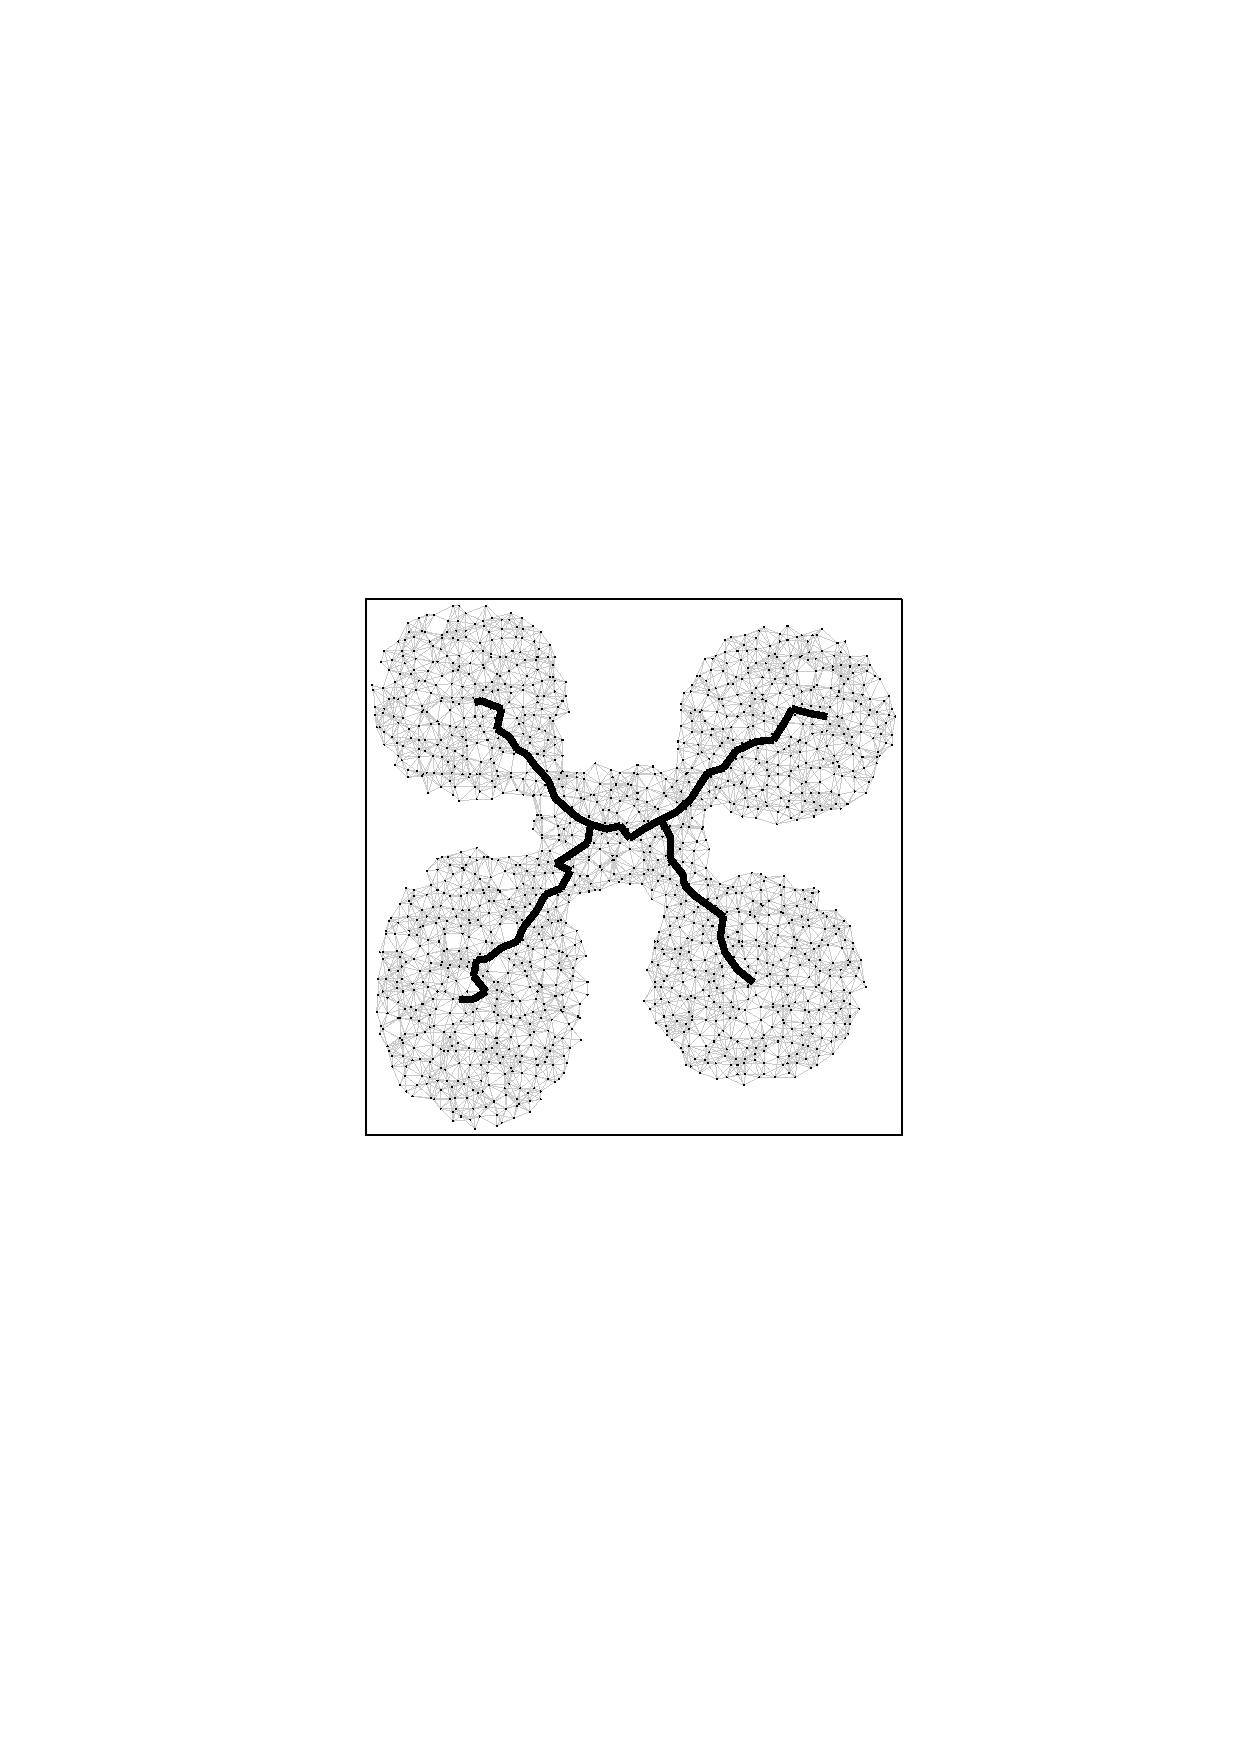
\includegraphics[width=.29\textwidth]{fig307-a}}\hspace{0.25em}%
  \subfloat[3044,10.88]{
    \label{fig:307b}
    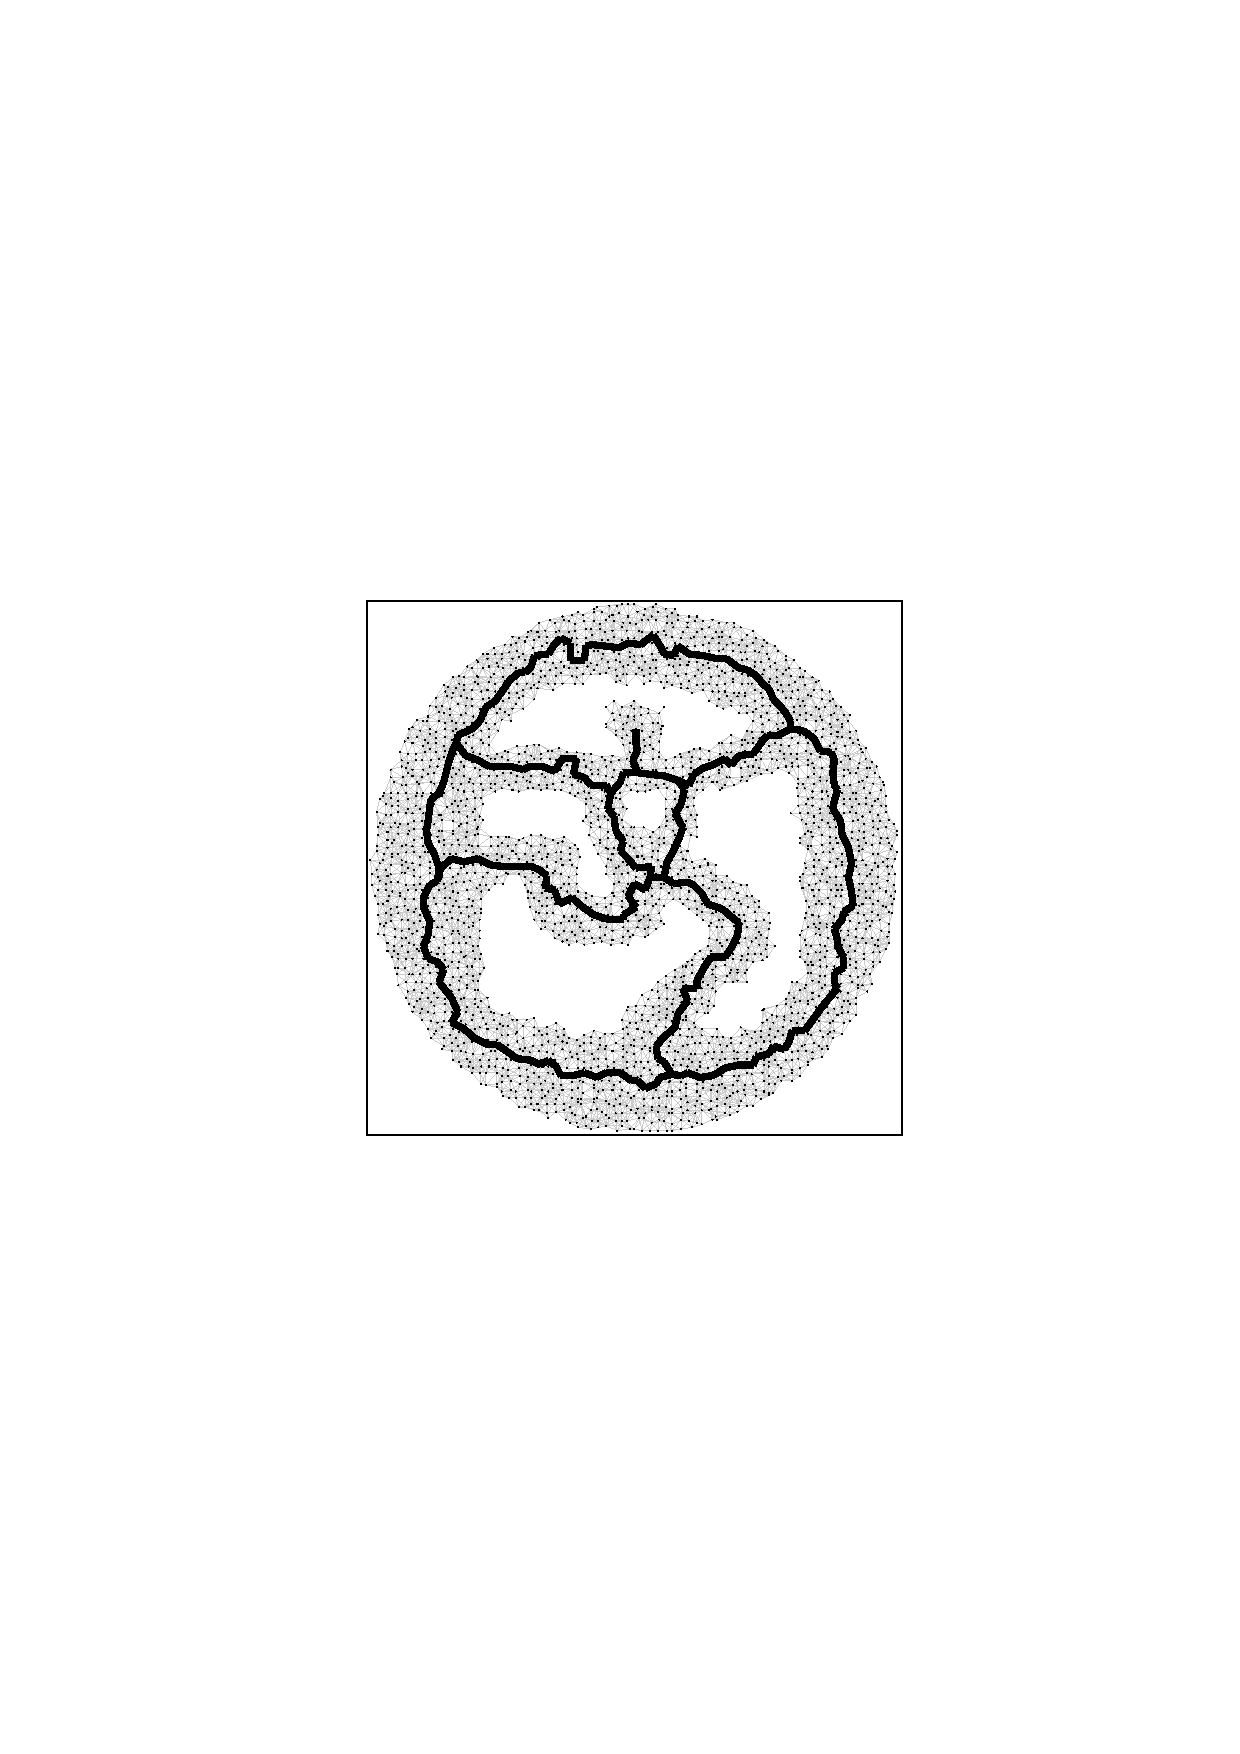
\includegraphics[width=.29\textwidth]{fig307-b}}\hspace{0.25em}%
  \subfloat[1288,11.16]{
    \label{fig:307c}
    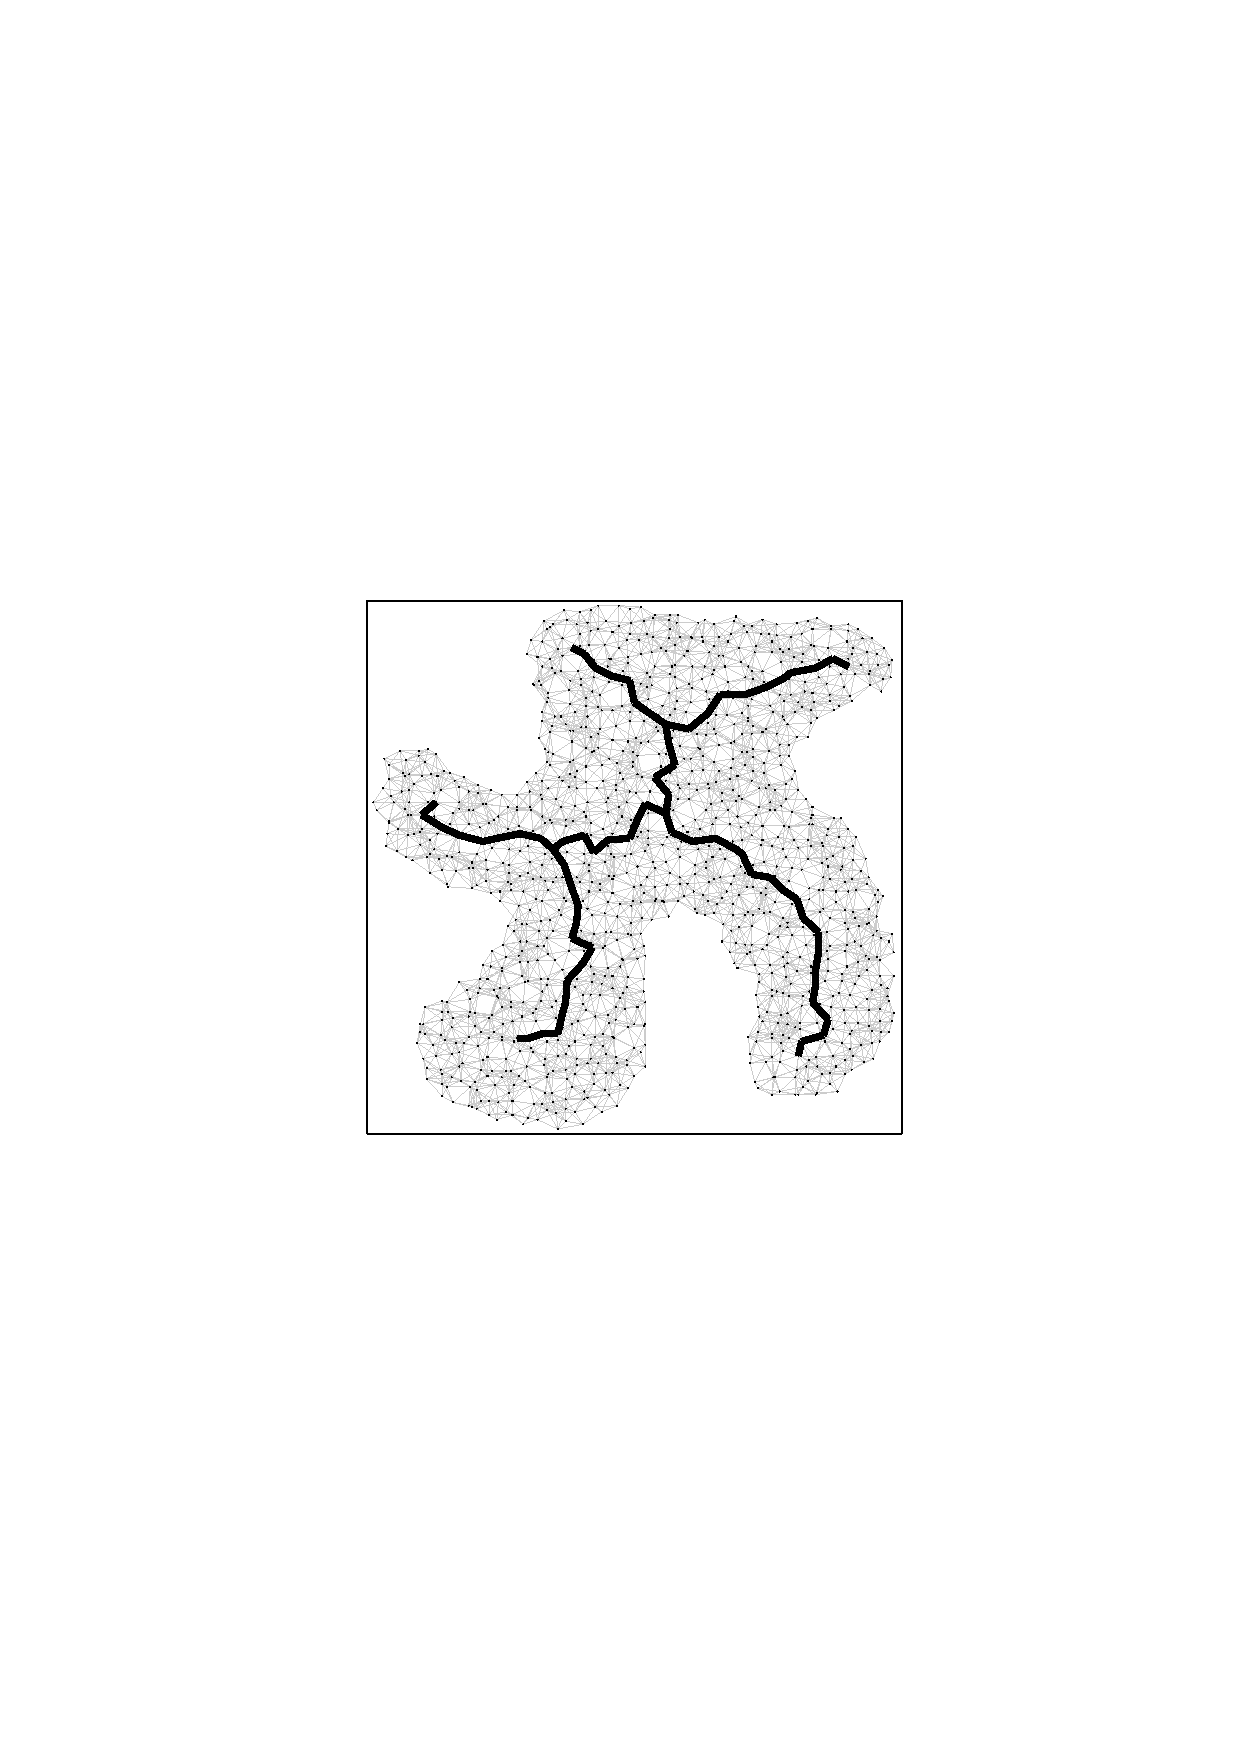
\includegraphics[width=.29\textwidth]{fig307-c}}\hspace{0.25em}%
  \subfloat[1953,10.96]{
    \label{fig:307d}
    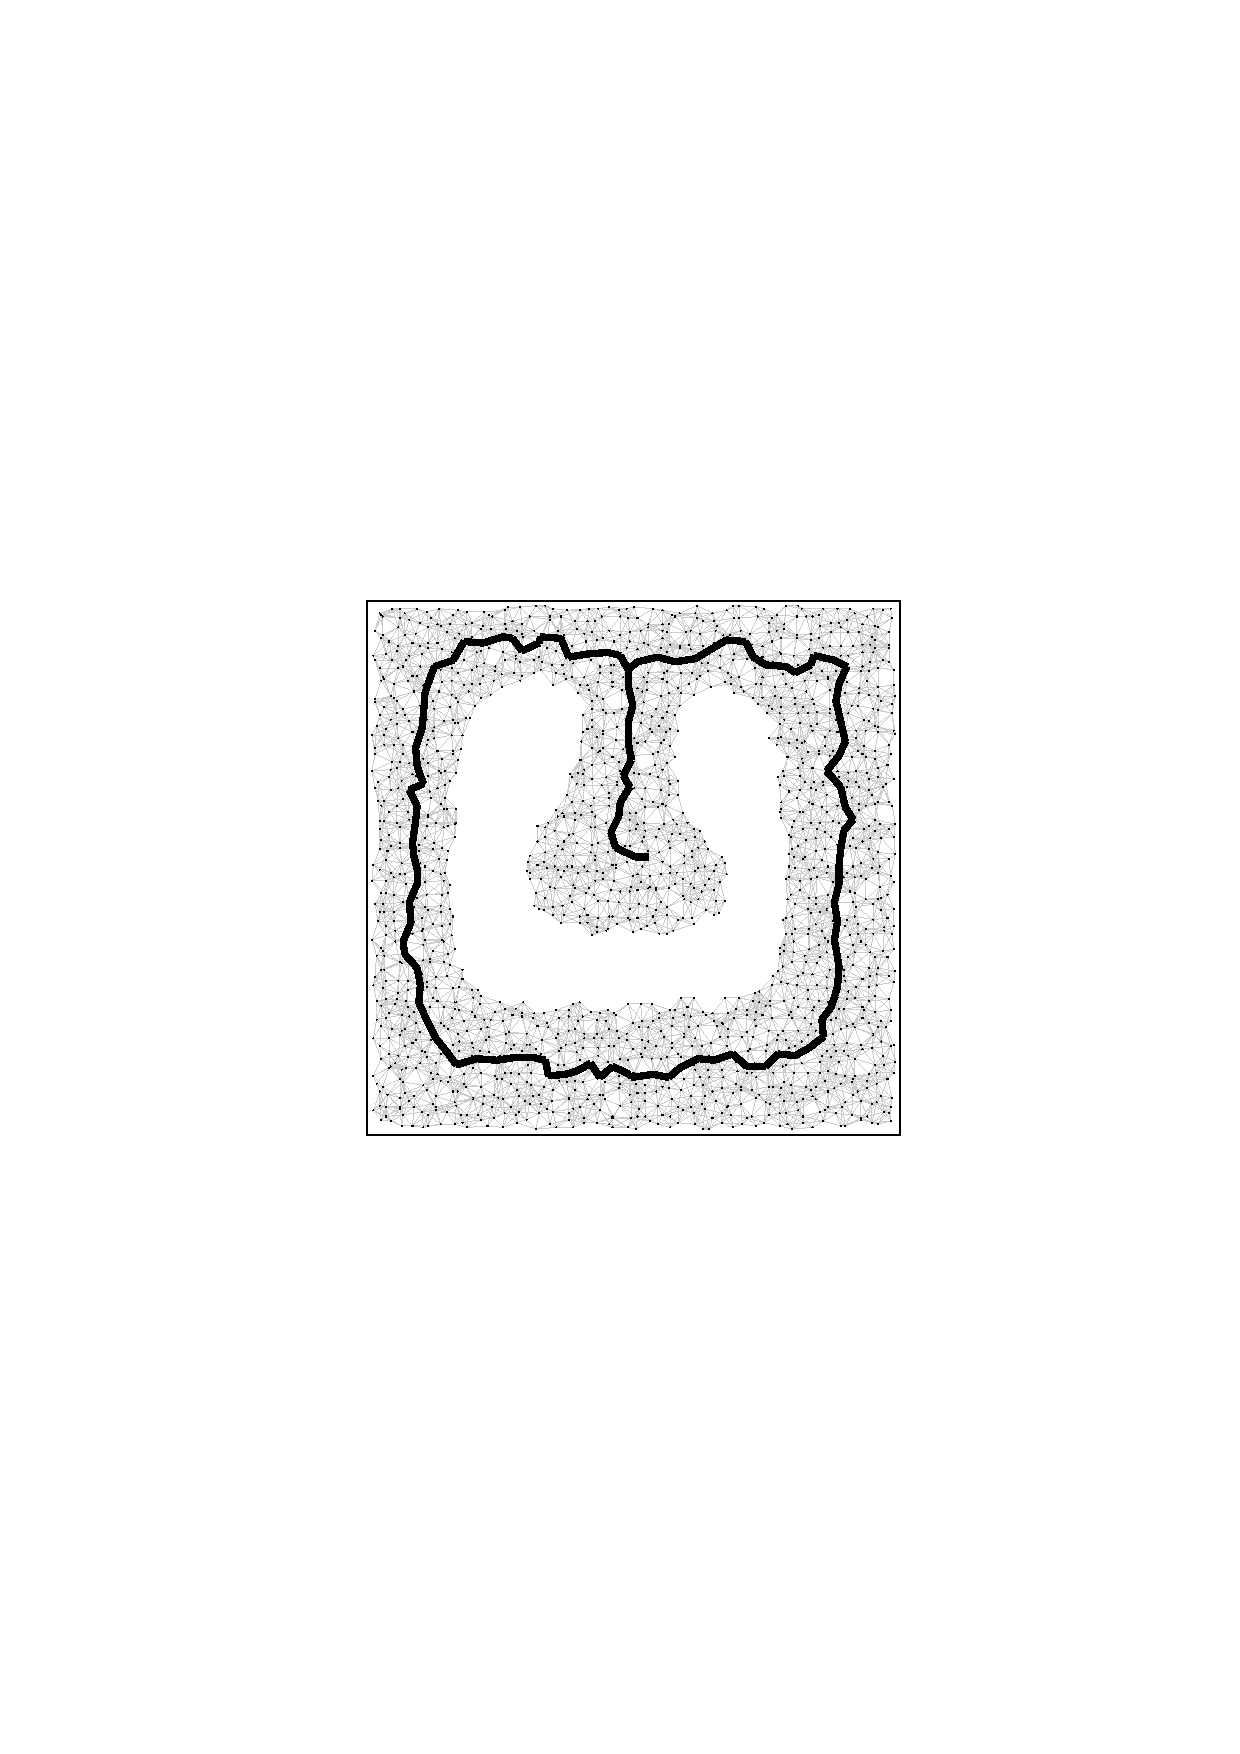
\includegraphics[width=.29\textwidth]{fig307-d}}\hspace{0.25em}%
  \subfloat[2095,11.02]{
    \label{fig:307e}
    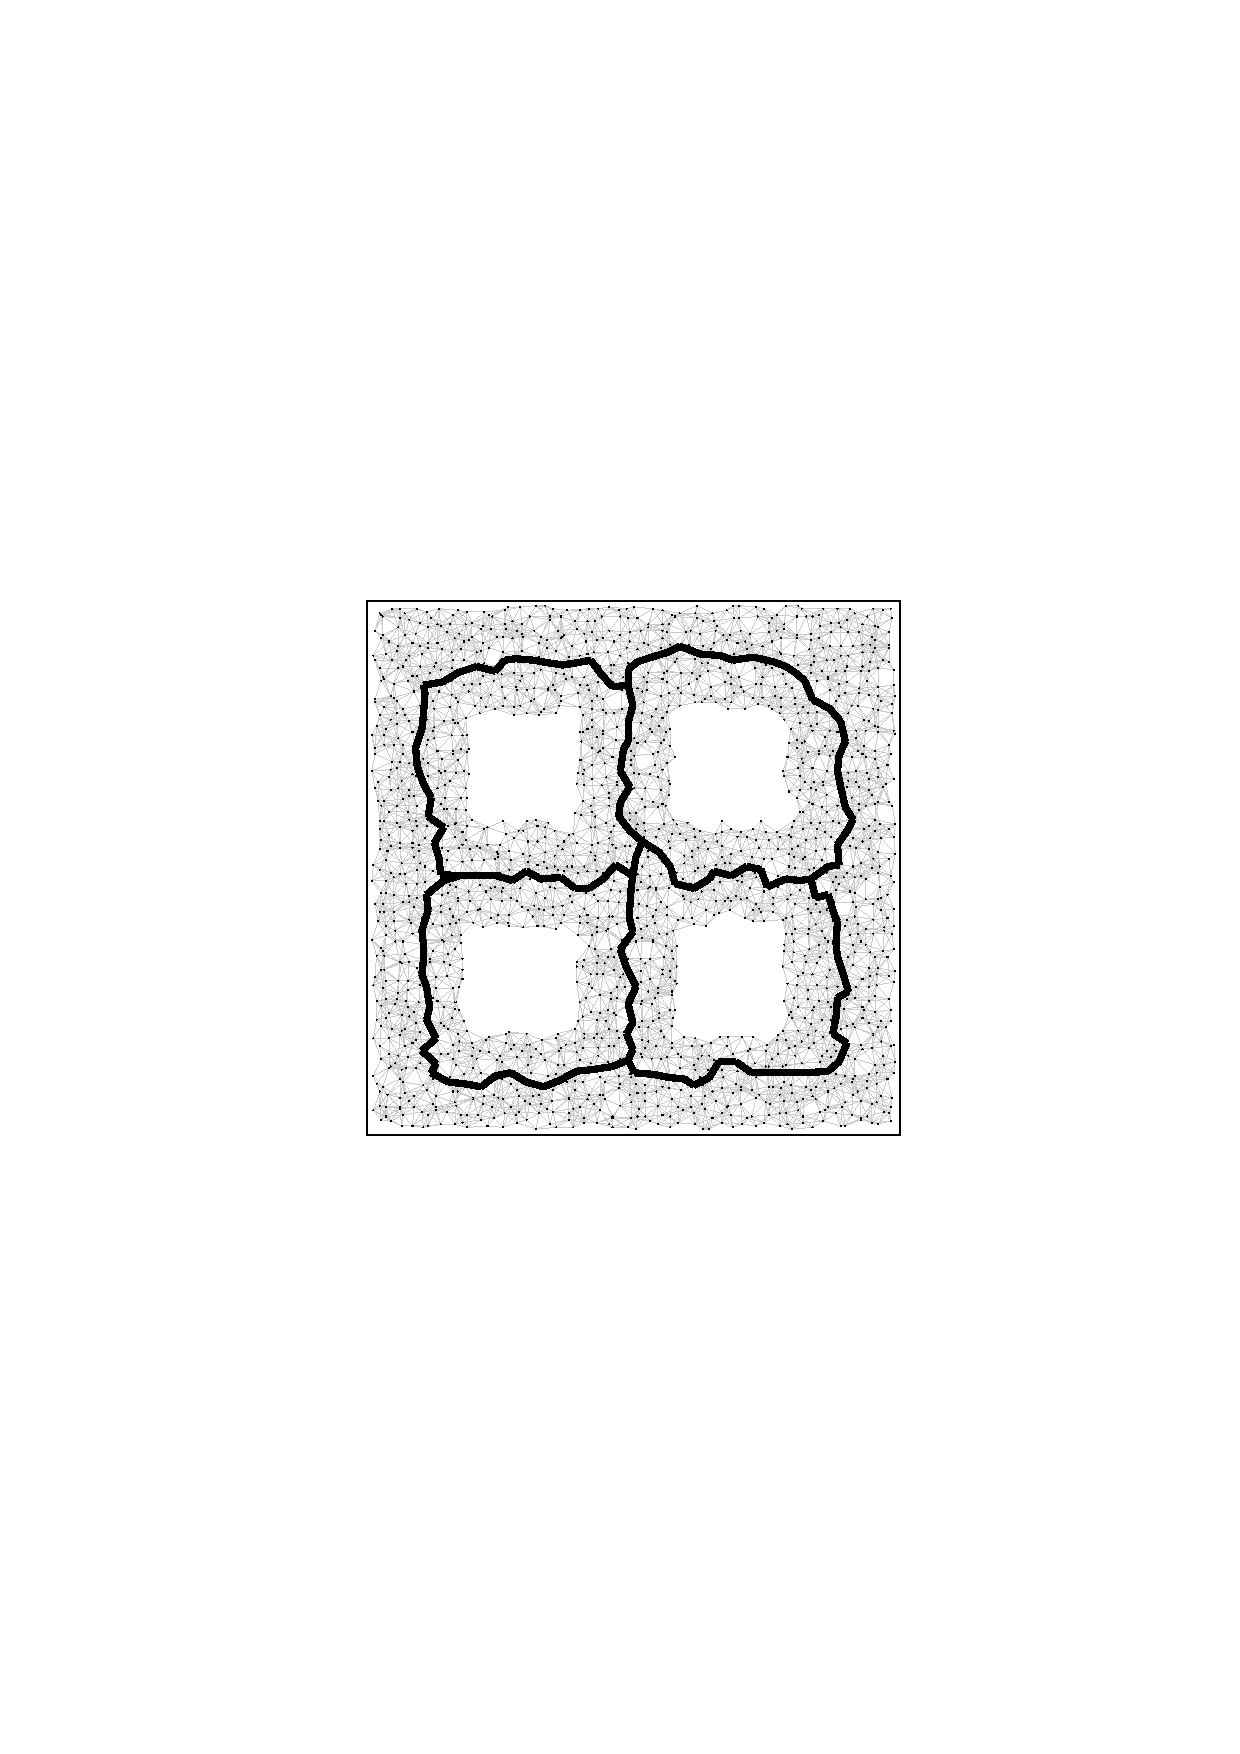
\includegraphics[width=.29\textwidth]{fig307-e}}\hspace{0.25em}%
  \subfloat[1161,11.07]{
    \label{fig:307f}
    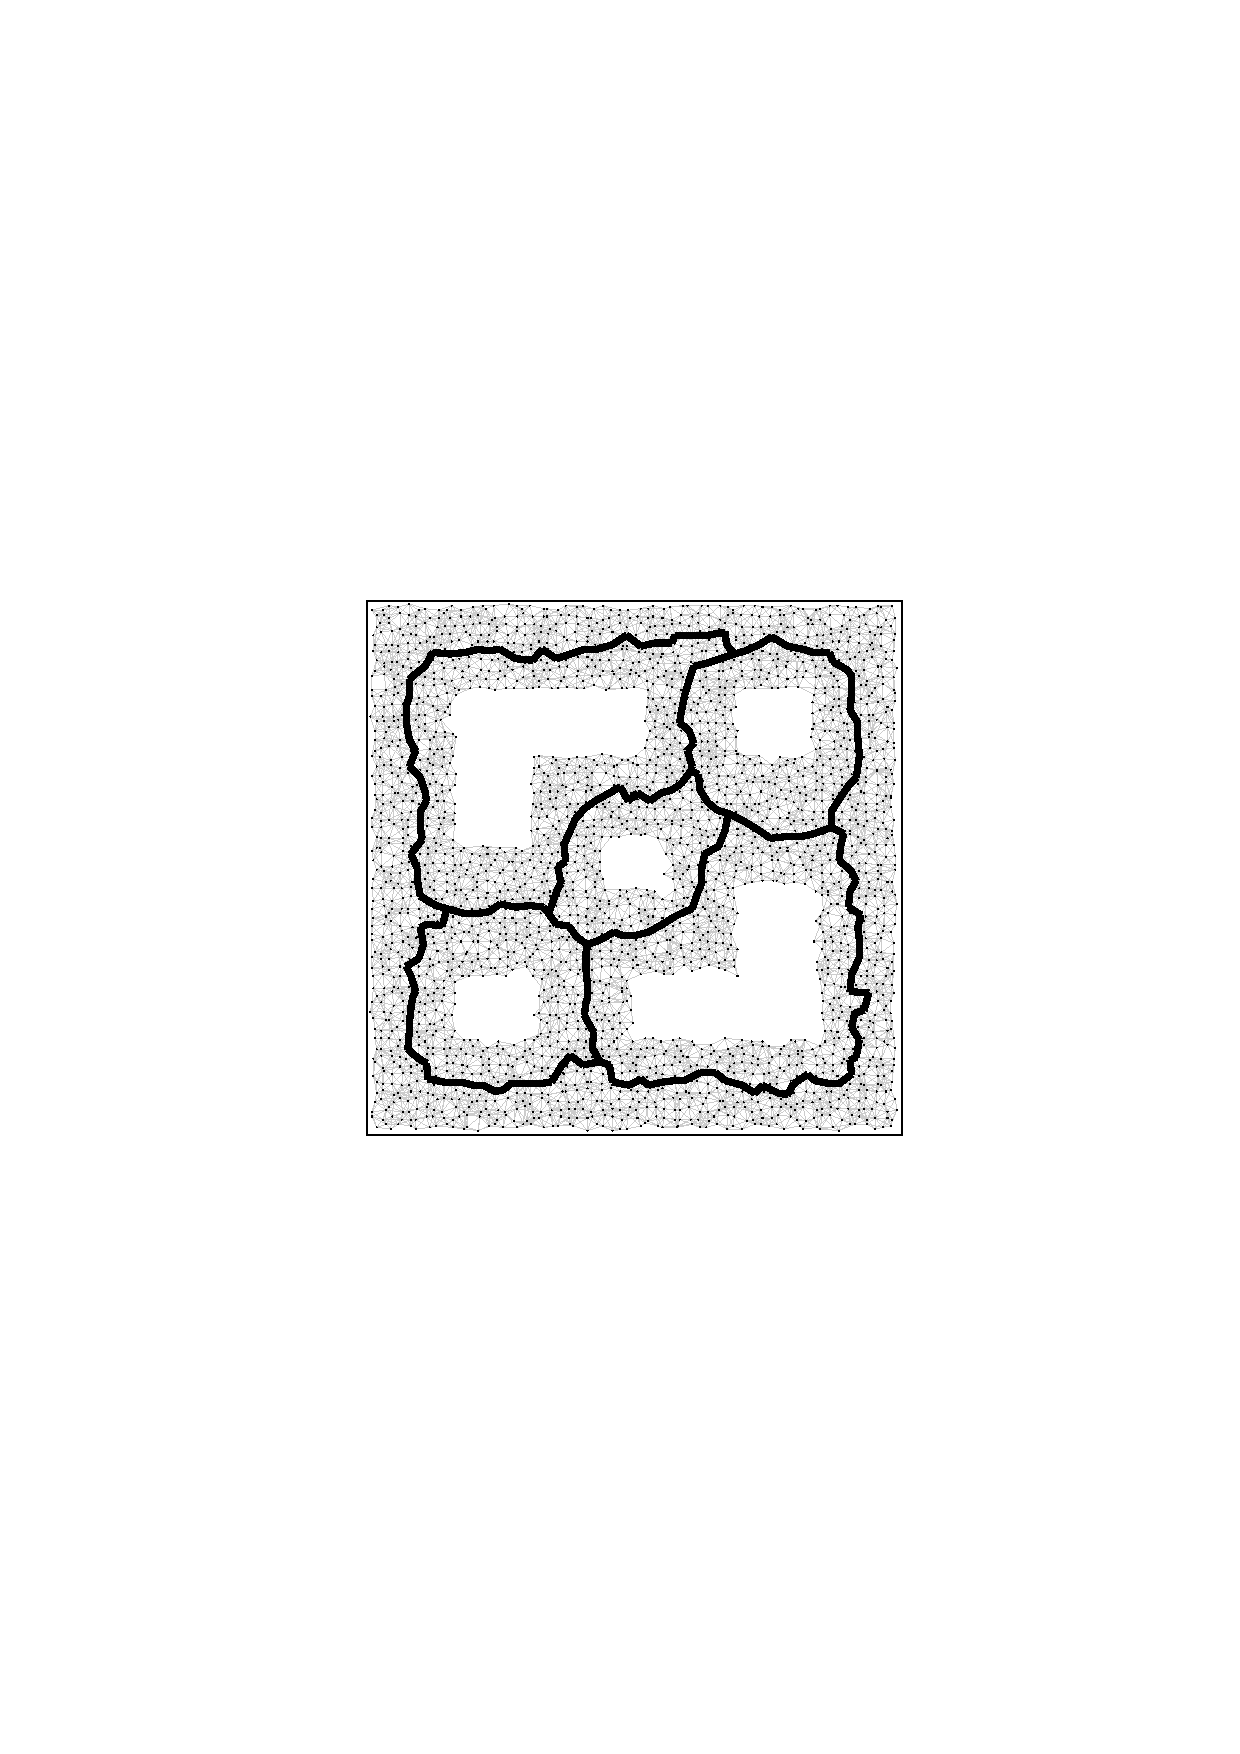
\includegraphics[width=.29\textwidth]{fig307-f}}\hspace{0.25em}%
  \subfloat[1246,11.01]{
    \label{fig:307g}
    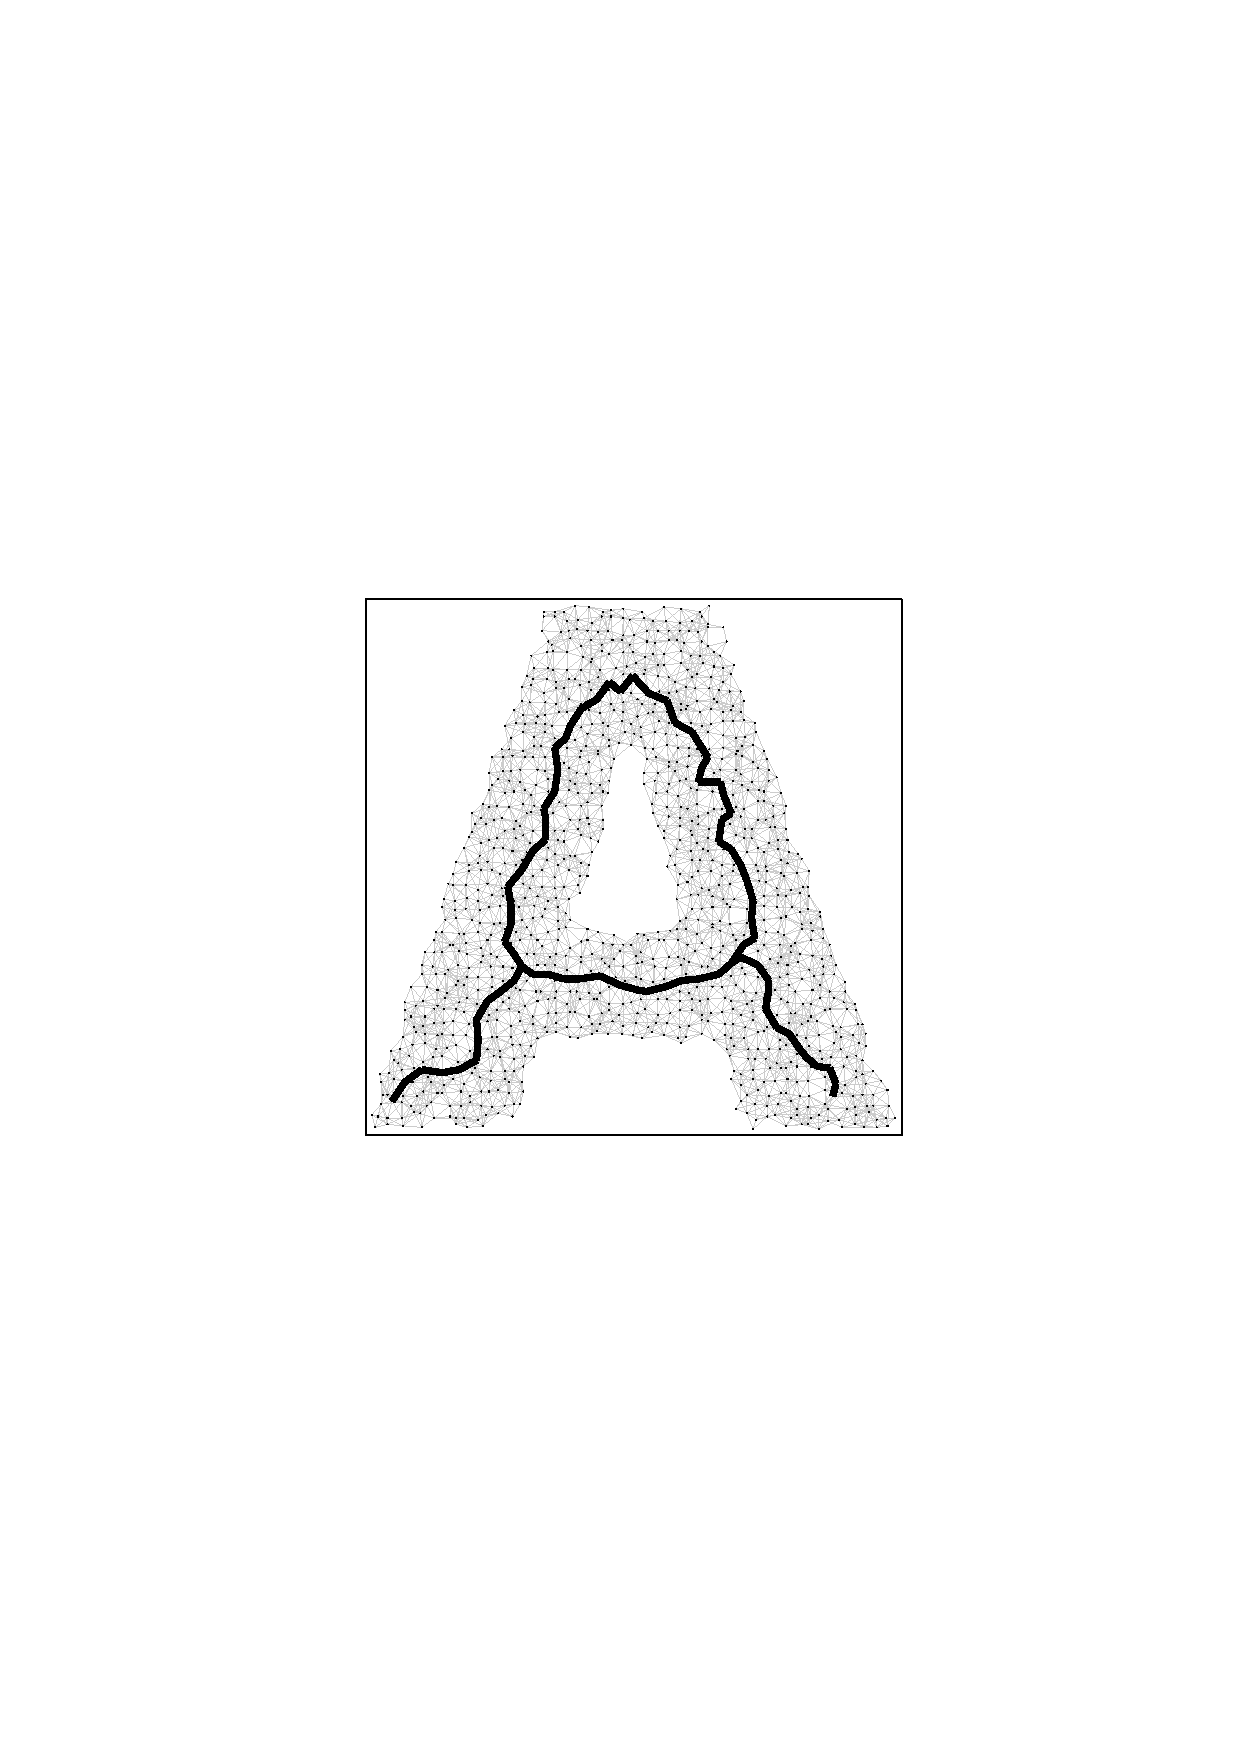
\includegraphics[width=.29\textwidth]{fig307-g}}\hspace{0.25em}%
  \subfloat[2201,11.14]{
    \label{fig:307h}
    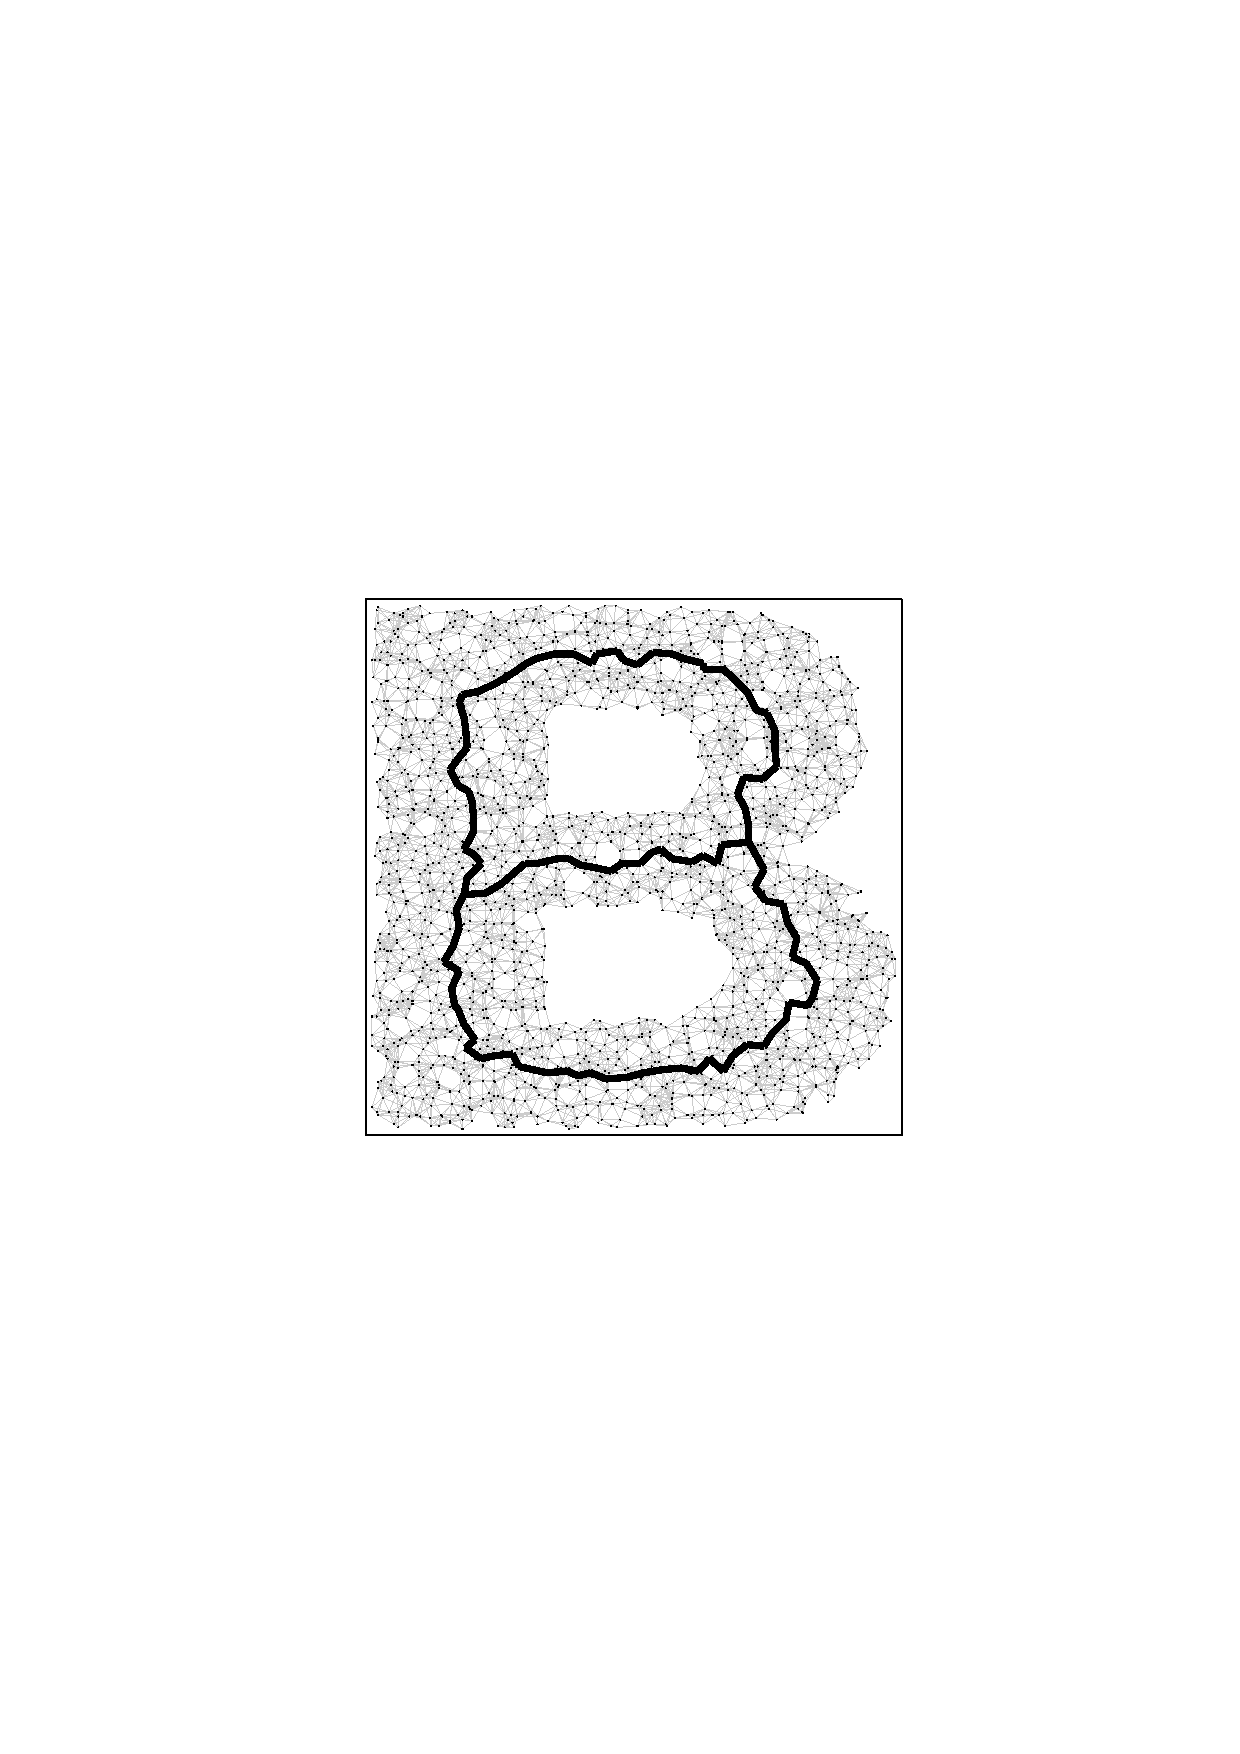
\includegraphics[width=.29\textwidth]{fig307-h}}\hspace{0.25em}%
  \subfloat[1164,11.04]{
     \label{fig:307i}
    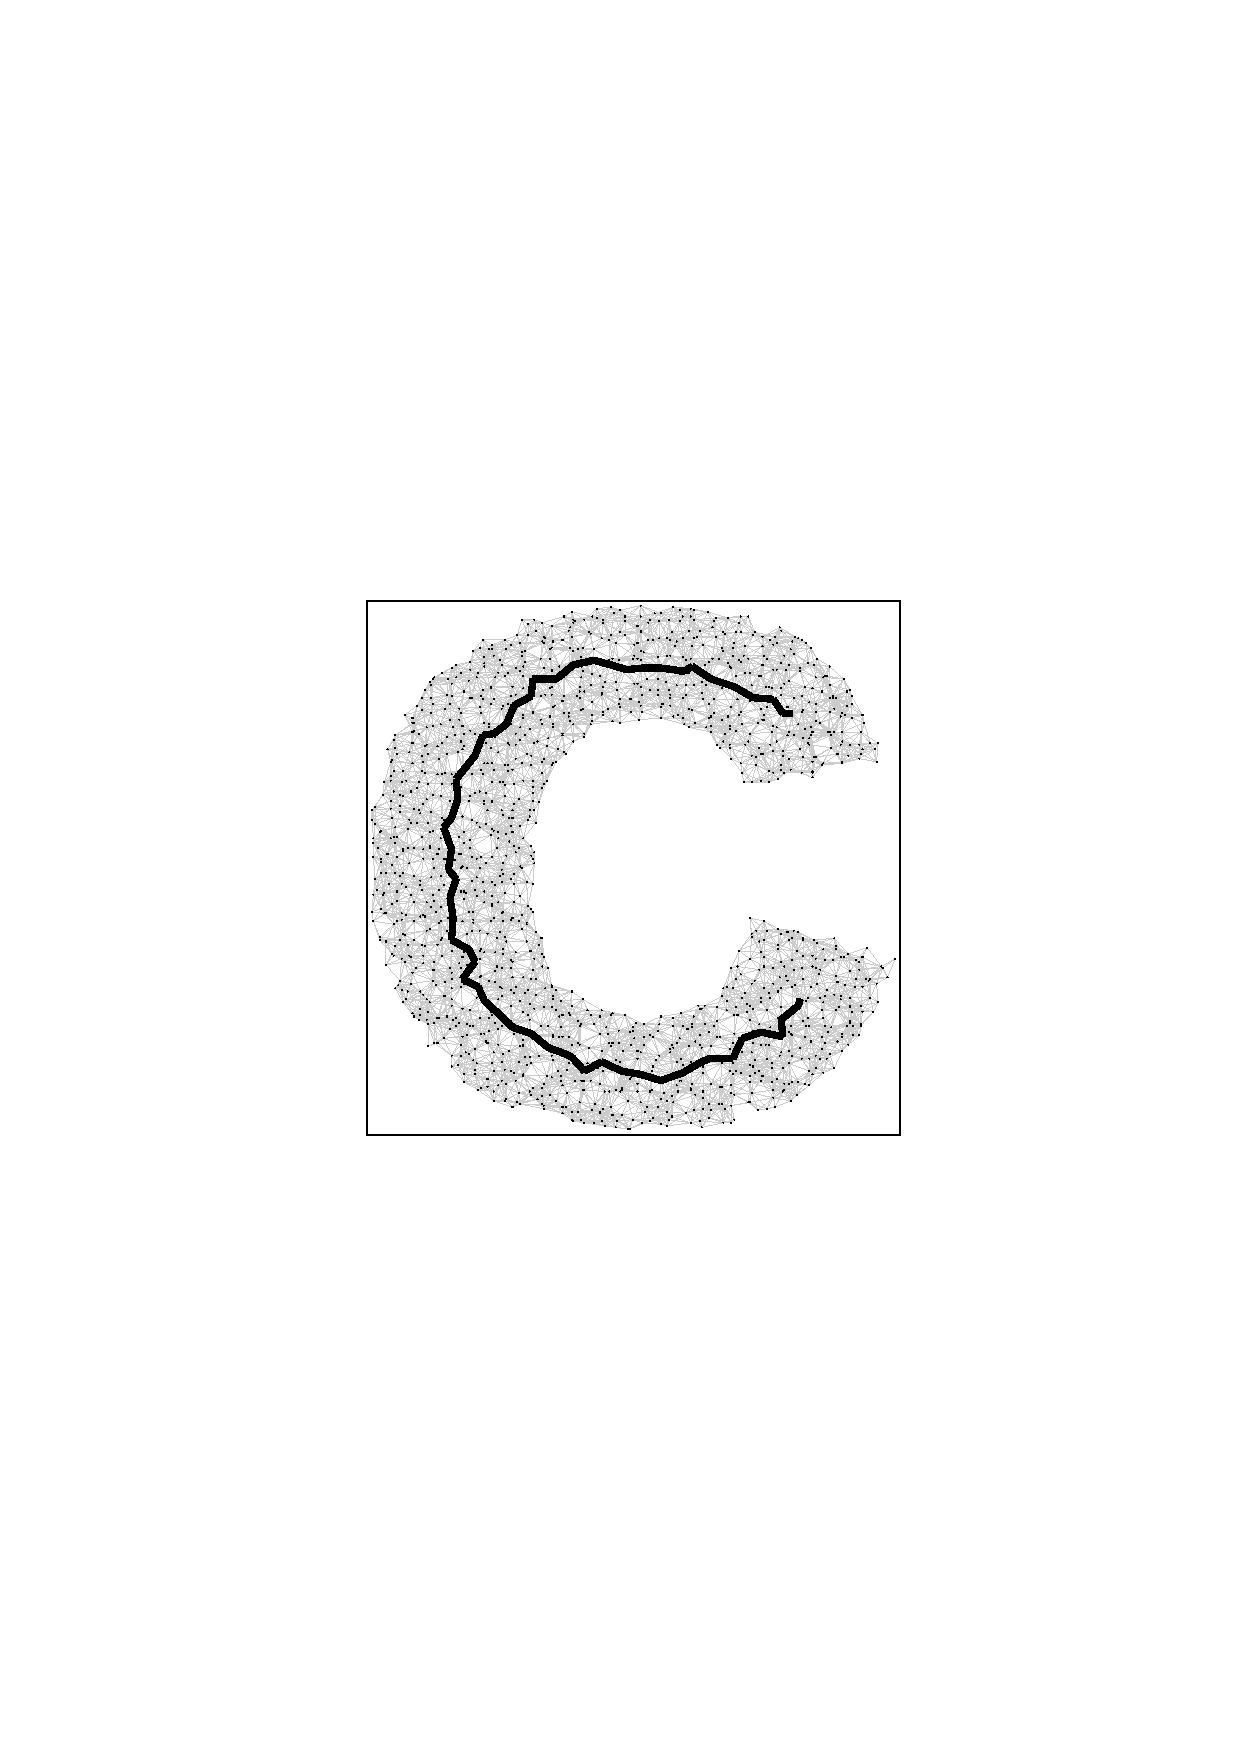
\includegraphics[width=.29\textwidth]{fig307-i}}\hspace{0.25em}%
  \subfloat[1626,11.15]{
    \label{fig:307j}
    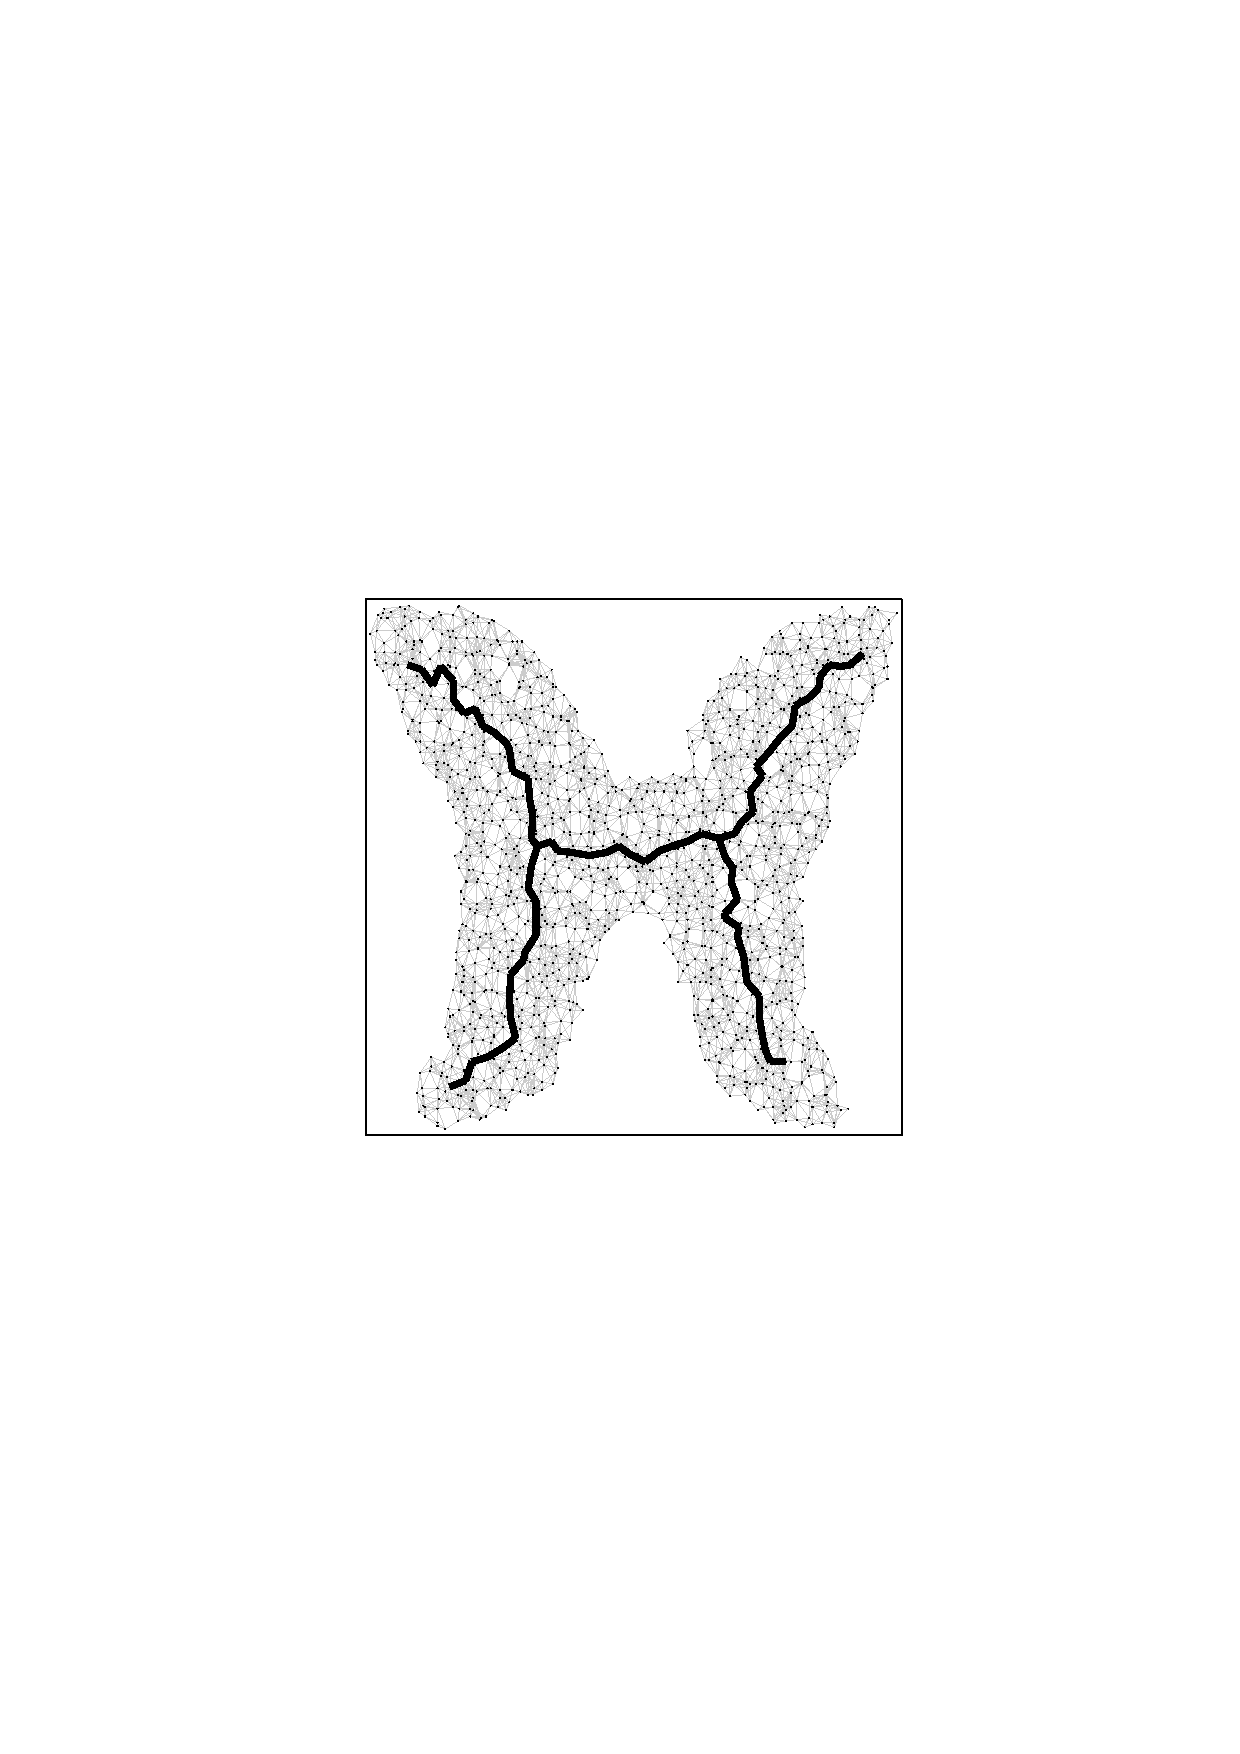
\includegraphics[width=.29\textwidth]{fig307-j}}\hspace{0.25em}%
  \subfloat[2978,11.01]{
    \label{fig:307k}
    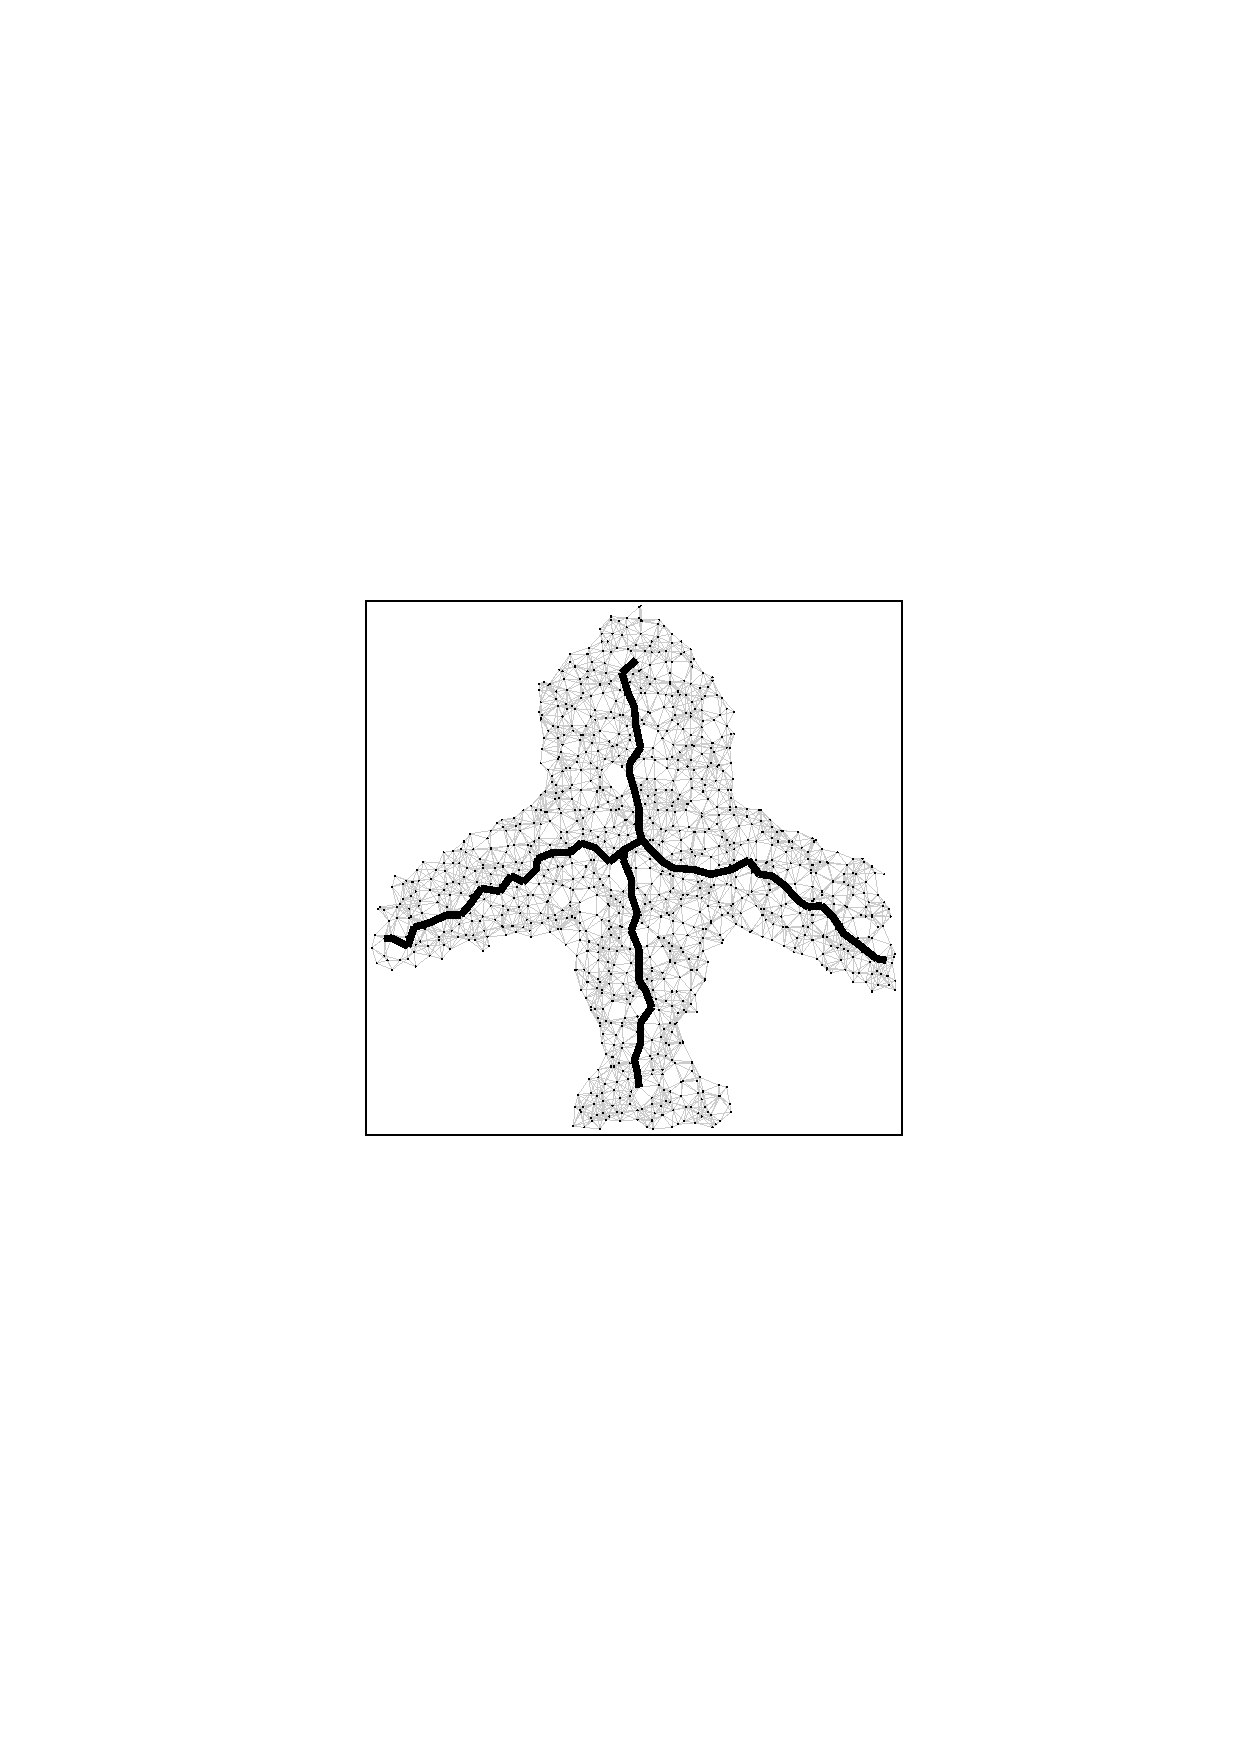
\includegraphics[width=.29\textwidth]{fig307-k}}\hspace{0.25em}%
  \subfloat[1524,10.92]{
    \label{fig:307l}
    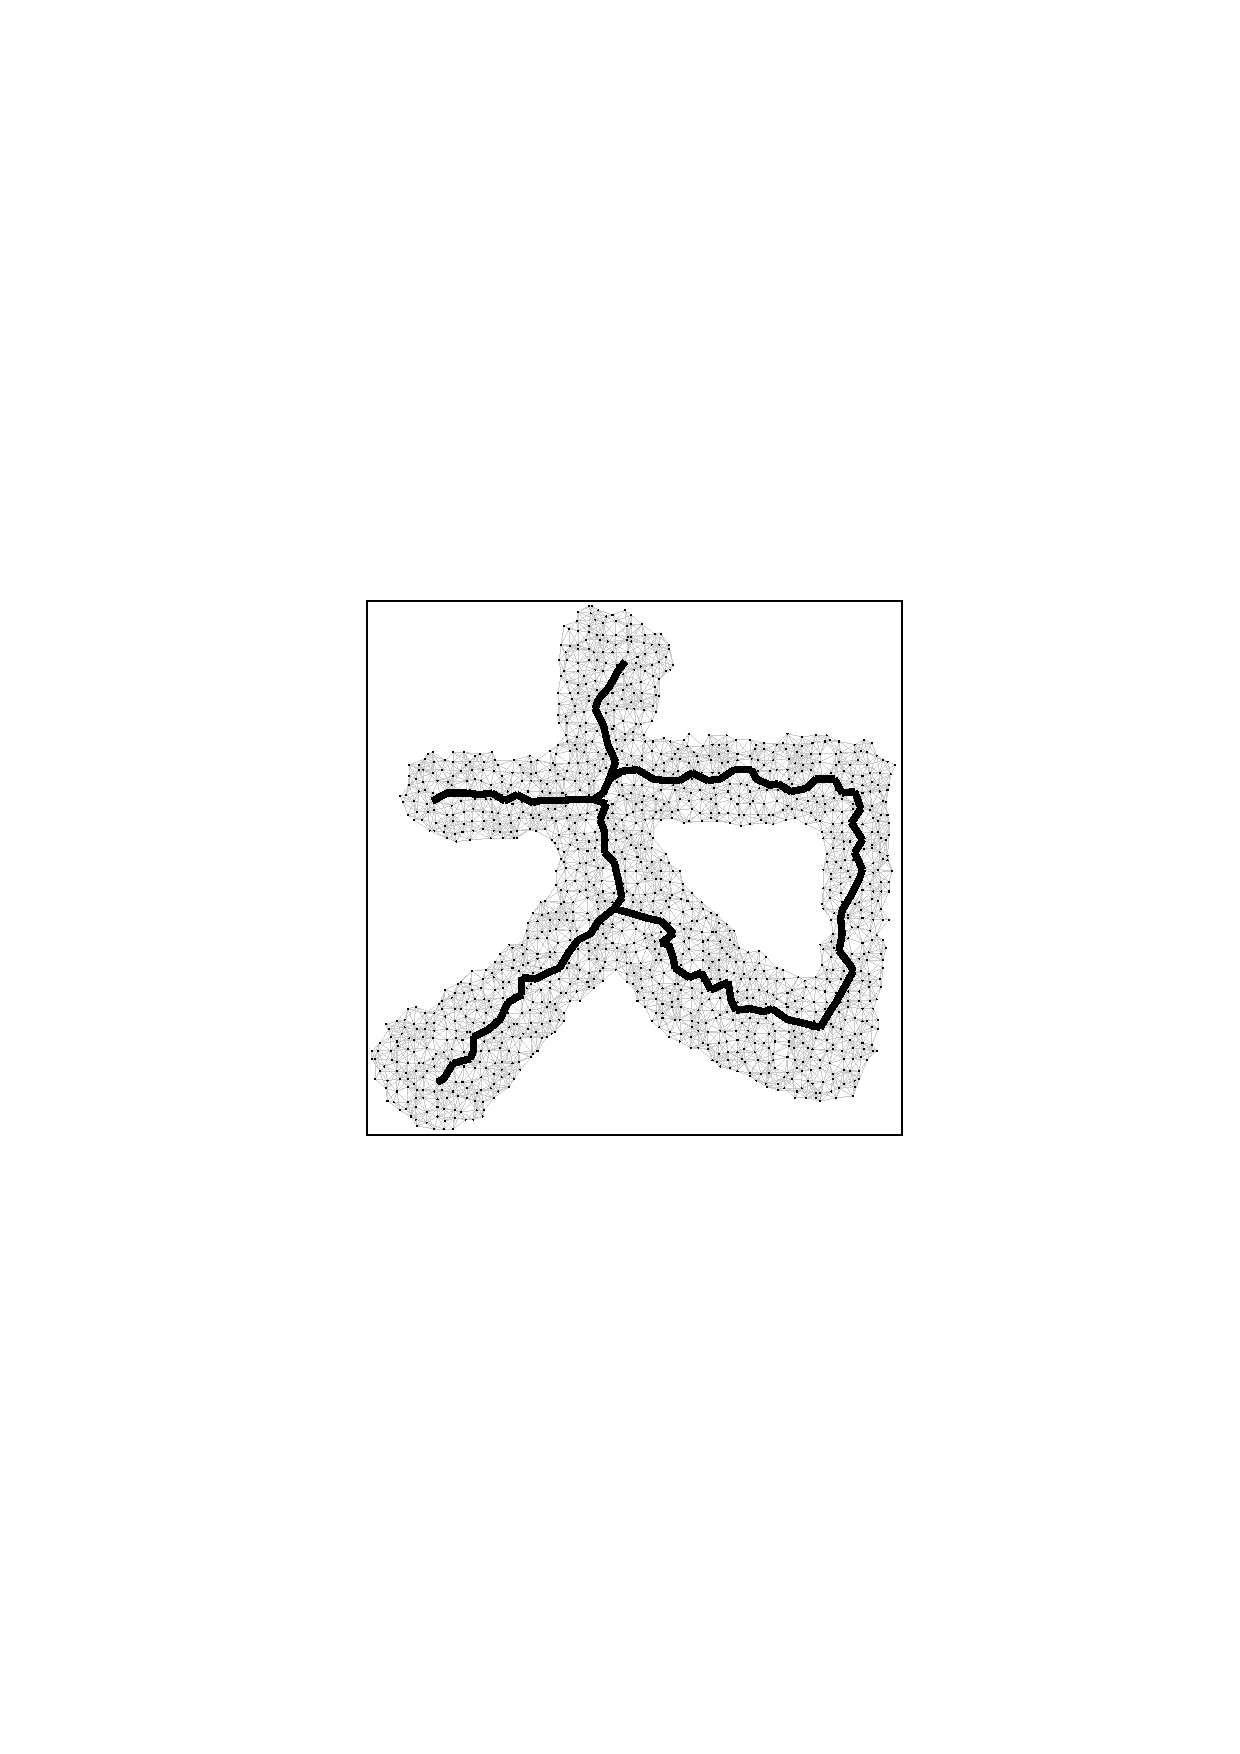
\includegraphics[width=.29\textwidth]{fig307-l}}
  \caption{拓扑骨干提取算法在不同形状的网络中的结果}
  \label{fig:307}
\end{figure}
\subsection{实验设置}
本章以及本文后续各章节中的仿真实验均是在MATLAB平台上进行。在仿真实验中,我们首先验证证拓扑骨干提取算法在具有多种不同形状的网络中的有效性,然后对一些可能影响到算法性能的参数进行分析,如节点部署模型和节点密度、通讯图模型等。节点部署模型采用随机部署和扰动网格两种方式。我们通过调整扰动网格的扰动系数来生成具有不同部署均匀性的网络。节点的平均密度通过调整通讯半径来调节,平均节点度的变化范围在5至20之间。通讯图模型分别采用UDG 和Q-UDG 模型。在边界识别组件中,我们统一地设置参数$k=3$,即每个节点对自身的3跳邻居子图执行MDS算法以判断是否为边界节点。而在骨干节点提取组件中,我们统一地设置参数$\delta=2$,即如果节点到边界的距离在2跳邻居范围内是局部最大化的则为骨干节点。在剪枝修正组件中,我们统一地设置参数$\lambda=\omega=10$,即原始骨干中长度小于10的环和分支将被删除。
\subsection{不同形状网络的实验结果}
\begin{figure}[t]
  \centering
  \subfloat[0.5-扰动网格]{
    \label{fig:308a}
    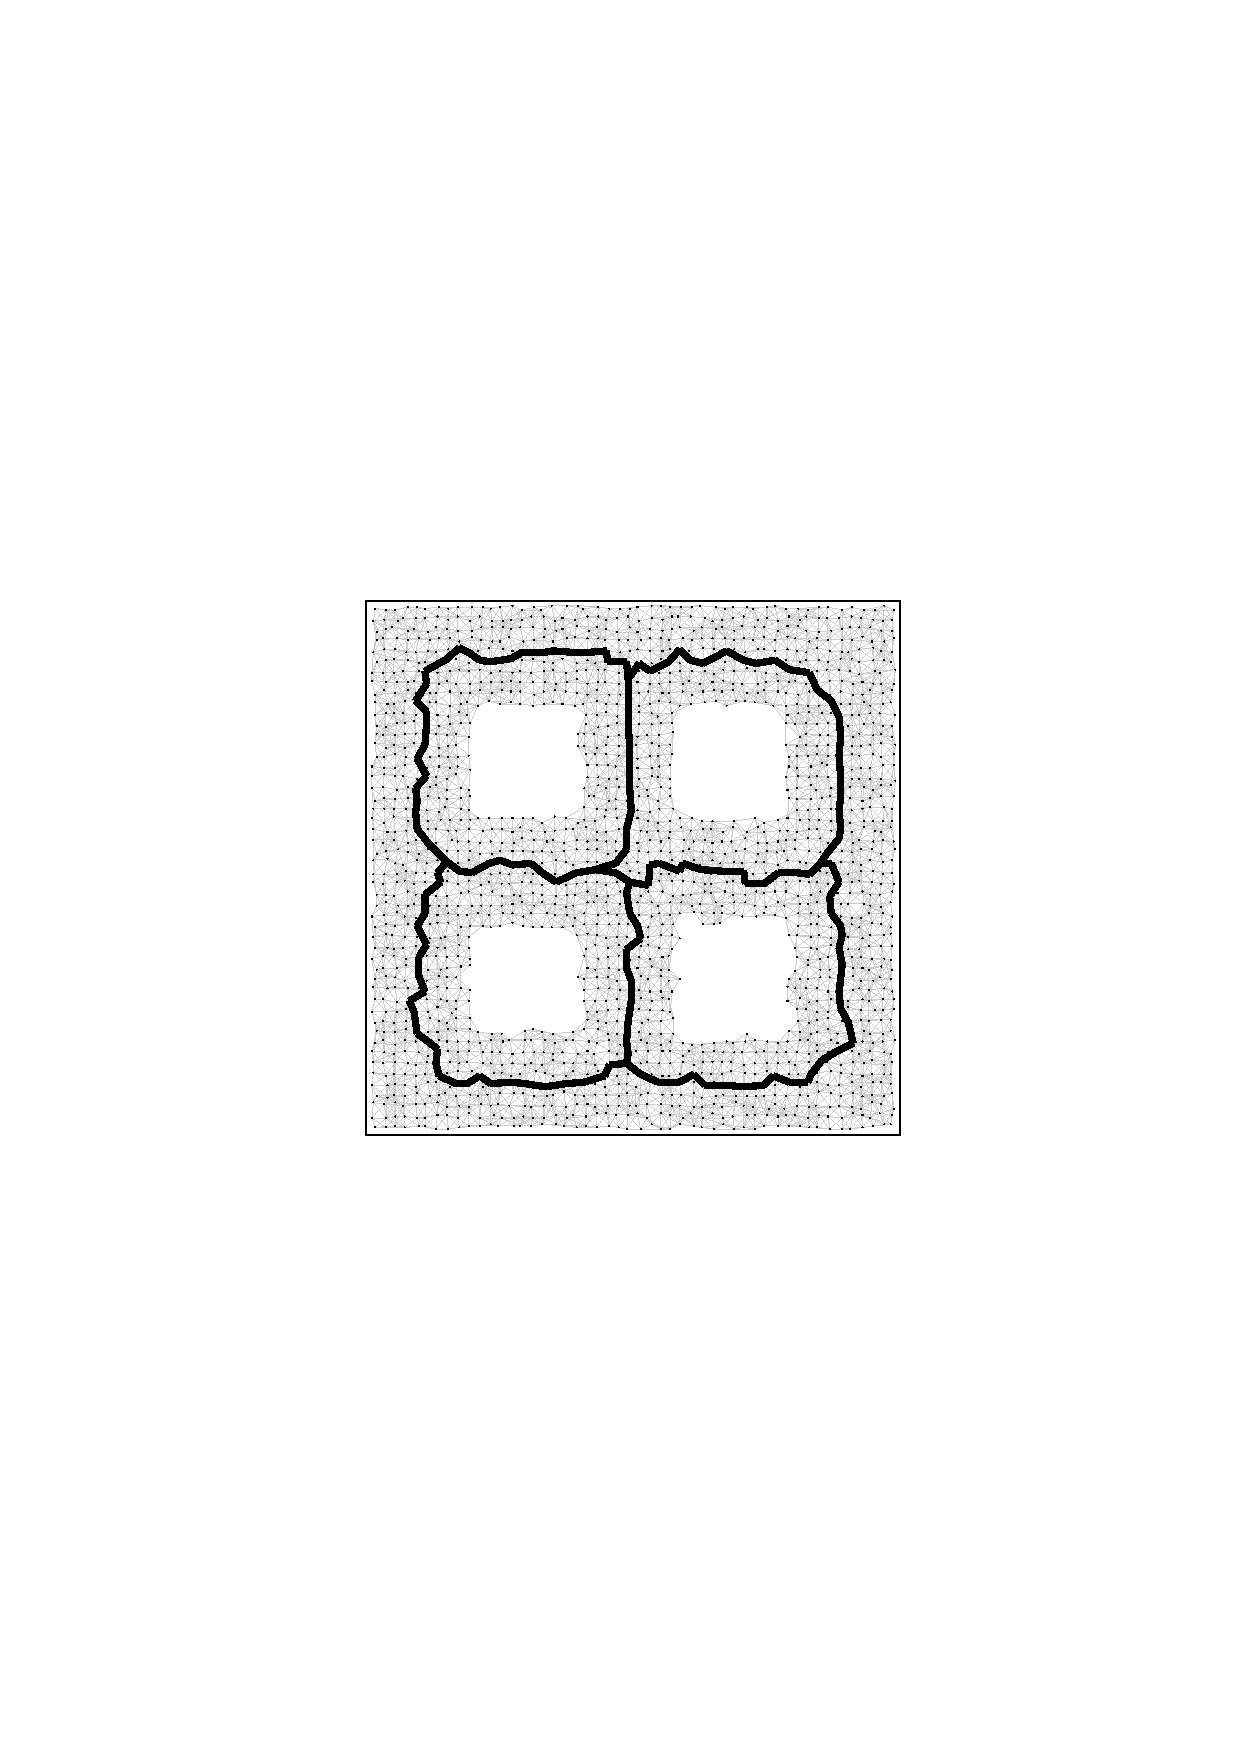
\includegraphics[width=.32\textwidth]{fig308-a}}\hspace{0.25em}%
  \subfloat[2-扰动网格]{
    \label{fig:308b}
    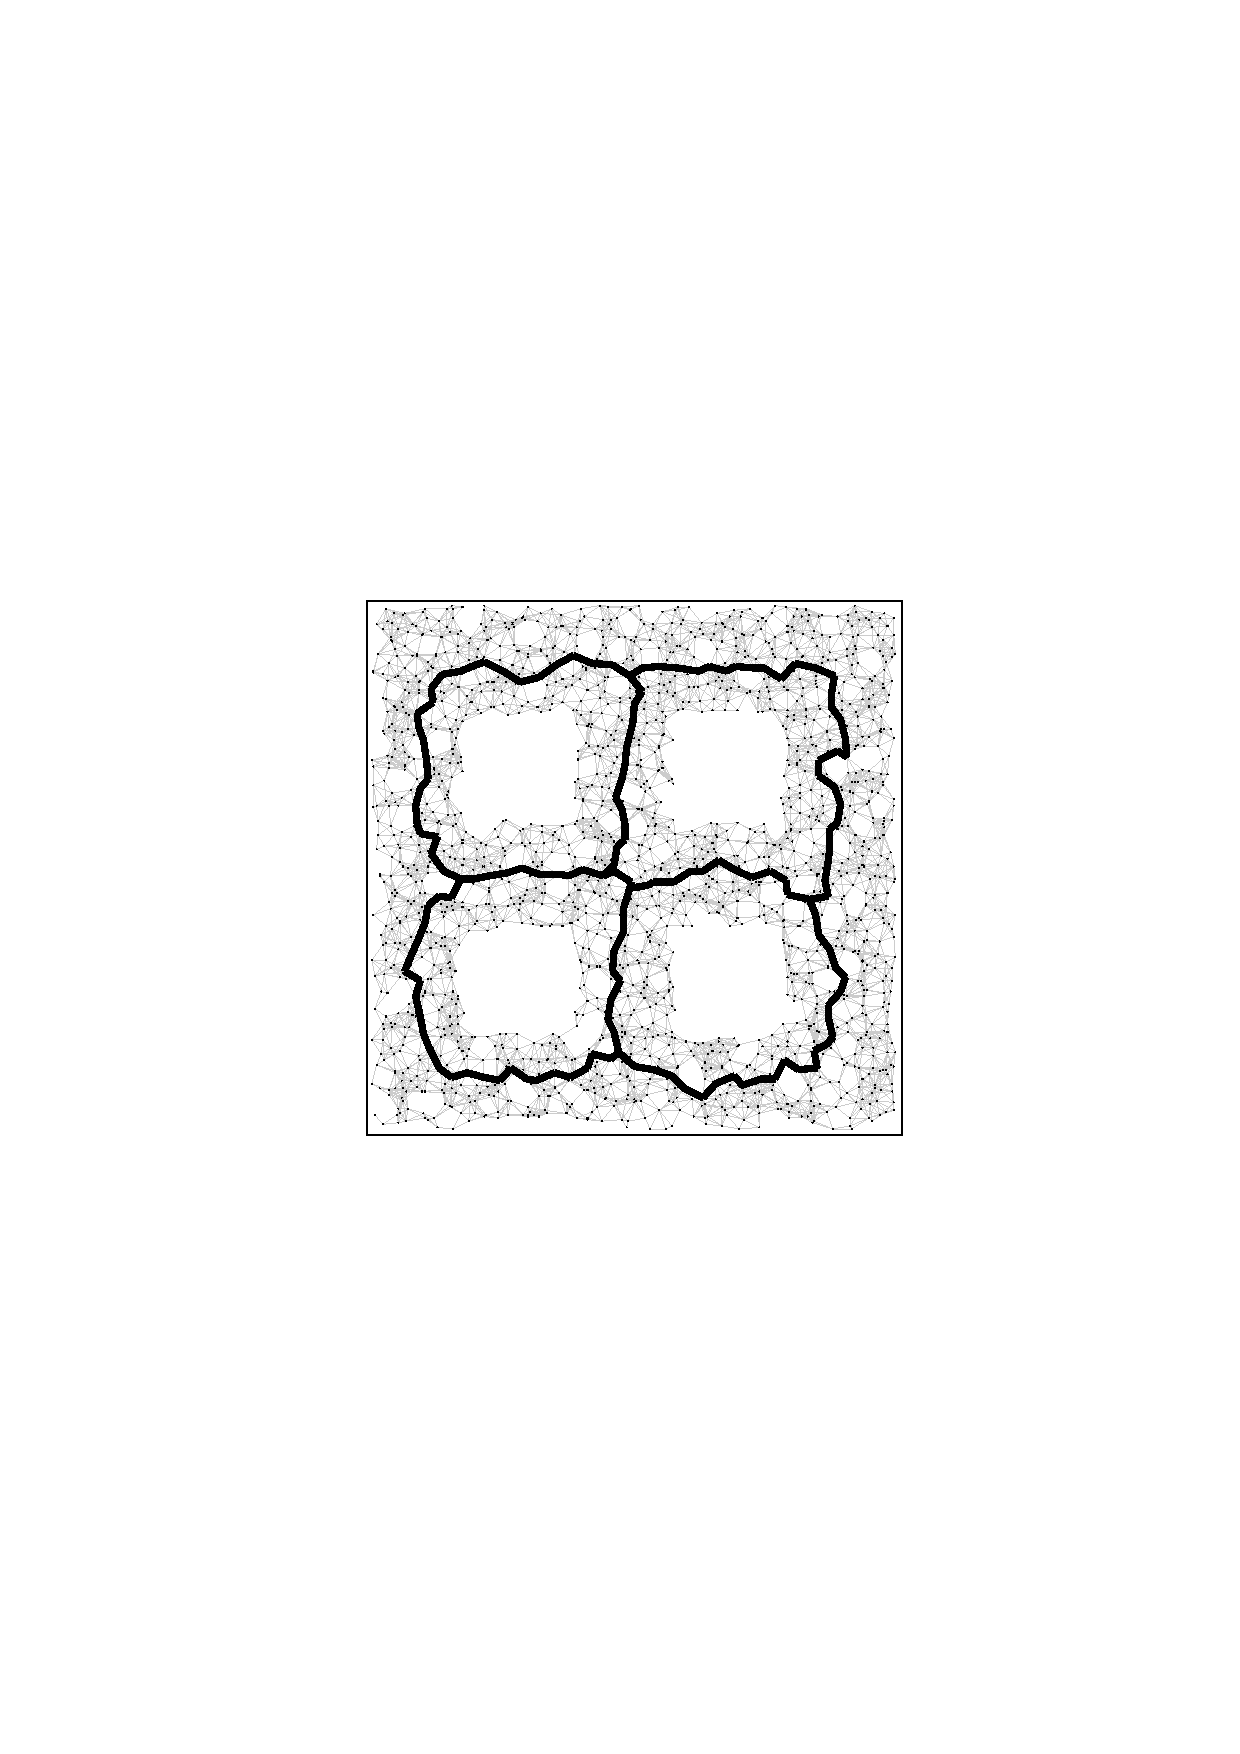
\includegraphics[width=.32\textwidth]{fig308-b}}\hspace{0.25em}%
  \subfloat[随机部署]{
    \label{fig:308c}
    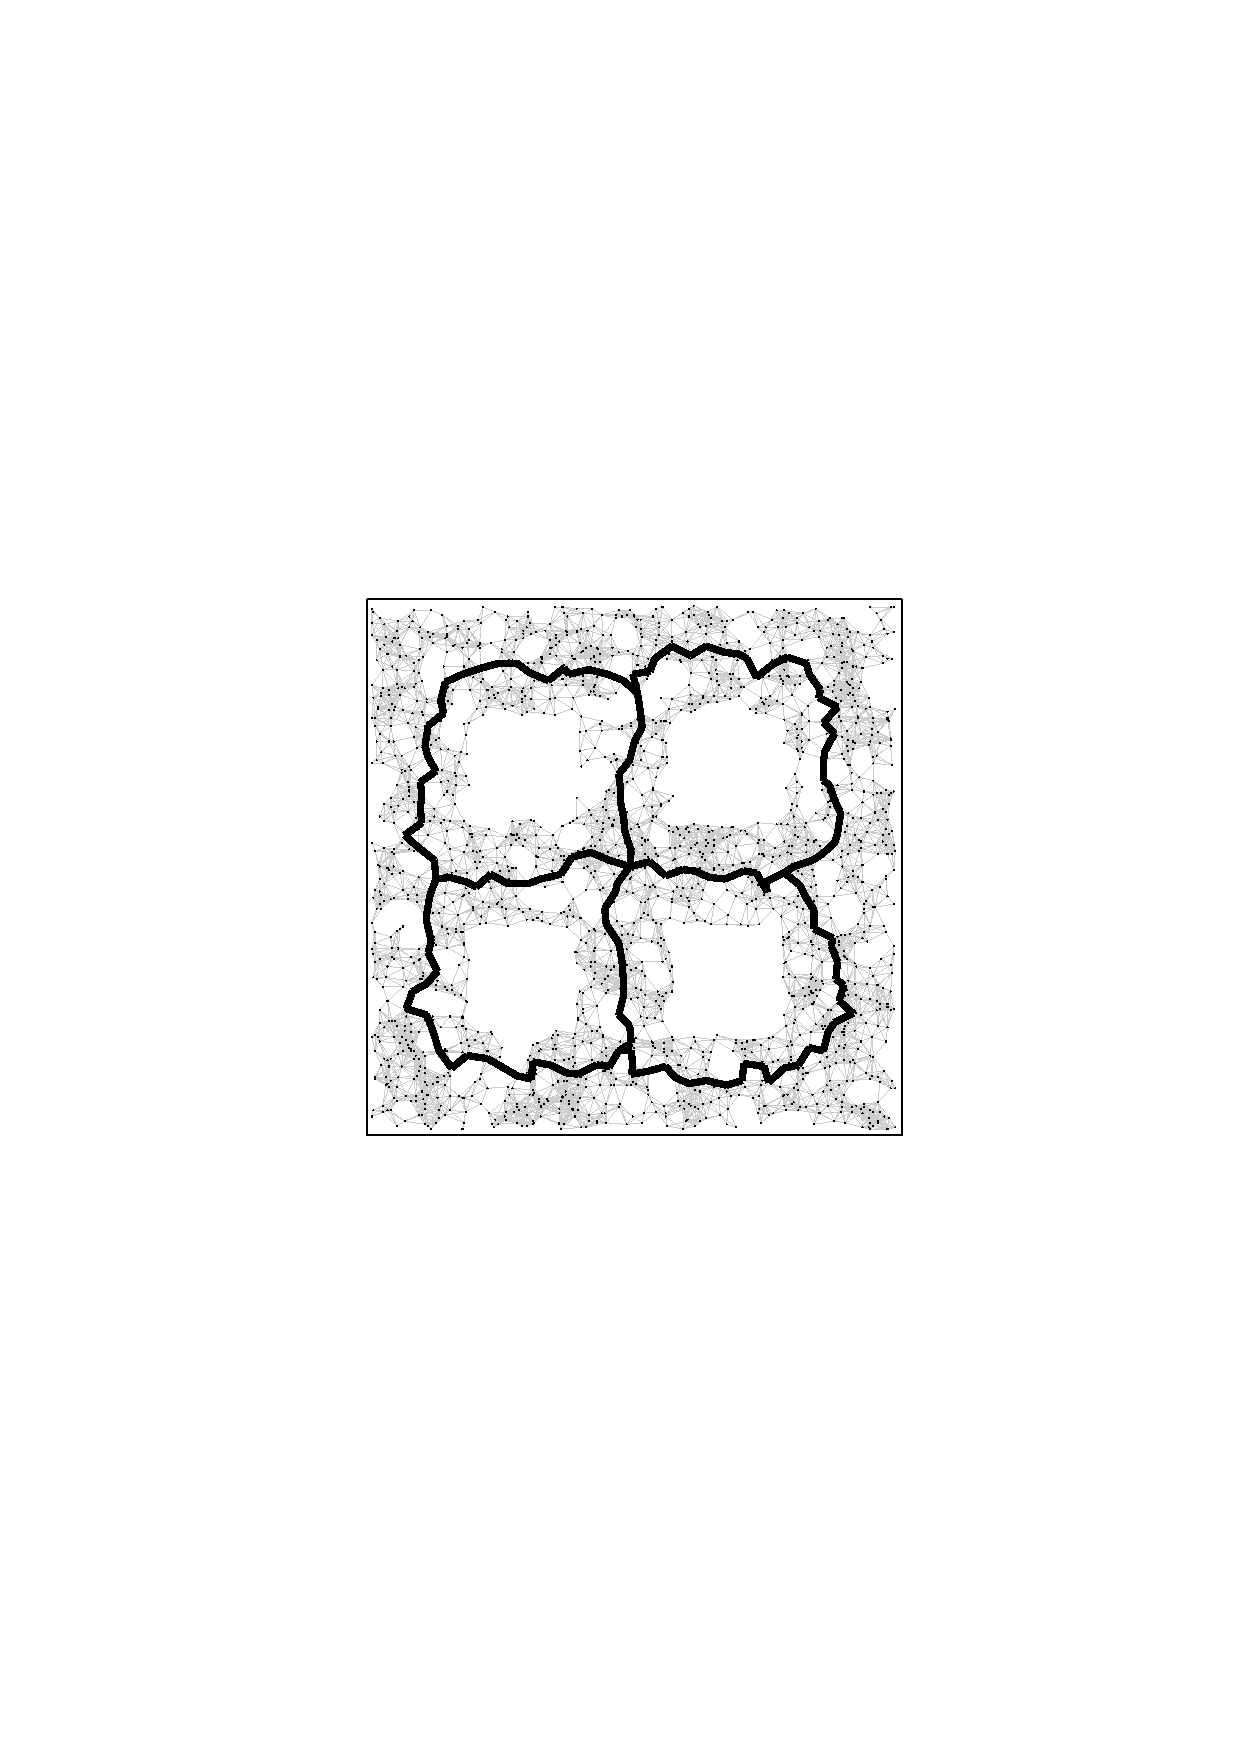
\includegraphics[width=.32\textwidth]{fig308-c}}
\caption{拓扑骨干提取算法在不同网络部署模型下的结果}
\label{fig:308}
\end{figure}
首先评估算法在不同形状网络中的有效性和性能,实验结果如图\ref{fig:307}所示。在本组实验中,所有的网络均采用0.75-Q-UDG模型以及扰动系数为1的扰动网格部署模型。每个子图下方的标题中给出了网络的基本参数,分别为节点数量和平均节点度。例如,在图\ref{fig:307a}所示的包含1572个节点,平均节点度为10.09的花朵形状的网络中,利用本章提出的拓扑骨干提取算法得到的骨干网络如图中粗线所示。可见,算法提取出的拓扑骨干具有良好的连通性,且非常符合实际网络的几何形状。对于图\ref{fig:307b}所示非常复杂的中国印形状的网络,算法的执行结果仍然非常的理想。另外,图\ref{fig:307c}-\ref{fig:307l}分别给出了算法在多种不同形状网络中的执行结果。我们在更多不同形状的网络中进行了实验,均获得了一致的实验结果,这里不再赘述。可见,本章提出的拓扑骨干提取算法能够有效地应用在各种不同形状的网络中,具有非常广泛的可用性和良好的性能。
\subsection{节点分布的影响}
接下来评估网络节点分布对算法性能的影响。
\begin{figure}[t]
  \centering
  \subfloat[平均节点度5.89]{
    \label{fig:309a}
    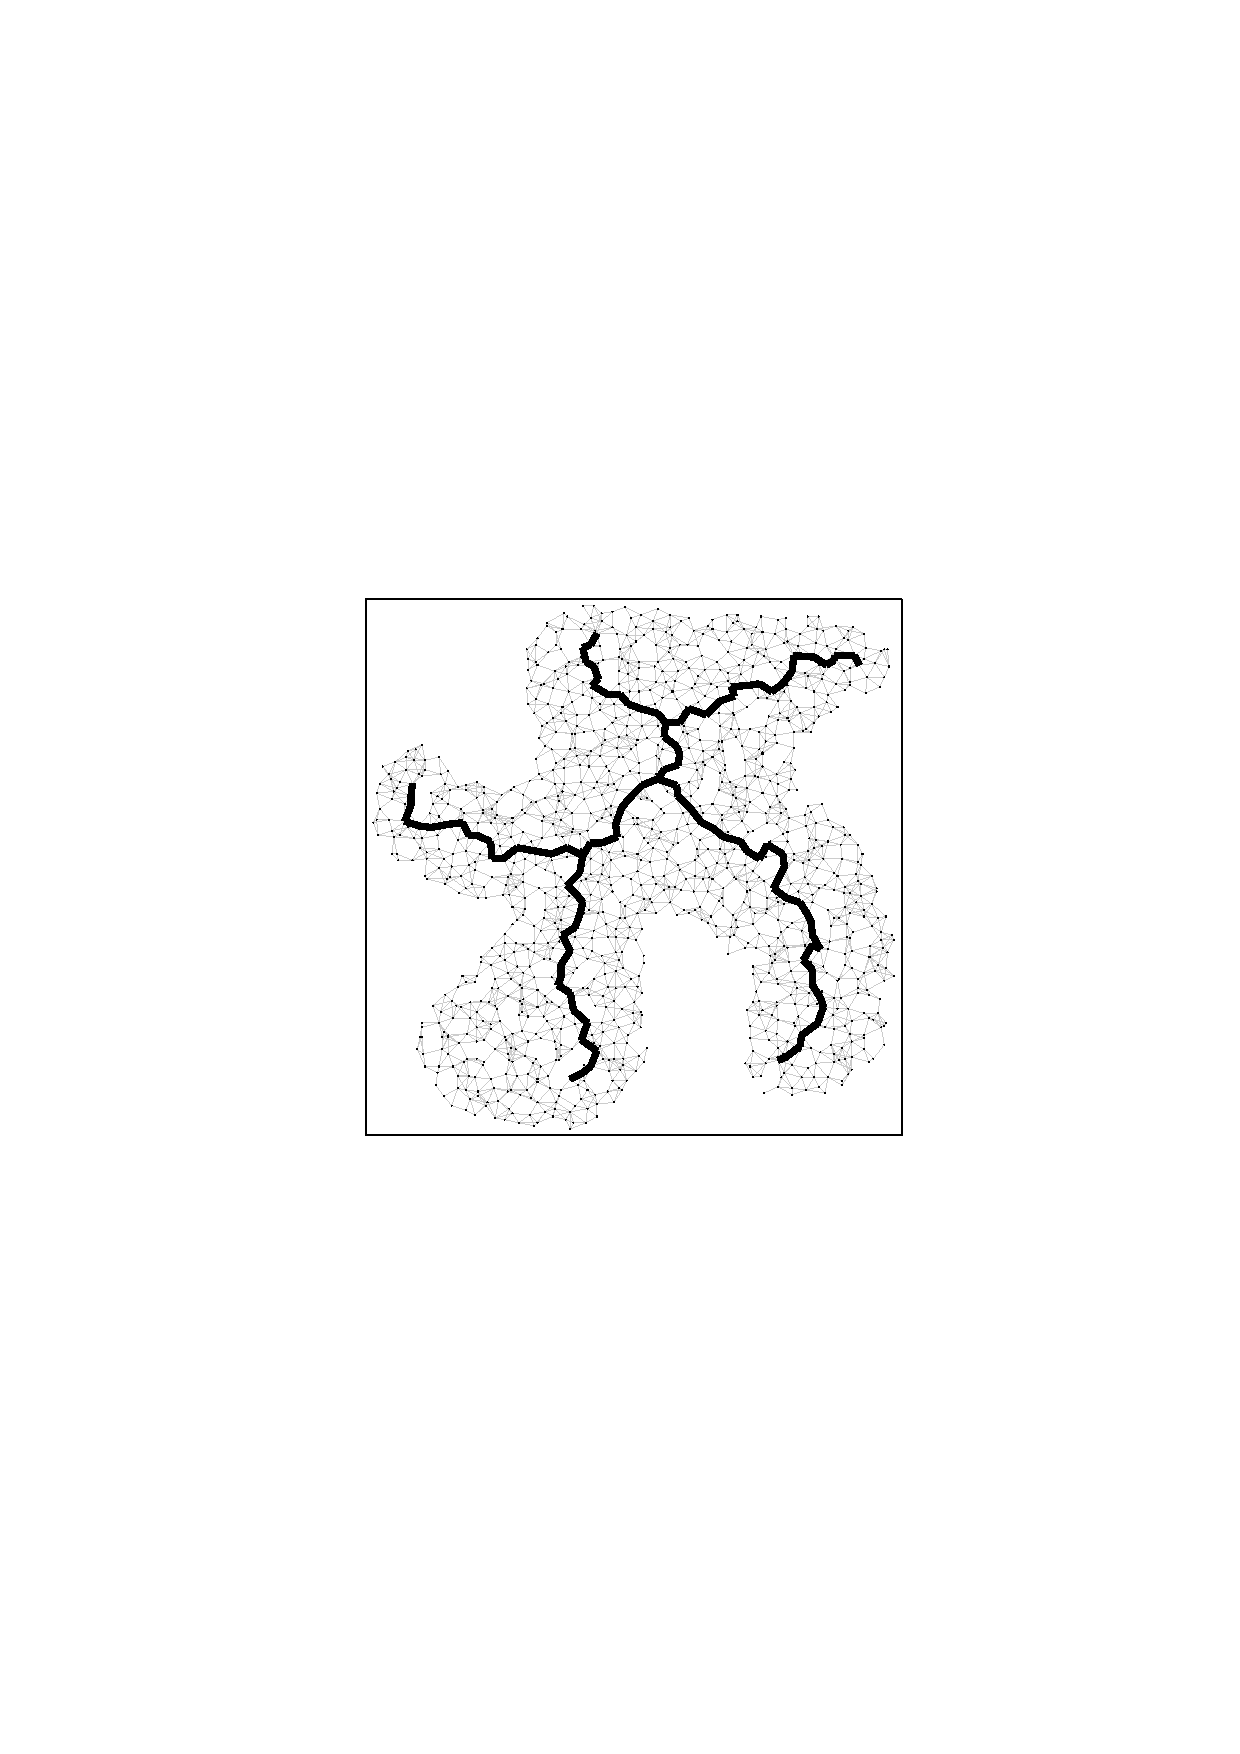
\includegraphics[width=.45\textwidth]{fig309-a}}\hspace{0.25em}%
  \subfloat[平均节点度15.96]{
    \label{fig:309b}
    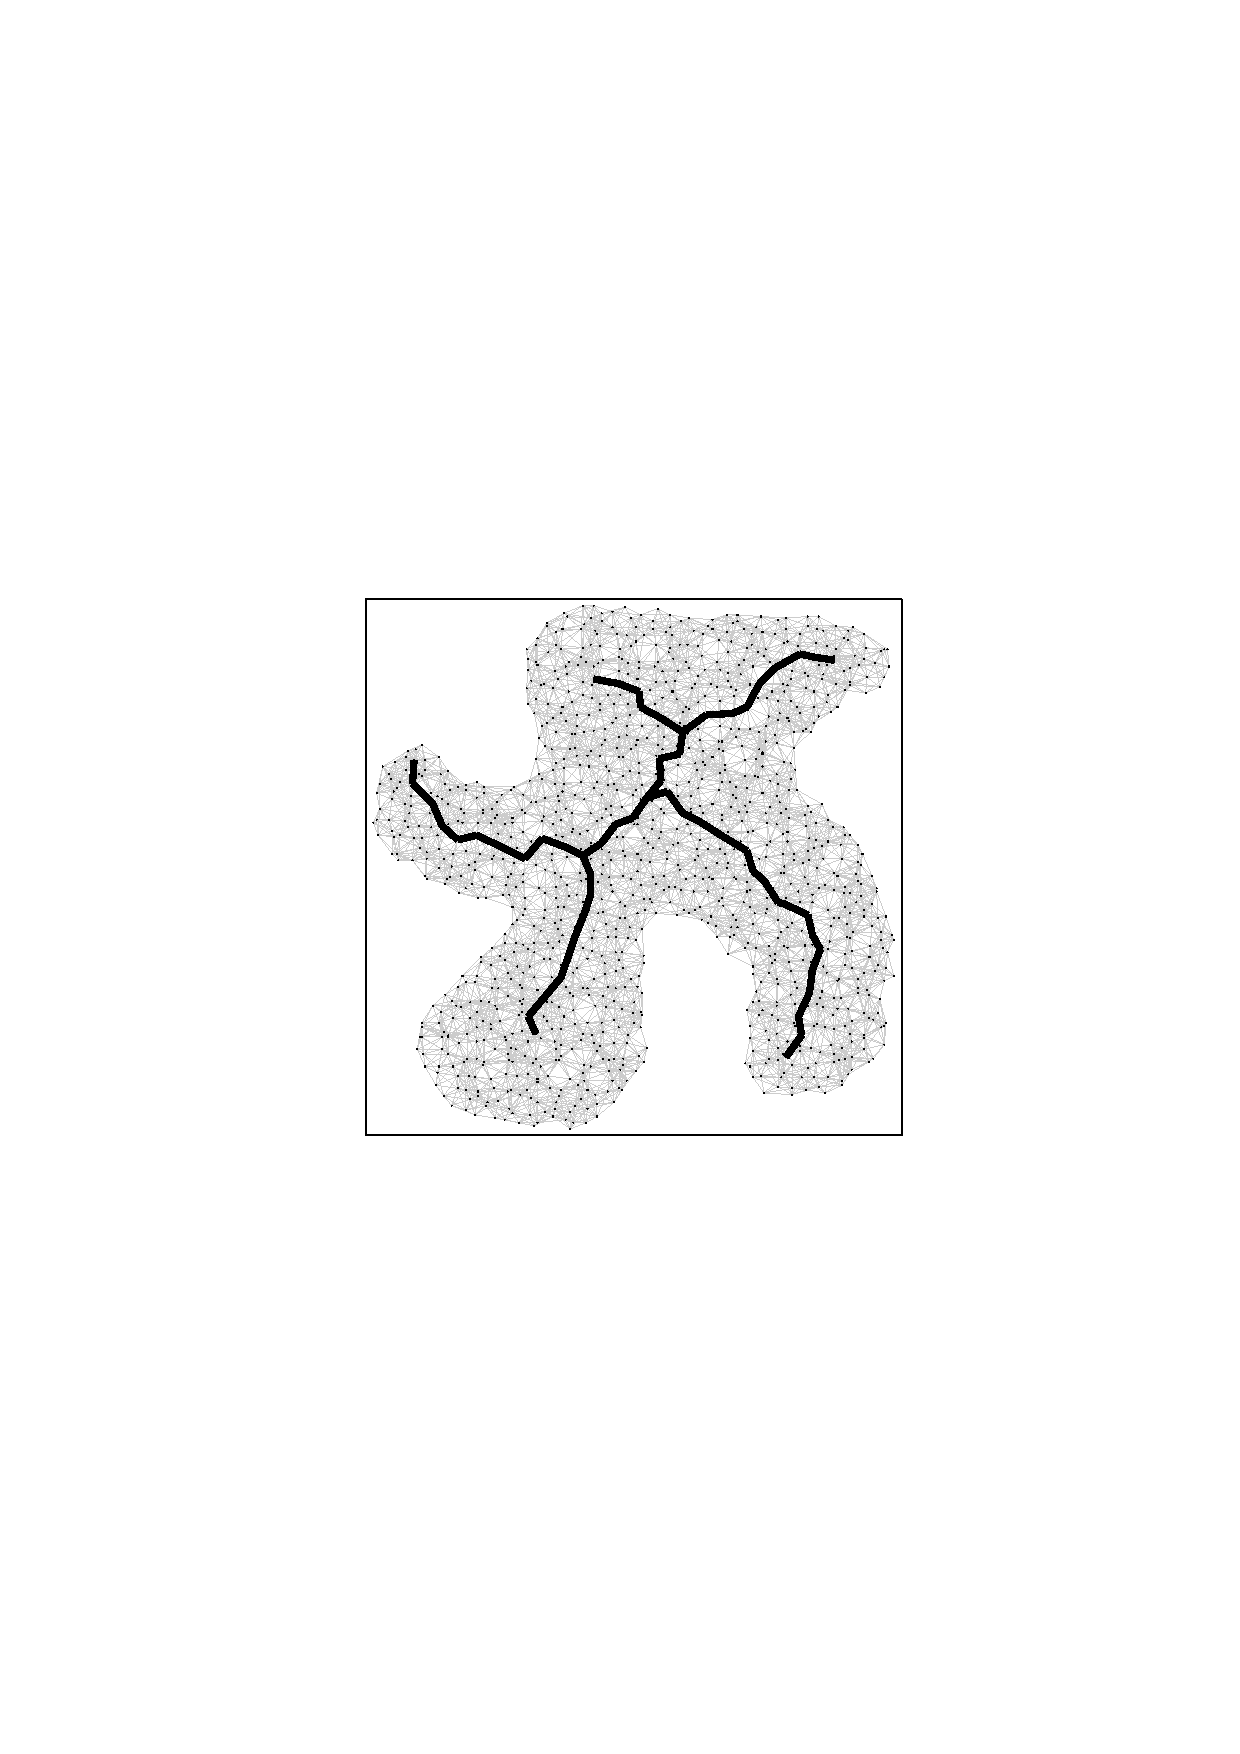
\includegraphics[width=.45\textwidth]{fig309-b}}\hspace{0.25em}%
  \subfloat[平均节点度5.93]{
    \label{fig:309c}
    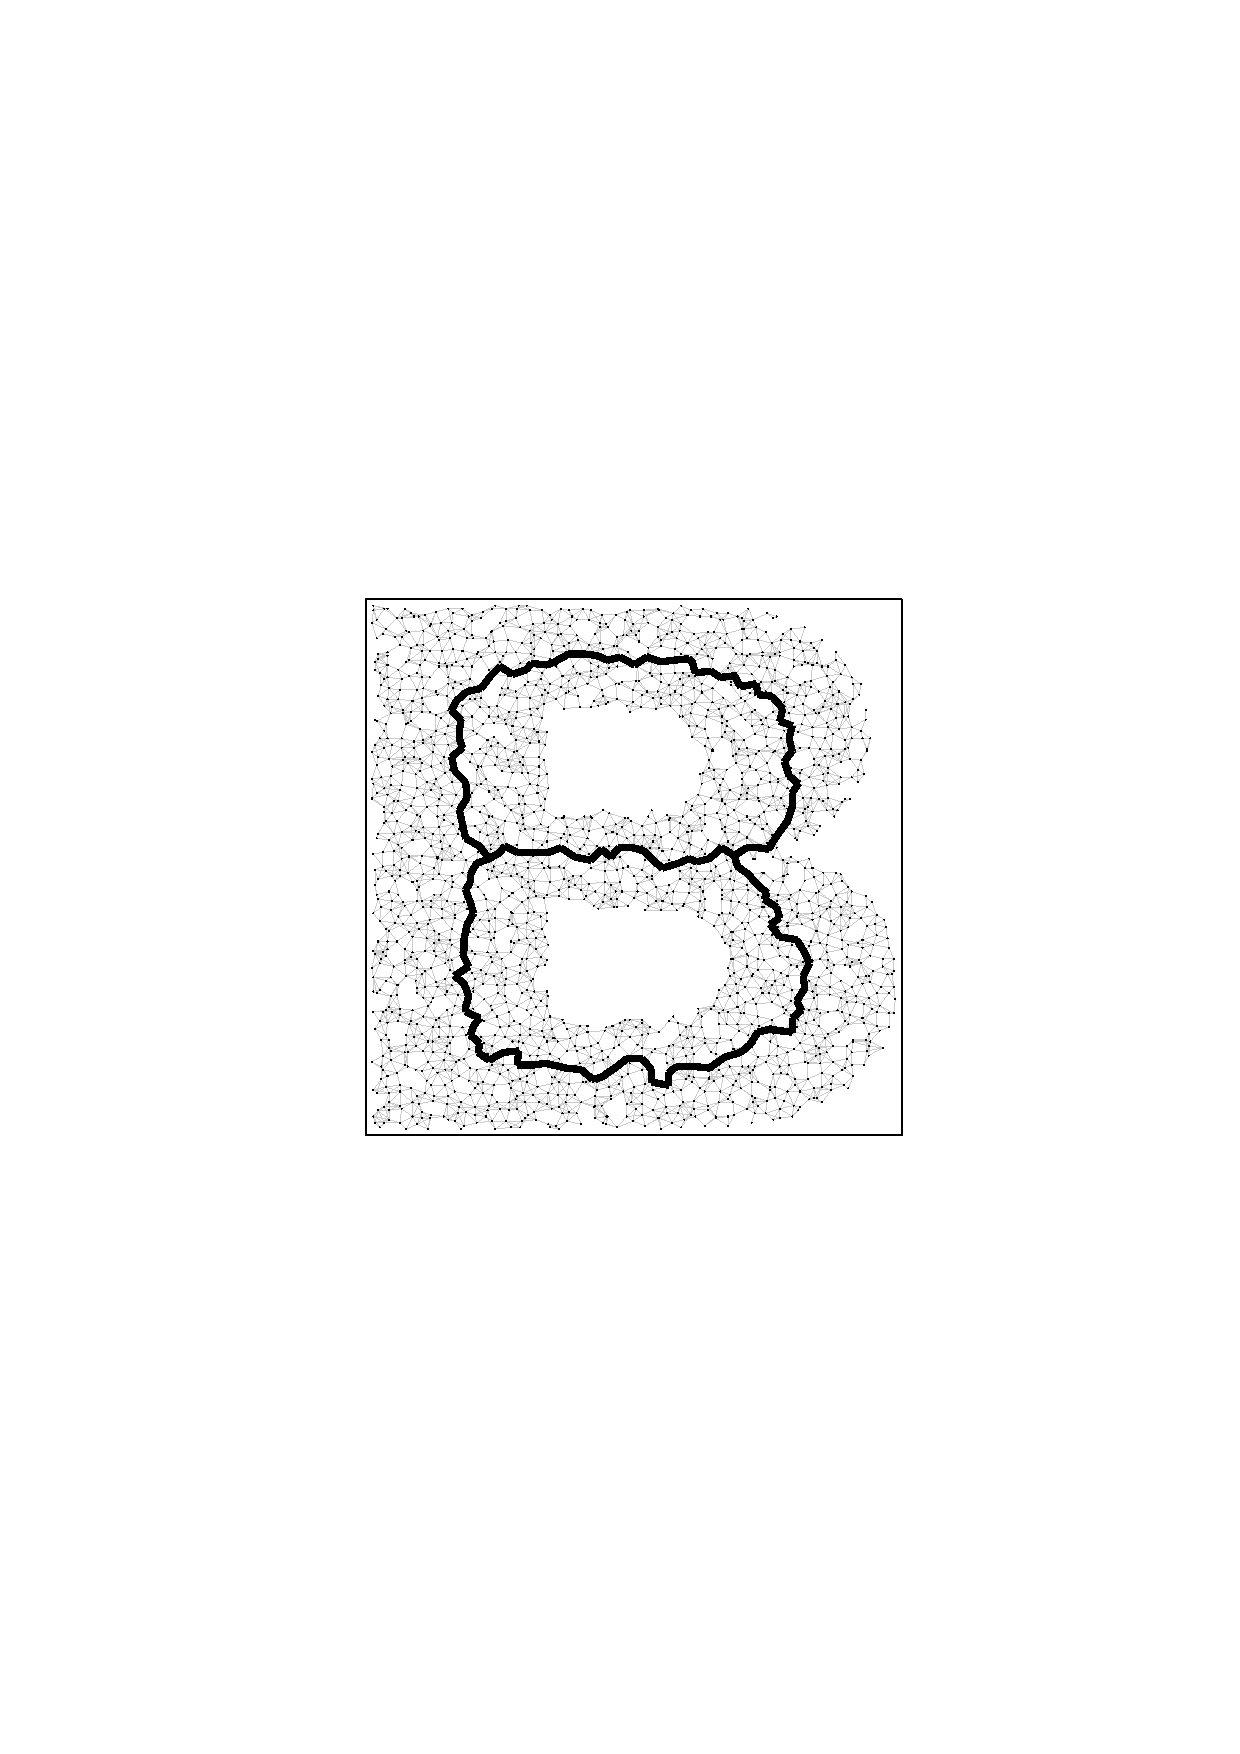
\includegraphics[width=.45\textwidth]{fig309-c}}\hspace{0.25em}%
  \subfloat[平均节点度15.67]{
    \label{fig:309d}
    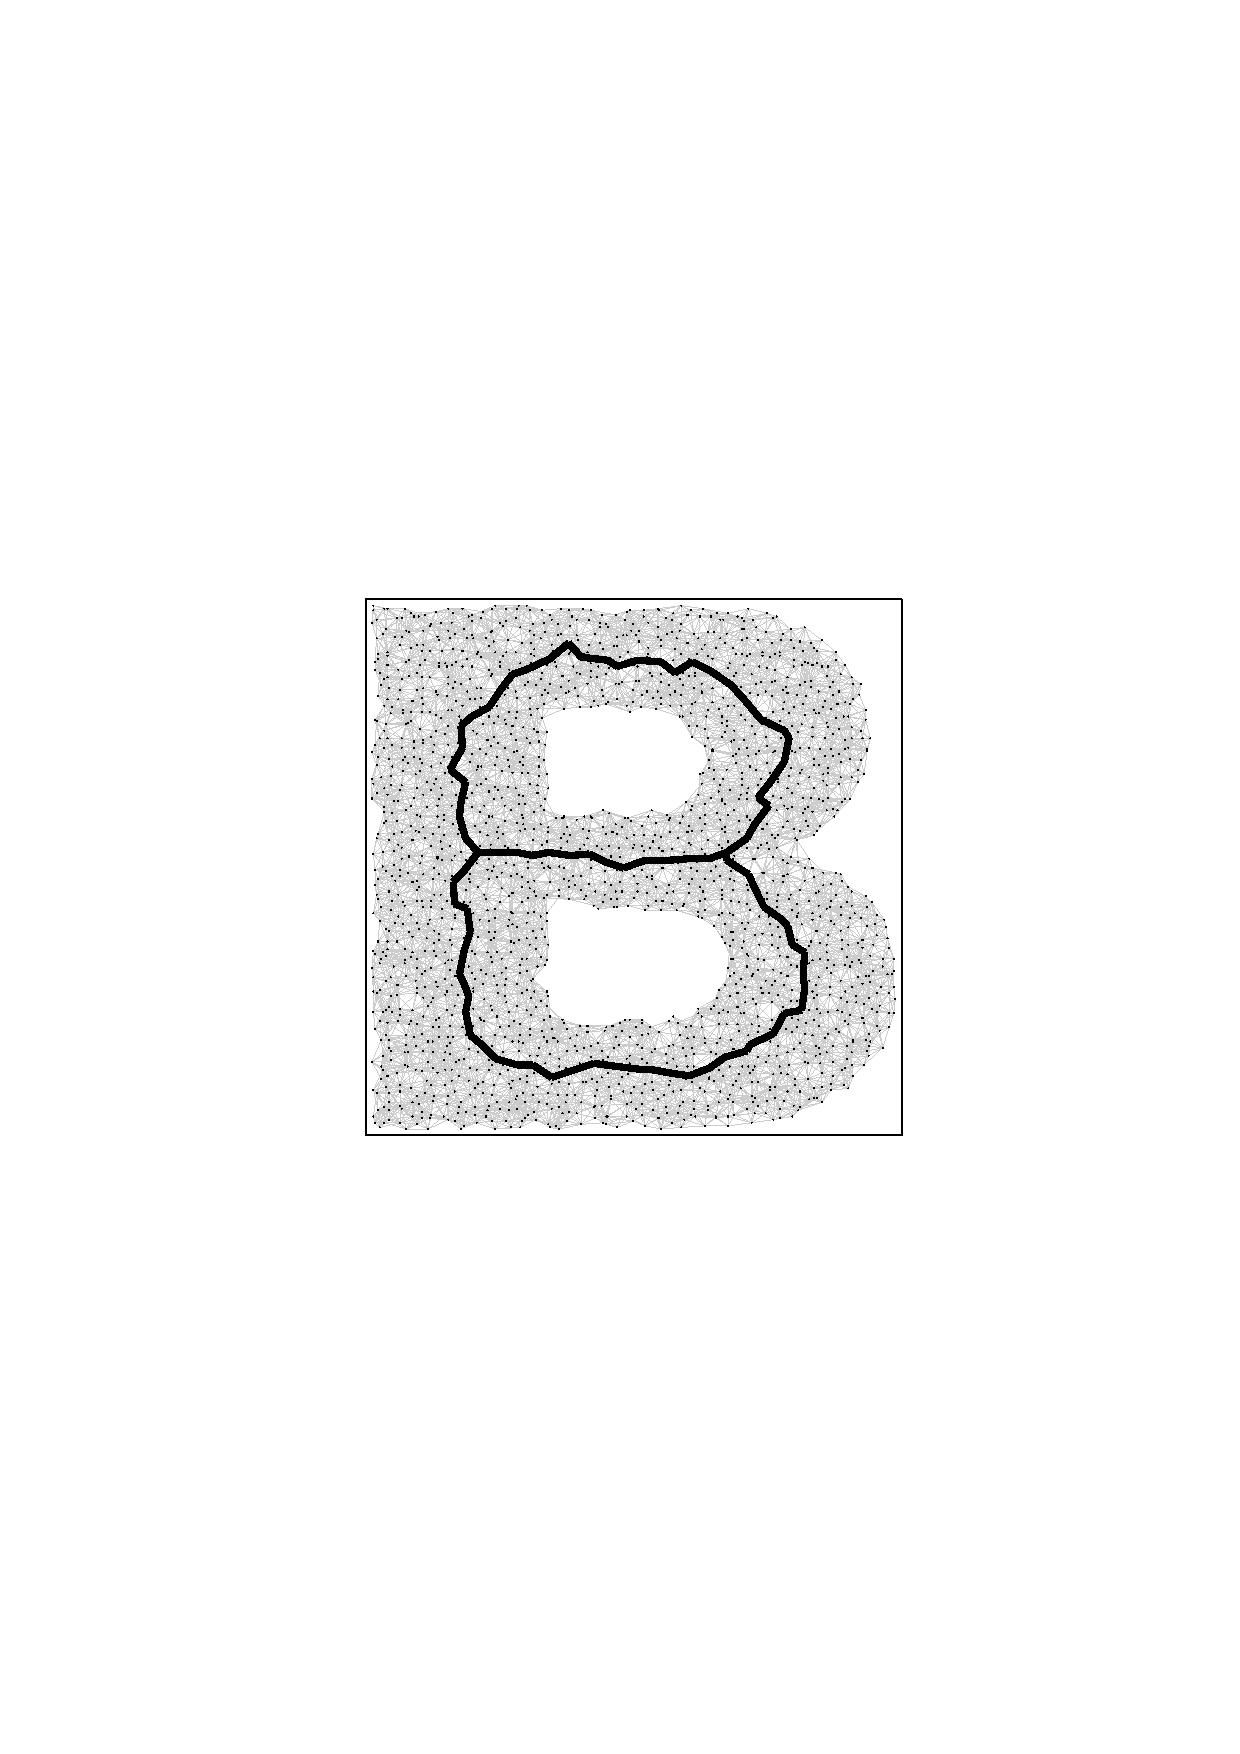
\includegraphics[width=.45\textwidth]{fig309-d}}
\caption{拓扑骨干提取算法在不同节点密度下的结果}
\label{fig:309}
\end{figure}

首先评估节点部署模型对算法性能的影响。我们分别采用了不同扰动系数的扰动网格模型和随机部署模型生成网络,并执行骨干提取算法,得到的结果如图\ref{fig:308}中所示。其中,图\ref{fig:308a}和图\ref{fig:308b}所示分别为扰动系数为0.5和2时的扰动网格模型下的结果,图\ref{fig:308c}所示为随机的节点部署模型下的结果。结合图\ref{fig:307e}中所示扰动系数为1的扰动网格模型下的结果可以看出,网络部署比较均匀时,算法得到的拓扑骨干更加平滑,随着网络部署随机性的增加,算法得到的拓扑骨干逐渐变得曲折。这是因为在随机性较强的网络中,节点及其之间的边的分布本来就是不平滑的,从而决定了无法获得平滑的拓扑骨干。需要强调的是,即使是在随机部署的网络中,算法得到的拓扑骨干始终具有较好的连通性,且能够很好地符合网络的实际形状。因此,算法对节点部署模型具有非常好的鲁棒性。

然后评估节点密度对算法性能的影响。我们验证算法在不同的平均节点度设置下的有效性和性能,实验结果如图\ref{fig:309}中所示。其中,图\ref{fig:309a}-\ref{fig:309b}分别给出了图\ref{fig:307c}中所示的网络(平均节点度为11.16)在平均节点度分别为5.89和15.96时的结果,而图\ref{fig:309c}-\ref{fig:309d}分别给出了图\ref{fig:307h}中所示的网络(平均节点度为11.14)在平均节点度分别为5.93和15.67时的结果。可见,算法在节点密度较高时得到的拓扑骨干更加平滑,节点密度较低时得到的拓扑骨干逐渐变得曲折。这是由于网络变得稀疏时,网络中边本身的分布也变得不再平滑。但在稀疏网络中,拓扑骨干仍然具有良好的连通性,并很好地反映了网络实际的形状。因此,算法对节点密度也具有很好的鲁棒性。
\subsection{通讯图模型的影响}
下面评估网络通讯图模型对算法性能的影响,比较算法在UDG和Q-UDG模型下的有效性和性能。
\begin{figure}[h]
  \centering
  \subfloat[]{
    \label{fig:310a}
    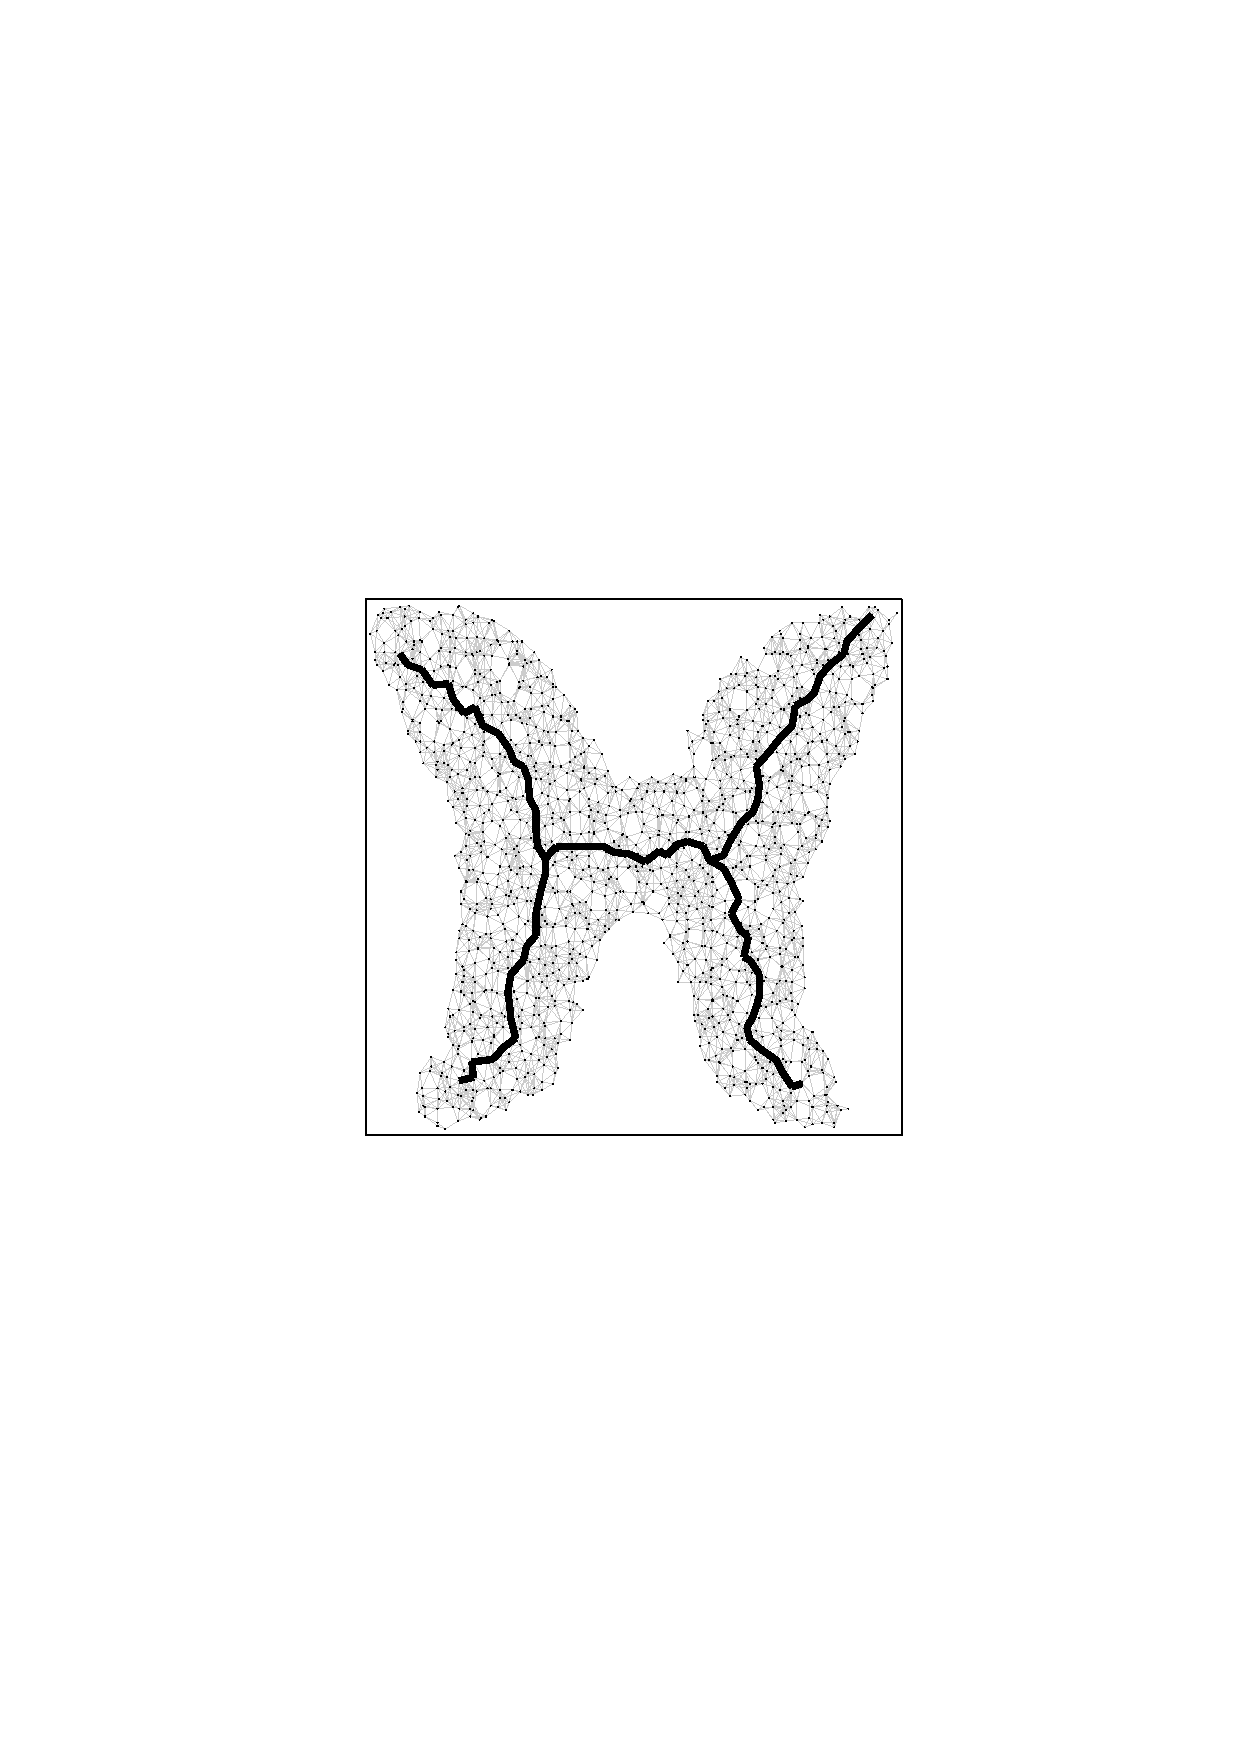
\includegraphics[width=.32\textwidth]{fig310-a}}\hspace{0.25em}%
  \subfloat[]{
    \label{fig:310b}
    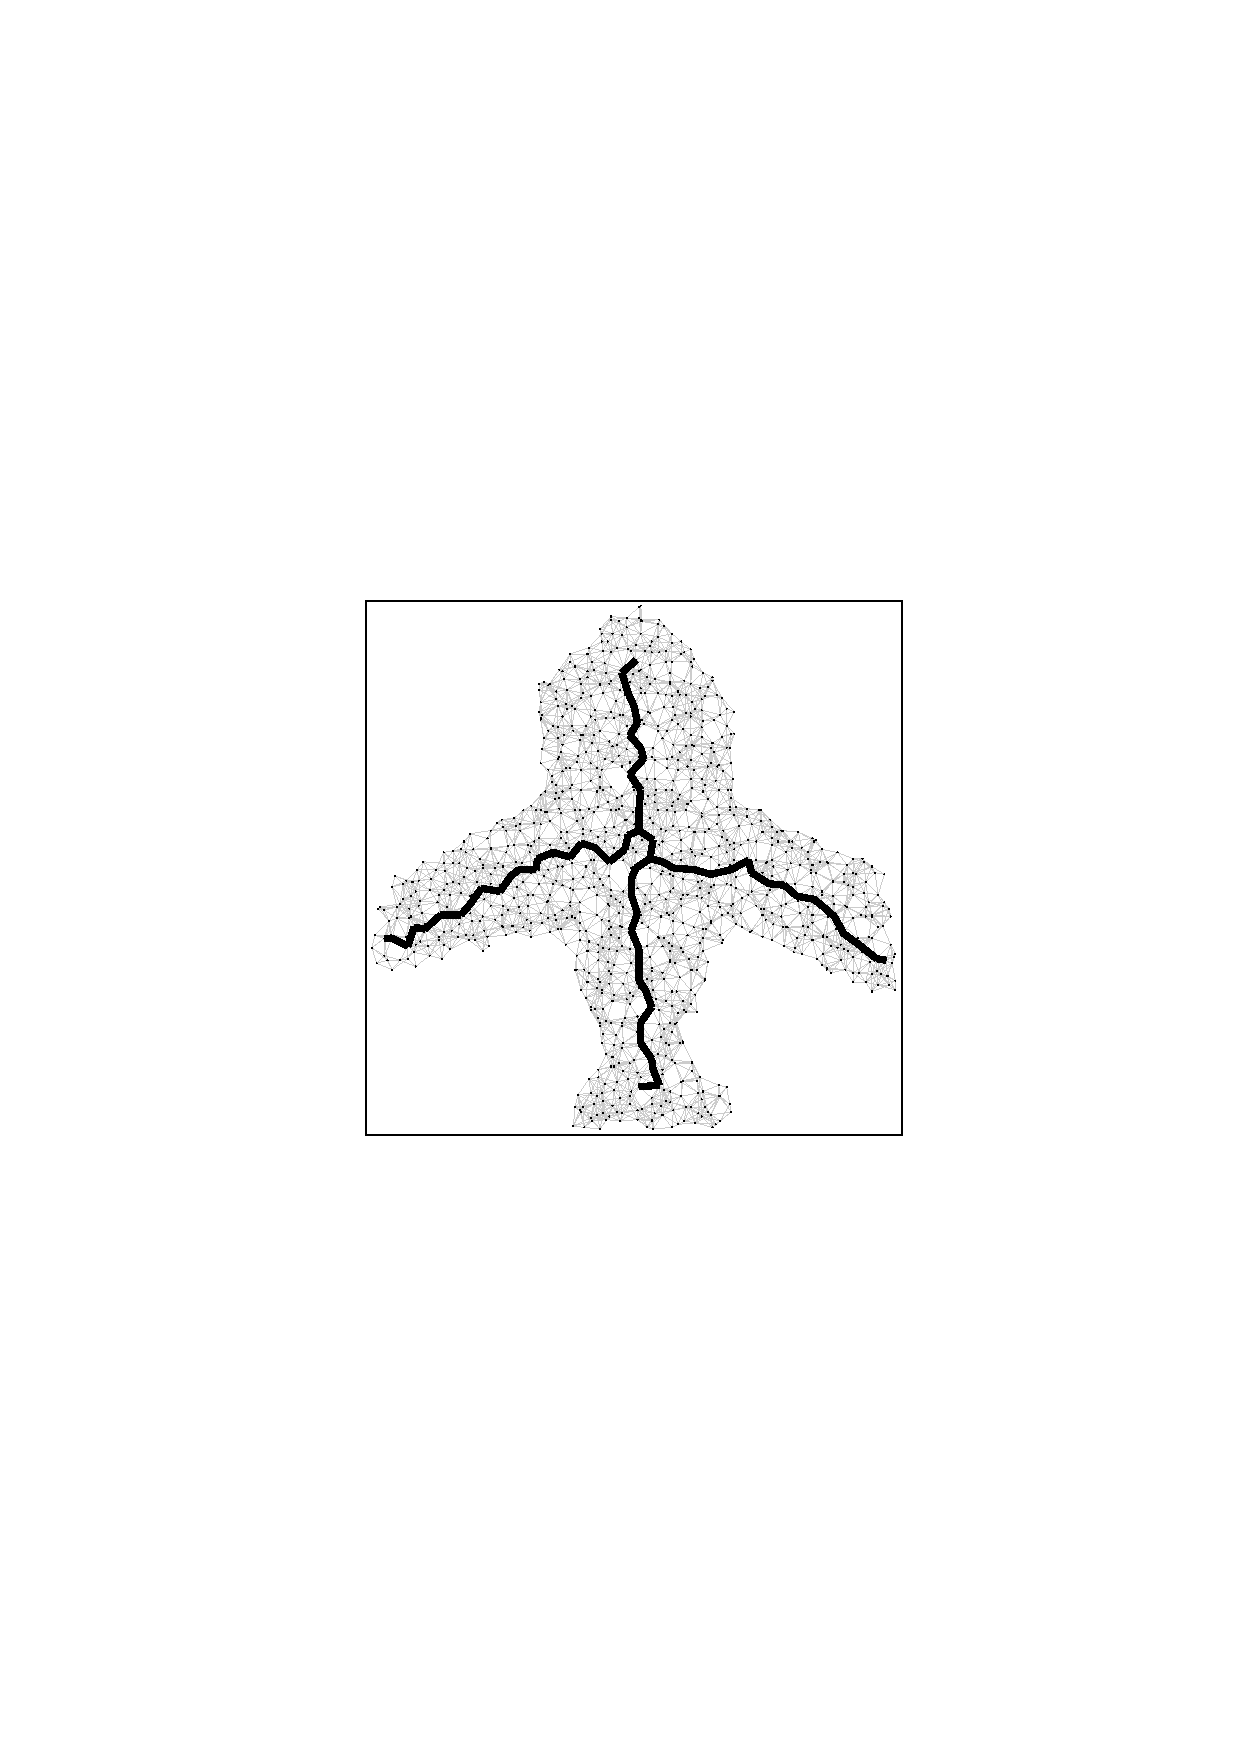
\includegraphics[width=.32\textwidth]{fig310-b}}\hspace{0.25em}%
  \subfloat[]{
    \label{fig:310c}
    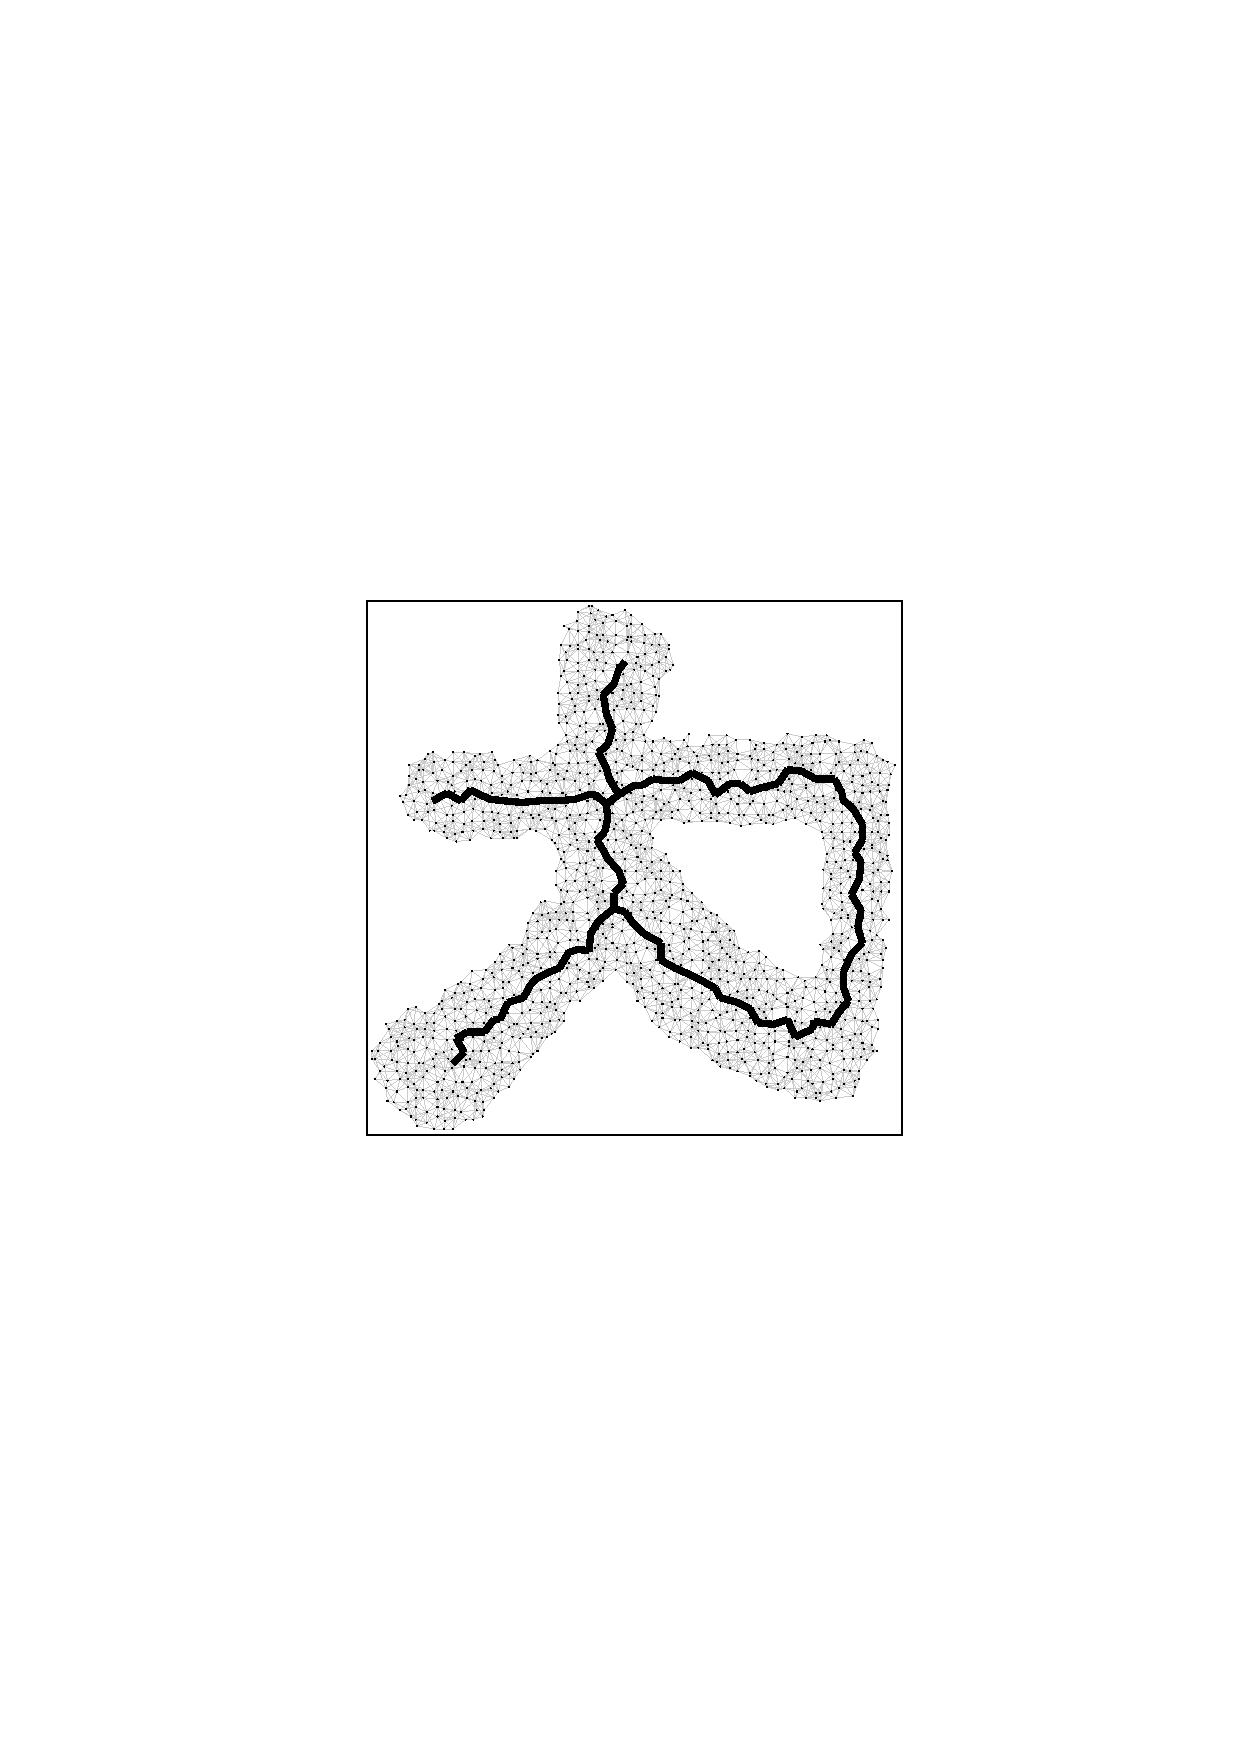
\includegraphics[width=.32\textwidth]{fig310-c}}
\caption{拓扑骨干提取算法在UDG模型下的结果}
\label{fig:310}
\end{figure}

图\ref{fig:307}所示均为算法在0.75-Q-UDG模型下的结果,而图\ref{fig:310}给出了算法在UDG模型下的结果。其中,图\ref{fig:310a}-\ref{fig:310c}分别给出了图\ref{fig:307j}-\ref{fig:307l}中所示的网络在对应的UDG模型下的结果。可见,采用不同的通讯图模型对算法的性能并没有明显的影响,从而验证了算法对通讯图模型的鲁棒性。从本质上来讲,在节点部署情况和节点通讯半径均相同时,采用UDG或Q-UDG模型只是改变了节点之间边的生成情况。具体来讲,UDG模型比Q-UDG 模型生成更多的边,因此产生更高的平均节点度(但差别并不显著)。由于算法对节点密度具有很好的鲁棒性,因此其性能也不受通讯图模型的影响。
\section{本章小结}
本章研究了无线传感器网络中不依赖位置信息的拓扑骨干提取问题。目前已有的不依赖位置的拓扑骨干提取算法大部分依赖特殊的网络假设,缺乏在稀疏或随机部署网络条件下的鲁棒性,或无法提取出确定性的、符合实际的网络形状的拓扑骨干。本章针对已有方法的局限性,提出了一种仅依赖局部连通性信息,具有良好鲁棒性的拓扑骨干提取算法。算法设计和利用了仅依赖局部连通性信息的基于MDS的边界识别算法及一种高效的图变换工具HPT,并巧妙地设计了一种骨干叶节点的判定方法。本章通过理论证明以及大量的仿真实验验证了所提出算法的有效性和性能。实验结果显示,算法能够有效地适用于具有各种不同复杂形状和参数设置的网络,提取出高质量的拓扑骨干。
